%!TEX root = root.tex

\chapter{Robust Generalizations of the Law of Large Graphs}
\label{chap:robust_llg}

While Chapter~\ref{chap:llg} makes an effort to estimate the mean of a collection of unweighted graphs, we shift our focus to weighted graphs under a more general setting in this chapter.
In the general parametric framework, $G \sim f \in \mathcal{F} = \{f_{\theta} : \theta \in \Theta \}$, and selecting a principled and productive estimator $\hat{\theta}$ for the unknown graph parameter $\theta$ given a sample of graphs $\{G^{(1)}, \cdots, G^{(m)}\}$ is one of the most foundational and essential tasks, facilitating subsequent inference.
For example, \citet{ginestet2014hypothesis} proposes a method to test for a difference between the networks of two groups of subjects in functional neuroimaging; while hypothesis testing is the ultimate goal, estimation is a key intermediate step.
Note that this setting is more general since in Chapter~\ref{chap:llg}, estimating the mean of a collection of unweighted graphs is equivalent to estimating $\theta$ when $\mathcal{F}$ are Bernoulli distributions.
We propose a widely-applicable, robust, low-rank estimation procedure for a collection of weighted graphs.

Consider for illustration the connectome data set made available through the
Consortium for Reliability and Reproducibility\footnote{\url{http://fcon_1000.projects.nitrc.org/indi/CoRR/html/}}
and investigated in Section~\ref{sec:robust_LLG_corr_data} below.
We have $m=114$ brain graphs, each having $n=70$ vertices representing different anatomical regions; the (errorfully observed) weight of an edge between two vertices represents the number of white-matter tracts connecting the corresponding two regions of the brain, as measured by diffusion tensor magnetic resonance imaging.
Our goal in this situation is to estimate the average number of white-matter tracts between different regions of the brain. A more accurate estimate can lead to a better understanding of brain connectivity and hence functionality. Also, better estimates will improve performance on other tasks, such as diagnosis of brain disease.

The maximum likelihood estimate (MLE) -- the edge-wise sample mean, without taking any graph structure into account, as in the (weighted extension of) the independent edge graph model (IEM) \citep{bollobas2007phase} (described in Section~\ref{sec:WIEM}) --
is a natural candidate for our estimation problem. However, the MLE suffers from at least two major deficiencies in our setting: high variance and non-robustness.

In our high dimensional setting (a large number of vertices, $n$), the edge-wise MLE leads to estimates with unacceptably high variance unless the sample size (the number of graphs, $m$) is exceedingly large.
However, if the graphs can be assumed to be (approximately) low-rank, then by biasing towards low-rank structure, more elaborate estimators can have greatly reduced variance and win the bias-variance tradeoff, as discussed in Chapter~\ref{chap:llg}.
For our connectome data in Section~\ref{sec:robust_LLG_corr_data} we observe this approximate low-rank property. \citet{tang2016law} develops an estimator based on a low-rank approximation and proves that this new estimator outperforms the edge-wise MLE, decreasing the overall asymptotic variance dramatically by smoothing towards the low-rank structure, which is discussed in Chapter~\ref{chap:llg}.

The second edge-wise MLE deficiency in our setting derives from the edge observations being subject to contamination. That is, the weights attributed to edges are possibly observed with noise.
The sample mean is notoriously un-robust to outliers;
thus, under the possibility of contamination, it is wise to use robust methods, such as the ML$q$E \citep{ferrari2010maximum, qin2013maximum} considered in this paper.

To address these two deficiencies simultaneously, we propose an estimation methodology which is a natural extension of \citep{tang2016law} to gross error contamination. Our proposed estimator both inherits ML$q$E robustness and wins the bias-variance tradeoff by taking advantage of low-rank structure.

We organize the chapter as follows. In Section~\ref{sec:robust_LLG_model}, we define the gross error contamination model we will consider based on WSBM in a WRDPG setting. In Section~\ref{sec:robust_LLG_estimator}, we present our estimation methodology in terms of two estimators designed to address the two edge-wise MLE deficiencies described above, and we construct our final estimator by combining the two estimators. In Section~\ref{sec:robust_LLG_theoretical_result}, we prove that our estimator is superior, under appropriate conditions, and this result is generalized in Section~\ref{sec:robust_LLG_extension}. In Section~\ref{sec:robust_LLG_simulation} and Section~\ref{sec:robust_LLG_corr_data}, we illustrate the performance of our estimator through experimental results on simulated and real data.





\section{Contamination Model}
\label{sec:robust_LLG_model}

In this chapter, we are in the scenario where $m$ weighted graphs on $n$ vertices are given as adjacency matrices $\{ A^{(t)} \} (t = 1, \dotsc, m)$. Again, the graphs are undirected without self-loops, i.e.\ each $A^{(t)}$ is symmetric with zeros along the diagonal. Moreover, we assume the vertex correspondence is known across different graphs, so that vertex $i$ of the $t_1$-th graph corresponds to vertex $i$ of the $t_2$-th graph for any $i \in [n]$, $t_1, t_2 \in [m]$.

In practice, completely accurate data is difficult to collect -- there will almost always be noise in the observations which deviates from our general model assumptions. In order to incorporate this effect, a contamination model, the gross error model \citep{AIC:AIC690280519, bickel2007mathematical}, is considered in this work.

Generally in a gross error model, we observe good measurement $G^* \sim f_P \in \mathcal{F}$ most of the time, while there are a few contaminated values $G^{**} \sim h_C \in \mathcal{H}$ when gross errors occur. Here $P$ and $C$ represent the respective parameter matrices of the two distribution families.
As for graphs, one way to generalize to the gross error model is to contaminate the entire graph with some small probability $\epsilon \in (0, 1)$, that is $G \sim (1-\epsilon) f_P + \epsilon h_C$. However, since all the models we consider are subsets of the WIEM, it is more natural to consider the contamination with respect to each edge, i.e.\ for $1 \le i <  j \le n$, $G_{ij} \sim (1-\epsilon) f_{P_{ij}} + \epsilon h_{C_{ij}}$ with $f \in \mathcal{F}$ and $h \in \mathcal{H}$, where both $\mathcal{F}$ and $\mathcal{H}$ are one-parameter distribution families.

In this chapter, we assume that when gross errors occur, the weights of the edges are also from the same one-parameter family $\mathcal{F}$. Moreover, we also assume that the connectivity follows the WSBM as a WRDPG. Thus, similar to the uncontaminated distribution $f_{P_{ij}}$ with $P_{ij} = B_{\tau_i, \tau_j}$ where $B$ is the block probability matrix and $\tau$ is the block assignments, the contamination distribution $f_{C_{ij}}$ with $C_{ij} = B^{\prime}_{\tau^{\prime}_i, \tau^{\prime}_j}$ also has the block structure, where $B^{\prime}$ is the block probability matrix and $\tau^{\prime}$ is the block assignment vector. For clarity, we will consider the sampling procedure when the contamination has the same block structure, i.e.\ $\tau = \tau^{\prime}$. However, this simplification is not required in our theory.

To generate $m$ graphs under this contamination model with known vertex correspondence, we first sample $\tau$ from the categorical distribution with parameter $\rho$ and keep $\tau$ fixed for all $m$ graphs as in Section \ref{section:WSBM}. Then $m$ symmetric and hollow graphs $G^{(1)}, \dotsc, G^{(m)}$ are sampled such that conditioning on $\tau$, the adjacency matrices are distributed entry-wise independently as $A^{(t)}_{ij} \stackrel{ind}{\sim} (1-\epsilon) f_{P_{ij}} + \epsilon f_{C_{ij}}$ for each $1 \le t \le m$, $1 \le i < j \le n$, where $P_{ij} = B_{\tau_i, \tau_j}$ and $C_{ij} = B^{\prime}_{\tau_i, \tau_j}$. Here $\epsilon$ is the probability of an edge to be contaminated, $P$ is the parameter matrix as in Section \ref{section:WSBM}, and $C$ is the parameter matrix for contamination.




\section{Estimators}
\label{sec:robust_LLG_estimator}

Under any model introduced in Section~\ref{sec:LLG_model}, our goal is to estimate the parameter matrix $P$ based on the $m$ observations $A^{(1)}, \dotsc, A^{(m)}$. Especially when under the contamination model, although there are other parameters such as $\epsilon$ and $C$, our goal is still to estimate the uncontaminated parameter matrix $P$. In this section, we present four estimators as depicted in Figure~\ref{fig:roadmap}, i.e.\ the standard entry-wise MLE $\hat{P}^{(1)}$, the low-rank approximation of the entry-wise MLE $\widetilde{P}^{(1)}$, the entry-wise robust estimator ML$q$E $\hat{P}^{(q)}$, and the low-rank approximation of the entry-wise ML$q$E $\widetilde{P}^{(q)}$. Since the observed graphs are symmetric and hollow with a symmetric parameter matrix of the model, we are not concerned with estimating the diagonal of $P$; however, the estimate itself should be at least symmetric.


\begin{figure}
\begin{center}
\hspace*{-0.2in}
\begin{tikzpicture}[
  font=\sffamily,
  every matrix/.style={ampersand replacement=\&,column sep=2cm,row sep=2cm},
  block/.style={draw,thick,rounded corners,fill=blue!20,inner sep=.3cm},
  process/.style={draw,thick,circle,fill=blue!20},
  sink/.style={source,fill=green!20},
  datastore/.style={draw,very thick,shape=datastore,inner sep=.3cm},
  dots/.style={gray,scale=2},
  to/.style={->,>=stealth',shorten >=1pt,semithick,font=\sffamily\footnotesize},
  tofrom/.style={<->,>=stealth',shorten >=1pt,semithick,font=\sffamily\footnotesize},
  every node/.style={align=center}]

  % Position the nodes using a matrix layout
  \matrix{
  	\& \node[block] (Data) {Data $G^{(1)}, \dotsc, G^{(m)}$};\\
    \node[block] (MLE) {$\hat{P}^{(1)}$};
      \& \& \node[block] (MLqE) {$\hat{P}^{(q)}$};\\
	\\
    \node[block] (XMLE) {$\widetilde{P}^{(1)}$};
      \& \& \node[block] (XMLqE) {$\widetilde{P}^{(q)}$}; \\
  };

  % Draw the arrows between the nodes and label them.
  % \draw[to, blue] (Data) -- node[midway, sloped, below] {UMVUE w/o contamination} (MLE);
  \draw[to] (Data) -- node[midway, sloped, above] {Calculate MLE} (MLE);
  \draw[to] (Data) -- node[midway, sloped, above] {Calculate ML$q$E} (MLqE);
  \draw[to, blue] (MLE) -- node[midway,above] {More robust} (MLqE);
  \draw[to] (MLE) -- (MLqE);
  \draw[to, blue] (MLE) -- node[midway, sloped, below] {Smaller variance} (XMLE);
  \draw[to] (MLE) -- node[midway, sloped, above] {Apply ASE to get a \\ low-rank approximation} (XMLE);
  \draw[to, blue] (MLqE) -- node[midway, sloped, below] {Smaller variance} (XMLqE);
  \draw[to] (MLqE) -- node[midway, sloped, above] {Apply ASE to get a \\ low-rank approximation} (XMLqE);
  \draw[to, blue] (XMLE) -- node[midway,above] {More robust} (XMLqE);
  \draw[to] (XMLE) -- (XMLqE);
  \draw[to, blue] (MLE) -- node[midway, sloped, above] {More robust and smaller variance} (XMLqE);
  \draw[to] (MLE) -- (XMLqE);
\end{tikzpicture}
\end{center}
\caption[Roadmap among the data and four estimators]{\label{fig:roadmap}Roadmap among the data and four estimators.}
\end{figure}




\subsection[Entry-wise Maximum Likelihood Estimator]{Entry-wise Maximum Likelihood Estimator $\hat{P}^{(1)}$}

Under WIEM, the most natural estimator is the MLE, which happens to be the element-wise MLE $\hat{P}^{(1)}$ in this case. Note that this is $\bar{A}$ in Chapter~\ref{chap:llg}.
Moreover, when $\mathcal{F}$ is a one-parameter exponential family, such as Bernoulli, Poisson, or Exponential, the entry-wise MLE $\hat{P}^{(1)}$ is the uniformly minimum-variance unbiased estimator, i.e.\ it has the smallest variance among all unbiased estimators. In addition, it has desirable asymptotic properties as the number of graphs $m$ goes to infinity.
However, in high dimensional situations such as our graph setting, the entry-wise MLE often leads to inaccurate estimates with very high variance when the sample size $m$ is small. Also, it does not exploit any graph structure. The performance will not improve as the number of vertices in each graph $n$ increases since it is an entry-wise estimator. Moreover, if the graphs are actually distributed under a WRDPG or a WSBM, then the entry-wise MLE is no longer the MLE  and the performance can be improved by considering low-rank estimators.


\subsection{Estimator $\widetilde{P}^{(1)}$ Based on Adjacency Spectral Embedding of $\hat{P}^{(1)}$}

Motivated by the low-rank structure of the parameter matrix $P$ in WRDPG, we consider the estimator $\widetilde{P}^{(1)}$ proposed by \citet{tang2016law} based on the spectral decomposition of $\hat{P}^{(1)}$, i.e. $\hat{P}$ in Chapter~\ref{chap:llg}.
Dimension selection technique discussed in Section~\ref{sec:dim_select} and the diagonal augmentation procedure introduced in in Section~\ref{sec:diag_aug} will also be used in this section. The construction procedure of $\widetilde{P}^{(1)}$ consists of several steps, which will be introduced respectively in the following subsections.

\subsubsection{Rank-$d$ Approximation}

Given a dimension $d$, we consider $\widetilde{P}^{(1)} = \mathrm{lowrank}_d(\hat{P}^{(1)})$ as the best rank-$d$ positive semi-definite approximation of $\hat{P}^{(1)}$. To find this best approximation, first calculate the eigen-decomposition of the symmetric matrix $\hat{P}^{(1)} = \hat{U} \hat{S} \hat{U}^{\top} + \widetilde{U} \widetilde{S} \widetilde{U}^{\top}$, where $\hat{S}$ is the diagonal matrix with the largest $d$ eigenvalues of $\hat{P}^{(1)}$, and $\hat{U}$ has the corresponding eigenvectors as each column. Similarly, $\tilde{S}$ is the diagonal matrix with non-increasing entries along the diagonal corresponding to the remaining $n - d$ eigenvalues of $\hat{P}^{(1)}$, and $\tilde{U}$ has the columns given by the corresponding eigenvectors.
The $d$-dimensional adjacency spectral embedding (ASE) of $\hat{P}^{(1)}$ is given by $\hat{X}=\hat{U} \hat{S}^{1/2}\in \mathbb{R}^{n \times d}$, which follows Definition~\ref{def:ASE}.
Based on the ASE result, we have the best rank-$d$ positive semi-definite approximation of $\hat{P}^{(1)}$ to be $\widetilde{P}^{(1)} = \hat{X} \hat{X}^{\top}=\hat{U}\hat{S}\hat{U}^{\top}$.
In the RDPG setting, \citet{sussman2014consistent} proved that each row of $\hat{X}$ can accurately estimate the the latent position for each vertex up to an orthogonal transformation. We will analyze its performance under the contaminated WRDPG setting in Section \ref{sec:robust_LLG_theoretical_result}.

Here, we restate the algorithm given in \citep{tang2016law} (also mentioned in Chapter~\ref{chap:llg}) to give the detailed steps of computing this low-rank approximation of a general $n$-by-$n$ symmetric matrix $A$ in Algorithm~\ref{algo:robust_LLG_lowrank}.
\begin{algorithm}[H]
\caption{Algorithm to compute the rank-$d$ approximation of a matrix}
\label{algo:robust_LLG_lowrank}
\begin{algorithmic}[1]
\REQUIRE Symmetric matrix $A\in \mathbb{R}^{n \times n}$ and dimension $d\leq n$
\ENSURE $\mathrm{lowrank}_d(A)\in \mathbb{R}^{n \times n}$
\STATE Compute the algebraically largest $d$ eigenvalues of $A$, $s_1\geq s_2\ge \dotsc \ge s_d$ and corresponding unit-norm eigenvectors $u_1,u_2,\dotsc,u_d\in \mathbb{R}^n$
\STATE Set $\hat{S}$ to the $d\times d$ diagonal matrix $\mathrm{diag}(s_1,\dotsc,s_d)$
\STATE Set $\hat{U} = [u_1,\dotsc,u_d]\in \mathbb{R}^{n \times d}$
\STATE Set $\mathrm{lowrank}_d(A)$ to $\hat{U}\hat{S}\hat{U}^{\top}$
\end{algorithmic}
\end{algorithm}

By combining the key pieces introduced above, we give the detailed description for calculating the estimator $\widetilde{P}^{(1)}$ with dimension selection in Algorithm~\ref{algo:robust_LLG_basic}.

\begin{algorithm}[H]
\caption{Algorithm to compute $\widetilde{P}^{(1)}$}
\label{algo:robust_LLG_basic}
\begin{algorithmic}[1]
\REQUIRE Symmetric adjacency matrices $A^{(1)}, A^{(2)}, \dotsc, A^{(m)}$, with each $A^{(t)} \in \mathbb{R}^{n \times n}$
\ENSURE Estimate $\widetilde{P}^{(1)} \in \mathbb{R}^{n \times n}$
\STATE Calculate the entry-wise MLE $\hat{P}^{(1)}$
\STATE Select the dimension $d$ based on the eigenvalues of $\hat{P}^{(1)}$; (see Section~\ref{sec:dim_select})
\STATE Set $Q$ to $\mathrm{lowrank}_d(\hat{P}^{(1)})$; (see Algorithm~\ref{algo:robust_LLG_lowrank})
\STATE Set $\widetilde{P}^{(1)}$ with each entry $\widetilde{P}^{(1)}_{ij} = \max(Q_{ij}, 0)$
\end{algorithmic}
\end{algorithm}





\subsection{Entry-wise Maximum L$q$-likelihood Estimator $\hat{P}^{(q)}$}

In the case of no contamination, the MLE is asymptotically efficient, i.e.\ when sample size is large enough, the MLE is at least as accurate as any other estimator. However, when the sample size is moderate, robust estimators can outperform the MLE in terms of mean squared error by winning the bias-variance tradeoff. Moreover, under contamination models, robust estimators can even outperform the MLE asymptotically since they are designed to be not unduly affected by outliers. We consider one robust estimator, the maximum L$q$-likelihood estimator (ML$q$E) proposed by \citet{ferrari2010maximum}.

\begin{definition} [ML$q$E]
\label{def:MLqE}
Let $X_1, \dotsc, X_m$ be sampled from $f_{\theta_0} \in \mathcal{F} = \{ f_{\theta}, \theta \in \Theta \}$, $\theta_0 \in \Theta$. Then the {\em{maximum L$q$-likelihood estimate}} ($q > 0$) of $\theta_0$ based on the parametric model $\mathcal{F}$ is defined as
\[
	\hat{\theta}_{\mathrm{ML}q\mathrm{E}} = \argmax_{\theta \in \Theta} \sum_{i=1}^m L_q[f_{\theta}(X_i)],
\]
where $L_q(u) = (u^{1-q} - 1)/(1- q)$.
\end{definition}

Note that $L_q(u) \to \log(u)$ when $q \to 1$. Thus ML$q$E is a generalization of MLE.
Moreover, define
\[
	U_{\theta}(x) = \nabla_{\theta} \log f_{\theta}(x)
\]
and
\[
	U^{\star}_{\theta}(x; q) = U_{\theta}(x) f_{\theta}(x)^{1-q}.
\]
Then the ML$q$E $\hat{\theta}_{\mathrm{ML}q\mathrm{E}}$ can also be seen as a solution to the equation
\[
	\sum_{i=1}^m U^{\star}_{\theta}(X_i; q) = 0.
\]
This form interprets $\hat{\theta}_{\mathrm{ML}q\mathrm{E}}$ as a solution to a weighted likelihood equation. The weights $f_{\theta}(x)^{1-q}$ are proportional to the $(1-q)$th power of the corresponding probability. Specifically, when $0 < q < 1$, the ML$q$E puts less weight on the data points which do not fit the current distribution well. Equal weights are induced by $q=1$ and lead to the standard MLE.

Under the WIEM, we can calculate the robust entry-wise ML$q$E $\hat{P}^{(q)}$ based on the adjacency matrices $A^{(1)}, \dotsc, A^{(m)}$. Note that $\hat{P}^{(1)}$, the entry-wise MLE, is a special case of entry-wise ML$q$E $\hat{P}^{(q)}$ when $q = 1$. 
%That is what the superscriptions $q$ and $1$ mean. 
There is also a bias-variance tradeoff in selecting the parameter $q$. \citet{qin2017robust} proposed a way to select $q$ in general. In this work, we do not focus on automatic selection of $q$.



\subsection{Estimator $\widetilde{P}^{(q)}$ Based on Adjacency Spectral Embedding $\hat{P}^{(q)}$}

Intuitively, the low-rank structure of the parameter matrix $P$ in WRDPG should be preserved approximately in the entry-wise ML$q$E $\hat{P}^{(q)}$. Thus, in order to take advantage of such low-rank structure as well as the robustness, we apply the similar idea here as in building $\widetilde{P}^{(1)}$, i.e.\ enforce a low-rank approximation on the entry-wise ML$q$E matrix $\hat{P}^{(q)}$ to get $\widetilde{P}^{(q)}$. As in Algorithm~\ref{algo:robust_LLG_basic}, we apply the same dimension selection method and diagonal augmentation procedure.
The only change is to substitute $\hat{P}^{(1)}$ by $\hat{P}^{(q)}$. The details of the algorithm are shown in Algorithm~\ref{algo:robust_LLG_basic_q}.

\begin{algorithm}[H]
\caption{Algorithm to compute $\widetilde{P}^{(q)}$}
\label{algo:robust_LLG_basic_q}
\begin{algorithmic}[1]
\REQUIRE Symmetric adjacency matrices $A^{(1)}, A^{(2)}, \dotsc, A^{(m)}$, with each $A^{(t)} \in \mathbb{R}^{n \times n}$
\ENSURE Estimate $\widetilde{P}^{(q)} \in \mathbb{R}^{n \times n}$
\STATE Calculate the entry-wise ML$q$E $\hat{P}^{(q)}$
\STATE Select the dimension $d$ based on the eigenvalues of $\hat{P}^{(q)}$; (see Section~\ref{sec:dim_select})
\STATE Set $Q$ to $\mathrm{lowrank}_d(\hat{P}^{(q)})$; (see Algorithm~\ref{algo:robust_LLG_lowrank})
\STATE Set $\widetilde{P}^{(q)}$ with each entry $\widetilde{P}^{(q)}_{ij} = \max(Q_{ij}, 0)$
\end{algorithmic}
\end{algorithm}










\section{Theoretical Results}
\label{sec:robust_LLG_theoretical_result}

In this section, for illustrative purposes, we present theoretical results for the case in which the contamination model introduced in Section~\ref{sec:robust_LLG_model} is with respect to exponential distributions. That is $\mathcal{F} = \{ f_{\theta}(x) = \frac{1}{\theta} e^{-x/\theta}, \theta \in [0, R] \subset \mathbb{R} \}$, where $R > 0$ is a constant. These results can be extended beyond the exponential under appropriate conditions, which will be discussed in Section~\ref{sec:robust_LLG_extension}.

For clarity, we restate the model settings discussed in Section~\ref{sec:robust_LLG_model}. Consider the WSBM with parameters $B$ and $\rho$. First we sample the block membership $\tau$ from the categorical distribution with parameter $\rho$ and keep it fixed for all $m$ graphs. Conditioned on this $\tau$, the uncontaminated probability matrix $P$  satisfies $P_{ij} = B_{\tau_i, \tau_j}$. In this section, we assume the contamination has the same block membership $\tau$, and so the contamination matrix $C \in \mathbb{R}^{n \times n}$ has the same block structure as $P$.  Denote $\epsilon$ as the probability that an edge is contaminated. Then $m$ symmetric graphs $G^{(1)}, \dotsc, G^{(m)}$  are sampled such that conditioning on $\tau$, the adjacency matrices are distributed entry-wise independently as $A^{(t)}_{ij} \stackrel{ind}{\sim} (1-\epsilon) f_{P_{ij}} + \epsilon f_{C_{ij}}$ for each $1 \le t \le m$, $1 \le i < j \le n$. 
Note that our theoretical results do not require the contamination to have the same block structure and block membership $\tau$ as the uncontaminated probability matrix; different block structure will lead to similar results -- but require higher embedding dimension -- since the rank of $(1-\epsilon) P_{ij} + \epsilon C_{ij}$ is still finite.

In the setting outlined above, we now analyze the performance of all four estimators introduced in Section~\ref{sec:robust_LLG_estimator} based on $m$ adjacency matrices for estimating the probability matrix $P$ in terms of the mean squared error. When comparing two estimators, we mainly focus on both asymptotic bias and asymptotic variance. Note that all the results in this section are entry-wise, which easily leads to the result for the total MSE for the entire matrix.

We present the main results in this section. The proofs are given in Section~\ref{sec:robust_LLG_proof}.


\subsection[MLE vs. MLqE]{$\hat{P}^{(1)}$ vs. $\hat{P}^{(q)}$}
\label{section:MLEvsMLqE}
We first compare the performance between the entry-wise MLE $\hat{P}^{(1)}$ and the entry-wise ML$q$E $\hat{P}^{(q)}$. Without using the graph structure, the asymptotic results for these two estimators are in terms of the number of graphs $m$, not the number of vertices $n$ within each graph.


\begin{theorem}
\label{thm:MLEvsMLqE}
%\label{lemma:ELqlEMLE}
%\label{lemma:VarLqlVarMLE}
For any $0 < q < 1$, there exists $C_0(P_{ij}, \epsilon, q) > 0$ such that under the contaminated model with $C_{ij} > C_0(P_{ij}, \epsilon, q)$, ML$q$E has smaller entry-wise asymptotic bias compared to MLE, i.e.\
\[
	\lim_{m \to \infty} \left| E[\hat{P}^{(q)}_{ij}] - P_{ij} \right| < 
    \lim_{m \to \infty} \left| E[\hat{P}^{(1)}_{ij}] - P_{ij} \right|,
\]
for $1 \le i, j \le n$ and $i \ne j$.
Moreover, without any assumptions on the contaminated model, for $1 \le i, j \le n$, 
\[
	\mathrm{Var}(\hat{P}^{(1)}_{ij})
    = \mathrm{Var}(\hat{P}^{(q)}_{ij}) = O(1/m).
\]
And thus
\[
	\lim_{m \to \infty} \mathrm{Var}(\hat{P}^{(1)}_{ij})
    = \lim_{m \to \infty} \mathrm{Var}(\hat{P}^{(q)}_{ij}) = 0.
\]
\end{theorem}

Theorem~\ref{thm:MLEvsMLqE} shows that the entry-wise ML$q$E $\hat{P}^{(q)}$ has smaller bias for estimating $P$ asymptotically compared to the entry-wise MLE $\hat{P}^{(1)}$. Although we put restrictions on the contamination matrix $C$ in the statement of the theorem, the result still holds provided that $\epsilon (C_{ij} - P_{ij}) > (1 - q) P_{ij}$. This condition requires only that the contamination of the model is large enough (either large contamination parameter matrix, or higher likelihood of encountering an outlier). From a different perspective, by putting a condition on $q$ with respect to the amount of contamination, it also requires $\hat{P}^{(q)}$ to be robust enough with respect to the contamination. Thus besides the current condition for $C$, equivalently, we can also replace it by the assumption of a large enough $\epsilon$ or a small enough $q$.

Theorem~\ref{thm:MLEvsMLqE} also indicates that both estimators have variances converging to zero as the number of graphs $m$ goes to infinity, following the asymptotic properties of minimum contrast estimates. Thus the bias term will dominate in the comparison in terms of MSE.

As a result, $\hat{P}^{(q)}$ asymptotically reduces the bias while keeping the variance the same compared to $\hat{P}^{(1)}$. Thus in terms of MSE, $\hat{P}^{(q)}$ is a better estimator than $\hat{P}^{(1)}$ when the number of graphs $m$ is large with enough contamination.

\subsection[MLE vs. ASE of MLE]{$\hat{P}^{(1)}$ vs. $\widetilde{P}^{(1)}$}
We next analyze the effect of the ASE procedure applied to the entry-wise MLE $\hat{P}^{(1)}$ under the contamination model, so that we can compare the performance between $\hat{P}^{(1)}$ and $\widetilde{P}^{(1)}$.

Before proceeding to the comparison between the two estimators, we first recall the definition of the asymptotic relative efficiency (ARE) \citep{serfling2011asymptotic}, which is an important and useful criterion to compare two estimators. Note that the original definition is for unbiased estimators. Here we adapt the definition to estimators with the same asymptotic bias.
\begin{definition} [Asymptotic Relative Efficiency]
For any parameter $\theta$ of a distribution $f$, and for estimators $\hat{\theta}^{(1)}$ and $\hat{\theta}^{(2)}$ such that $E[\hat{\theta}^{(1)}] = E[\hat{\theta}^{(2)}] = \theta^{\prime}$, $n \cdot \mathrm{Var}(\hat{\theta}^{(1)}) \to V_1(f)$ and $n \cdot \mathrm{Var}(\hat{\theta}^{(2)}) \to V_2(f)$, the {\em{Asymptotic Relative Efficiency (ARE)}} of $\hat{\theta}^{(2)}$ to $\hat{\theta}^{(1)}$ is given by
\[
	\mathrm{ARE}(\hat{\theta}^{(2)}, \hat{\theta}^{(1)}) = \frac{V_1(f)}{V_2(f)}.
\]
\end{definition}

By the definition above, if $\mathrm{ARE}(\hat{\theta}^{(2)}, \hat{\theta}^{(1)}) < 1$, then $\hat{\theta}^{(1)}$ has a smaller variance in its sampling distribution and thus is more efficient compared to $\hat{\theta}^{(2)}$. Combine with the fact that both estimators have the same asymptotic bias, we conclude that $\hat{\theta}^{(1)}$ is a better estimate in this case.

To compare $\hat{P}^{(1)}$ and $\widetilde{P}^{(1)}$, we will first show they have the same entry-wise asymptotic bias under appropriate conditions, and then use the ARE criterion to compare the performance in the following theorem.

\begin{theorem}
\label{thm:MLEvsMLEASE}
%\label{lm:L1Consistent}
%\label{thm:VarASEL1}
%\label{thm:AREL1}
Assuming that $m = O(n^b)$ for any $b > 0$, then the estimator based on ASE of MLE has the same entry-wise asymptotic bias as MLE, i.e.\
\[
	\lim_{n \to \infty} \mathrm{Bias}(\widetilde{P}_{ij}^{(1)}) = \lim_{n \to \infty} E[\widetilde{P}_{ij}^{(1)}] - P_{ij} = \lim_{n \to \infty} E[\hat{P}^{(1)}_{ij}] - P_{ij}
    = \lim_{n \to \infty} \mathrm{Bias}(\hat{P}_{ij}^{(1)}).
\]
In addition, for $1 \le i, j \le n$ and $i \ne j$,
\[
	\mathrm{Var}(\widetilde{P}_{ij}^{(1)}) = O(m^{-1} n^{-1} (\log n)^3),
	\mathrm{Var}(\hat{P}_{ij}^{(1)}) = O(m^{-1}).
\]
And thus
\[
	\frac{\mathrm{Var}(\widetilde{P}_{ij}^{(1)})}{\mathrm{Var}(\hat{P}_{ij}^{(1)})}
    = O(n^{-1} (\log n)^3),
\]
\[
	\mathrm{ARE}(\hat{P}_{ij}^{(1)}, \widetilde{P}_{ij}^{(1)}) = 0.
\]
\end{theorem}

Theorem~\ref{thm:MLEvsMLEASE} says that when % $m$ is a constant, or $m$ is going to infinity with order $m = O(n^b)$ for any $b > 0$, i.e.\
$m$ is fixed or grows no faster than any polynomial with respect to $n$, the ASE procedure applied to $\hat{P}^{(1)}$ will not affect the asymptotic bias for estimating $P$.
Combined with the fact that the ratio of the variances of the two estimators is of order $O(n^{-1} (\log n)^3)$, we have that ARE is 0.
%goes to 0 when $n \to \infty$. 
Thus $\widetilde{P}_{ij}^{(1)}$ is much better than $\hat{P}_{ij}^{(1)}$ for large $n$. We emphasize that the order of the ratio of the variances does not depend on $m$.

As a result, the ASE procedure applied to the entry-wise MLE $\hat{P}^{(1)}$ helps reduce the variance while keeping the bias unchanged asymptotically, leading to a better estimate $\widetilde{P}^{(1)}$ for $P$ in terms of MSE.




\subsection[MLqE vs. ASE of MLqE]{$\hat{P}^{(q)}$ vs. $\widetilde{P}^{(q)}$}

We now proceed to analyze the effect of the ASE procedure applied to the entry-wise ML$q$E $\hat{P}^{(q)}$ under the contamination model in order to compare the performance between $\hat{P}^{(q)}$ and $\widetilde{P}^{(q)}$. Similarly, we first show that the two estimators have the same entry-wise asymptotic bias under appropriate conditions, and then use the ARE criterion to compare the performance in the following theorem.

\begin{theorem}
\label{thm:MLqEvsMLqEASE}
%\label{lm:LqConsistent}
%\label{thm:VarASELq}
%\label{thm:ARELq}
Assuming that $m = O(n^b)$ for any $b > 0$, then the estimator based on ASE of ML$q$E has the same entry-wise asymptotic bias as ML$q$E, i.e.\
\[
	\lim_{n \to \infty} \mathrm{Bias}(\widetilde{P}_{ij}^{(q)}) = \lim_{n \to \infty} E[\widetilde{P}_{ij}^{(q)}] - P_{ij} = \lim_{n \to \infty} E[\hat{P}^{(q)}_{ij}] - P_{ij}
    = \lim_{n \to \infty} \mathrm{Bias}(\hat{P}_{ij}^{(q)}).
\]
In addition, for $1 \le i, j \le n$ and $i \ne j$,
\[
	\mathrm{Var}(\widetilde{P}_{ij}^{(q)}) = O(n^{-1} (\log n)^3),
	\mathrm{Var}(\hat{P}_{ij}^{(q)}) = O(m^{-1}).
\]
And thus
\[
	\frac{\mathrm{Var}(\widetilde{P}_{ij}^{(q)})}{\mathrm{Var}(\hat{P}_{ij}^{(q)})}
    = O(m n^{-1} (\log n)^3).
\]
Moreover, if $m = o(n (\log n)^{-3})$, then
\[
	\mathrm{ARE}(\hat{P}_{ij}^{(q)}, \widetilde{P}_{ij}^{(q)}) = 0.
\]
\end{theorem}

The proof for Theorem~\ref{thm:MLqEvsMLqEASE} is almost the same as the proof for Theorem~\ref{thm:MLEvsMLEASE}. But unlike the results for MLE, we are missing the term $m^{-1}$ in the variance bound $\mathrm{Var}(\widetilde{P}^{(q)}) = O(n^{-1} (\log n)^3)$ due to the structure of maximum L$q$ likelihood equation. As a result, while the ASE procedure still does not affect the asymptotic bias, the ratio of variances has an extra term $m$. This leads to a slight difference in the comparison. Specifically, when $m$ is fixed, the order of the ratio of variances is $O(n^{-1} (\log n)^3)$, which goes to 0 as $n \to \infty$. Even if $m$ also increases as $n$ increases, as long as it grows on the order of $o(n (\log n)^{-3})$, the ARE is still 0. 

Thus the ASE procedure applied to the entry-wise ML$q$E $\hat{P}^{(q)}$ also helps reduce the variance while keeping the bias asymptotically, leading to a better estimate $\widetilde{P}^{(q)}$ for $P$ in terms of MSE.

%\begin{remark}
%Similar to Remark~\ref{remark:var1}, we prove the theorems above based on the modified estimator $\min(\widetilde{P}^{(q)}, \alpha \hat{P}^{(q)})$ entry-wise for any constant $\alpha > 0$. This modification is simply for the proof and is not included in algorithms or empirical results.
%\end{remark}

\subsection[MLE vs. ASE of MLqE]{$\widetilde{P}^{(1)}$ vs. $\widetilde{P}^{(q)}$}

To finish the last piece, we compare the performance between $\widetilde{P}^{(1)}$ and $\widetilde{P}^{(q)}$ by combining the previous results.

\begin{theorem}
\label{thm:MLEASEvsMLqEASE}
%\label{thm:biasL1andLq}
%\label{thm:varianceL1andLq}
For sufficiently large $C$ and any $1 \le i,j \le n$, if $m = O(n^b)$ for any $b > 0$, then the estimator based on ASE of ML$q$E has smaller entry-wise asymptotic bias compared to the estimator based on ASE of MLE, i.e.\
\[
	\lim_{m, n \to \infty} \mathrm{Bias}(\widetilde{P}_{ij}^{(1)})
    > \lim_{m, n \to \infty} \mathrm{Bias}(\widetilde{P}_{ij}^{(q)})
\]
Moreover, if $m = O(n (\log n)^{-3})$, then
\[
	\lim_{m, n \to \infty} \mathrm{Var}(\widetilde{P}_{ij}^{(1)})
    = \lim_{m, n \to \infty} \mathrm{Var}(\widetilde{P}_{ij}^{(q)}) = 0.
\]
\end{theorem}

Theorem~\ref{thm:MLEASEvsMLqEASE} is a direct result of Theorem~\ref{thm:MLEvsMLqE}, Theorem~\ref{thm:MLEvsMLEASE}, and Theorem~\ref{thm:MLqEvsMLqEASE}.
It concludes that $\widetilde{P}^{(q)}$ inherits the robustness from the entry-wise ML$q$E $\hat{P}^{(q)}$ and has a smaller asymptotic bias compared to $\widetilde{P}^{(1)}$ while both estimates have variance going to 0 as $m \to \infty$. Thus in summary, $\widetilde{P}^{(q)}$ is the best among all four estimators.

\subsection{Summary}
We summarize all four estimators and their relationships in Figure~\ref{fig:summary}.
From top to bottom in the figure, we apply ASE to construct low-rank approximations which preserve the asymptotic bias and reduce the asymptotic variance. From left to right, we underweight the outliers to construct robust estimators, so with enough contamination, whenever the number of graphs $m$ is large enough, the bias term which dominates the MSE will be improved.
Thus in Figure~\ref{fig:summary} we have quantified the qualitative roadmap introduced in Figure~\ref{fig:roadmap}.

In conclusion, when contamination is sufficiently large, $\widetilde{P}^{(q)}$ is the best among the four estimators for large enough $n$ and $m$.

\begin{figure}
\begin{center}
\hspace*{-0.2in}
\begin{tikzpicture}[
  font=\sffamily,
  every matrix/.style={ampersand replacement=\&,column sep=2cm,row sep=2cm},
  block/.style={draw,thick,rounded corners,fill=blue!20,inner sep=.3cm},
  process/.style={draw,thick,circle,fill=blue!20},
  sink/.style={source,fill=green!20},
  datastore/.style={draw,very thick,shape=datastore,inner sep=.3cm},
  dots/.style={gray,scale=2},
  to/.style={->,>=stealth',shorten >=1pt,semithick,font=\sffamily\footnotesize},
  tofrom/.style={<->,>=stealth',shorten >=1pt,semithick,font=\sffamily\footnotesize},
  every node/.style={align=center}]

  % Position the nodes using a matrix layout
  \matrix{
    \node[block] (MLE) {$\hat{P}^{(1)}$};
      \& \& \& \node[block] (MLqE) {$\hat{P}^{(q)}$};\\
	\\
    \node[block] (XMLE) {$\widetilde{P}^{(1)}$};
      \& \& \& \node[block] (XMLqE) {$\widetilde{P}^{(q)}$}; \\
  };

  % Draw the arrows between the nodes and label them.
  \draw[tofrom] (MLE) -- node[midway,above] {$\mathrm{For}$ $\mathrm{sufficiently}$ $\mathrm{large}$ $C$, $\mathrm{for}$ $\mathrm{any}$ $1 \le i, j \le n$, \\$\underset{m \to \infty}{\lim} \mathrm{Bias}^2(\hat{P}_{ij}^{(1)}) > \underset{m \to \infty}{\lim} \mathrm{Bias}^2(\hat{P}_{ij}^{(q)})$}
      node[midway,below] {$\underset{m \to \infty}{\lim} \mathrm{Var}(\hat{P}_{ij}^{(1)}) = \underset{m \to \infty}{\lim} \mathrm{Var}(\hat{P}_{ij}^{(q)}) = 0$} (MLqE);
  \draw[tofrom] (MLE) -- node[midway,left] {$\mathrm{For}$ $\mathrm{any}$ $\mathrm{fixed}$ $m$, $\mathrm{or}$ \\ $m = O(n^b)$ $\mathrm{for}$ $b>0$, \\$\mathrm{any}$ $1 \le i, j \le n$, \\$\underset{n \to \infty}{\lim} \mathrm{Bias}(\hat{P}_{ij}^{(1)}) =$\\$ \underset{n \to \infty}{\lim} \mathrm{Bias}(\widetilde{P}_{ij}^{(1)})$\\$\mathrm{Var}(\widetilde{P}_{ij}^{(1)})/\mathrm{Var}(\hat{P}_{ij}^{(1)})$\\$ = O(n^{-1} (\log n)^3)$} (XMLE);
  \draw[tofrom] (MLqE) -- node[midway,right] {$\mathrm{For}$ $\mathrm{any}$ $\mathrm{fixed}$ $m$, $\mathrm{or}$ \\ $m = O(n^b)$ $\mathrm{for}$ $b>0$, \\$\mathrm{any}$ $1 \le i, j \le n$, \\$\underset{n \to \infty}{\lim} \mathrm{Bias}(\hat{P}_{ij}^{(q)}) = $\\$\underset{n \to \infty}{\lim} \mathrm{Bias}(\widetilde{P}_{ij}^{(q)})$\\$\mathrm{Var}(\widetilde{P}_{ij}^{(q)})/\mathrm{Var}(\hat{P}_{ij}^{(q)})$\\$= O(m n^{-1} (\log n)^3)$} (XMLqE);
  \draw[tofrom] (XMLE) -- node[midway,above] {$\mathrm{For}$ $\mathrm{sufficiently}$ $\mathrm{large}$ $C$, \\$\mathrm{if}$ $m = O(n^b)$  $\mathrm{for}$ $b>0$, $\mathrm{any}$ $1 \le i, j \le n$, \\$\underset{m, n \to \infty}{\lim} \mathrm{Bias}^2(\widetilde{P}_{ij}^{(1)}) > \underset{m, n \to \infty}{\lim} \mathrm{Bias}^2(\widetilde{P}_{ij}^{(q)})$}
      node[midway,below] {$\mathrm{If}$ $m = O(n (\log n)^{-3})$, $\mathrm{any}$ $1 \le i, j \le n$, \\$\underset{m, n \to \infty}{\lim} \mathrm{Var}(\widetilde{P}_{ij}^{(1)}) = \underset{m, n \to \infty}{\lim} \mathrm{Var}(\widetilde{P}_{ij}^{(q)}) = 0$} (XMLqE);
\end{tikzpicture}
\end{center}
\caption[Relationship among four estimators]{\label{fig:summary}Relationship among four estimators.}
\end{figure}








\section{Extensions}
\label{sec:robust_LLG_extension}

Results in Section~\ref{sec:robust_LLG_theoretical_result} are presented in the setting of exponential distributions with the ML$q$E estimator. However, these results can be generalized to a broader class of distribution families, and to a different entry-wise robust estimator (denoted as $\hat{P}^{(R)}$) other than ML$q$E, provided that the following conditions are satisfied:
\begin{enumerate}
\item Letting $A_{ij} \stackrel{ind}{\sim} (1-\epsilon) f_{P_{ij}} + \epsilon f_{C_{ij}}$, then we require $f_\theta$ to satisfy $E[(A_{ij} - E[\hat{P}_{ij}^{(1)}])^k] \le \mathrm{const}^k \cdot k!$, where $\hat{P}^{(1)}$ is the entry-wise MLE as defined before;
%$E[\hat{P}_{ij}^{(1)}] = (1-\epsilon) E_f(P_{ij}) + \epsilon E_f(C_{ij})$;
\item There exists $C_0(P_{ij}, \epsilon) > 0$ such that under the contaminated model with $C > C_0(P_{ij}, \epsilon)$,
\[
	\lim_{m \to \infty} \left| E[\hat{P}^{(R)}_{ij}] - P_{ij} \right| < 
    \lim_{m \to \infty} \left| E[\hat{P}^{(1)}_{ij}] - P_{ij} \right|;
\]
\item $\hat{P}^{(R)}_{ij} \le \mathrm{const} \cdot \hat{P}_{ij}^{(1)}$;
\item $\mathrm{Var}(\hat{P}^{(R)}_{ij}) = O(m^{-1})$, where $m$ is the number of graph observations.
\end{enumerate}


Condition 1 is to ensure that observations will not deviate too far from the expectation so that the concentration inequalities hold.
Condition 2 is discussed in Section \ref{section:MLEvsMLqE} and requires the contamination of the model to be large enough (a restriction on the distribution) and $\hat{P}^{(R)}$ to be sufficiently robust with respect to the contamination (a condition on the estimator).
By taking advantage of Condition 1 which controls $\hat{P}^{(1)}$, Condition 3 reuses Condition 1 to bound an arbitrary $\hat{P}^{(R)}$.
Condition 4 is to ensure that the variance of $\hat{P}^{(R)}_{ij}$ is comparable to the variance of the entry-wise MLE $\hat{P}^{(1)}_{ij}$, which is of order $O(m^{-1})$. (Note that in the absence of Condition 4, similar but weaker results can still be derived.)


As an example of a (distribution, robust estimator)-pair satisfying the above four conditions, other than (exponential distribution, ML$q$E) as presented above in Section~\ref{sec:robust_LLG_theoretical_result}, we sketch the proof that the (Poisson distribution, ML$q$E) satisfies. The Poisson distribution is a commonly used distribution for nonnegative graphs with integer weights. Lemma~\ref{lm:poisson} verifies Condition 1; intuitively, since the exponential distribution has a fatter tail compared to the Poisson, we should have the bound for the central moment of the Poisson directly from the results for the exponential distribution. Condition 2 is satisfied when we use the ML$q$E with the Poisson. For Condition 3, $\hat{P}^{(R)}_{ij}/\hat{P}^{(1)}_{ij}$ is maximized when there are $m$ data points $x_1, \cdots, x_m$ with $0 \le x_1 = \cdots = x_k \le \bar{x} \le x_{k+1} = \cdots = x_m \le m \bar{x}/(m - k)$. In order to have ML$q$E larger than MLE $\bar{x}$, we need the weights of the first $m$ data points to be smaller than the weights of the remaining $m - k$ points. Thus $e^{-\bar{x}} < \bar{x}^{x_m} e^{-\bar{x}} / x_m!$. But then $x_m! < \bar{x}^{x_m}$. By the lower bound in Stirling's formula, we have $x_m < e \bar{x}$ when $x_m > 0$. Note that if $x_m = 0$ then MLE equals ML$q$E since all data points equal zero. Thus ML$q$E is bounded by $e \bar{x}$. As a result, $\hat{P}_{ij} \le e \hat{P}_{ij}^{(1)}$ and Condition 3 is satisfied. Finally, Condition 4 follows directly from the theory of minimum contrast estimators.


In summary, all theorems in Section~\ref{sec:robust_LLG_theoretical_result} hold for the Poisson distribution together with the ML$q$E. The four conditions presented in this section provide a general framework for extending the theory to more general models and robust estimators.







\section{Simulations}
\label{sec:robust_LLG_simulation}

In this section, we first illustrate the theoretical comparison among the four estimators discussed in Section~\ref{sec:robust_LLG_theoretical_result} via various Monte Carlo simulation experiments in an idealized setting.

\subsection{Simulation Setting}
\label{sec:sim_setting}
Here we consider a 2-block WSBM with respect to the exponential distributions parameterized by
\begin{equation*}
B = \begin{bmatrix}
4 & 2 \\
2 & 7
\end{bmatrix}
,\qquad \rho = \begin{bmatrix}
0.5 & 0.5
\end{bmatrix}.
\end{equation*}
Let the contamination also be a 2-block WSBM with the same structure parameterized by
\begin{equation*}
B^{\prime} = \begin{bmatrix}
9 & 6 \\
6 & 13
\end{bmatrix}
,\qquad \rho = \begin{bmatrix}
0.5 & 0.5
\end{bmatrix}.
\end{equation*}
%The contamination probability $\epsilon = 0.1$ if not specified. However, we will vary $\epsilon$ in the following simulation.
With these parameters specified, we sample graphs according to Section~\ref{sec:robust_LLG_model}.

For ease of presentation, in the simulation we assume the true dimension $d = \mathrm{rank}(B) = 2$ is known, and thus we eliminate the dimension selection step in Algorithm~\ref{algo:robust_LLG_basic} and Algorithm~\ref{algo:robust_LLG_basic_q}.

As suggested in \citep{tang2016law}, in this work we combine both ideas by first using Marchette's row-averaging method and then one step of Scheinerman's iterative method.



\subsection{Simulation Results}

In order to see how the performance of the four estimators vary with respect to contamination, we first run 1000 Monte Carlo replicates based on the contaminated WSBM specified in Section~\ref{sec:sim_setting} with a fixed number of vertices $n = 100$ and a fixed number of graphs $m = 20$ while varying the contamination probability $\epsilon$ from $0$ to $0.4$.
Given each sample, four estimators can be calculated following Algorithm~\ref{algo:robust_LLG_basic} and Algorithm~\ref{algo:robust_LLG_basic_q}. Since we are not focusing on how to select the parameter $q$ in the ML$q$E estimator, we use a fixed $q = 0.9$ throughout this paper. Then the MSE of each estimator can be estimated since the probability matrix $P$ is known in this simulation.

The results are presented in Figure~\ref{fig:eps}. Different curves represent the simulated MSE associated with the four different estimators.
Firstly, we see MLE $\hat{P}^{(1)}$ is the best estimator when there is little or no contamination (i.e.\ $\epsilon$ is small or $\epsilon = 0$); however this estimator degrades dramatically as the contamination probability increases. On the other hand, the ML$q$E $\hat{P}^{(q)}$ is slightly less efficient than the MLE $\hat{P}^{(1)}$ when the contamination probability is small, but is much more robust under a large contamination probability compared to the MLE.
Next, we see that even with a relatively small number of vertices $n = 100$, the ASE procedure which takes advantage of the low-rank structure already helps improve the performance of $\hat{P}^{(1)}$ and lets $\widetilde{P}^{(1)}$ win the bias-variance tradeoff. Since the ML$q$E $\hat{P}^{(q)}$ approximately preserves the low-rank structure of the original graph, the ASE procedure also helps and makes $\widetilde{P}^{(q)}$ a better estimate. Although both $\widetilde{P}^{(q)}$ and $\widetilde{P}^{(1)}$ take advantage of the low-rank structure and have reduced variances, $\widetilde{P}^{(q)}$ constructed based on ML$q$E inherits the robustness from ML$q$E, so when the contamination probability is large enough, $\widetilde{P}^{(q)}$ outperforms $\widetilde{P}^{(1)}$ and degrades more slowly.

\begin{figure}[!htb]
\centering
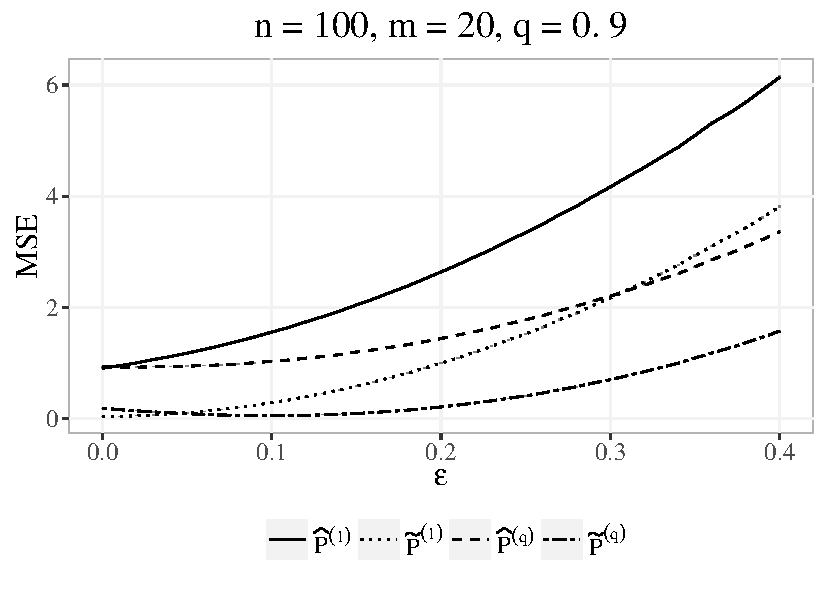
\includegraphics[width=1\textwidth]{./Figures/sim_eps.pdf}
\caption{Mean squared error in average by varying contamination ratio $\epsilon$ with fixed $n = 100$ and $m = 20$ based on 1000 Monte Carlo replicates, using $q=0.9$ when applying ML$q$E.
Different curves represent the simulated MSE associated with four different estimators.
1. MLE $\hat{P}^{(1)}$ vs ML$q$E $\hat{P}^{(q)}$:
MLE outperforms by a small amount when there is no contamination (i.e.\ $\epsilon = 0$), but it degrades dramatically when contamination probability increases;
2. MLE $\hat{P}^{(1)}$ vs ASE $\circ$ MLE $\widetilde{P}^{(1)}$: 
ASE procedure takes the low rank structure into account and $\widetilde{P}^{(1)}$ wins the bias-variance tradeoff;
3. ML$q$E $\hat{P}^{(q)}$ vs ASE $\circ$ ML$q$E $\widetilde{P}^{(q)}$: 
ML$q$E approximately preserves the low rank structure of the original graph, so ASE procedure still helps and $\widetilde{P}^{(q)}$ wins the bias-variance tradeoff;
4. ASE $\circ$ ML$q$E $\widetilde{P}^{(q)}$ vs ASE $\circ$ MLE $\widetilde{P}^{(1)}$: 
When contamination probability is large enough, $\widetilde{P}^{(q)}$ based on ML$q$E is better, since it inherits the robustness from ML$q$E.}
\label{fig:eps}
\end{figure}

Figure~\ref{fig:q} shows additional simulation results by varying the parameter $q$ in ML$q$E with fixed $n = 100$, $m = 20$ and $\epsilon = 0.1$ based on 1000 Monte Carlo replicates. 
%Different types of lines represent the simulated MSE associated with four different estimators. 
From the figure, we can see that the ASE procedure takes advantage of the graph structure and improves the performance of the corresponding estimators for a wide range of $q$. Moreover, for a wide range of $q$, the ML$q$E wins the bias-variance tradeoff and exhibits the robustness property compared to the MLE. And as $q$ goes to 1, ML$q$E goes to the MLE as expected.


\begin{figure}[!htb]
\centering
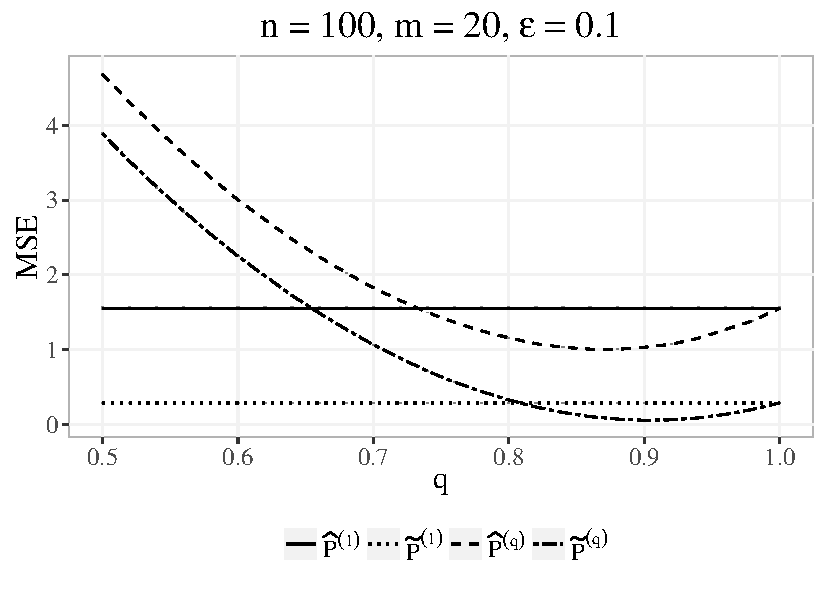
\includegraphics[width=1\textwidth]{./Figures/sim_q.pdf}
\caption{Mean squared error in average by varying the parameter $q$ in ML$q$E with fixed $n = 100$, $m = 20$ and $\epsilon = 0.1$ based on 1000 Monte Carlo replicates. Different curves represent the simulated MSE associated with the four different estimators.
1. ASE procedure takes advantage of the graph structure and improves the performance of the corresponding estimators independent of the selection of $q$;
2. Within a proper range of $q$, ML$q$E wins the bias-variance tradeoff and exibits robustness compared to the MLE. Also as $q$ goes to 1, ML$q$E goes to the MLE as expected.}
\label{fig:q}
\end{figure}


Figures \ref{fig:eps} and Figure~\ref{fig:q} provide a tangible demonstration of the theoretical results presented in Section~\ref{sec:robust_LLG_theoretical_result}.






\section{CoRR Brain Graphs Experiment}
\label{sec:robust_LLG_corr_data}

We now compare the four estimators on a structural connectomic dataset. The graphs in this dataset are based on diffusion tensor MR images. There are 114 different brain scans, each of which was processed to yield an undirected, weighted graph with no self-loops, using the m2g pipeline described in \citep{kiar2016ndmg}. The vertices of the graphs represent different regions in the brain defined according to an atlas. We used the Desikan atlas with 70 vertices in this experiment. The weight of an edge between two vertices represents the number of white-matter tracts connecting the corresponding two regions of the brain.

Generally, we do not expect the graphs to perfectly follow an RDPG, or even IEM. Before we perform our estimation, we will perform some exploratory analysis to check whether the data can reasonably be assumed to have approximate low-rank structure. Indeed, without at least approximately low-rank structure, we will not expect the ASE procedure to improve the bias-variance tradeoff because of a potential high bias. In the left panel of Figure~\ref{fig:screehist}, we plot the eigenvalues of the mean graph of all 114 graphs (with diagonal augmentation) in decreasing algebraic order for the Desikan atlases based on the m2g pipeline. The eigenvalues first decrease dramatically and then stay around 0 for a large range of dimensions. In addition, we also plot the histogram in the right panel of Figure~\ref{fig:screehist}. From the figure, we see that many eigenvalues are concentrated around zero. 
%In addition, we calculate the effective rank of $P$ to be 35 according to \citep{roy2007effective}. 
This exploration suggests that the information is mostly contained in the first few dimensions. Such approximate low-rank property provides an opportunity to win the bias-variance tradeoff by applying the ASE procedure.

\begin{figure}[!htbp]
\centering
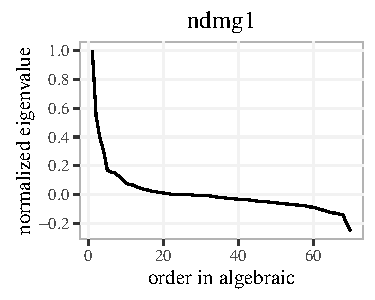
\includegraphics[height=.22\textheight]{./Figures/screeplot_m2g.pdf}
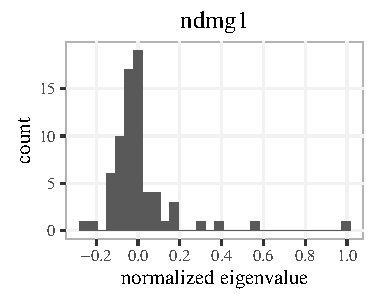
\includegraphics[height=.22\textheight]{./Figures/hist_m2g.pdf}
\caption{Screeplot and the histogram of the eigenvalues of the  mean of 114 graphs based on m2g pipeline.
The screeplot in the left panel shows the eigenvalues of the mean graph of all 114 graphs with diagonal augmentation in decreasing algebraic order for the Desikan atlas. The right panel shows the histogram of the eigenvalues of the mean graph of all 114 graphs with diagonal augmentation. Many eigenvalues are around zero, which lead to an approximate low-rank structure. 
%In addition, we calculate the effective rank of $P$ to be 35, which also suggests that the rank is relatively low.
}
\label{fig:screehist}
\end{figure}

We now discuss an important issue with respect to this current dataset. To compare the four estimators, we need a notion of the MSE, which requires the true parameter matrix $P$. However, unlike simulation experiment in Section~\ref{sec:sim_setting}, $P$ is definitely not available in practice since the 114 graphs themselves are also a sample from the population. We address this issue by finding a surrogate estimate for $P$ and using it to calculate the MSE.
%is a feasible way in this experiment. 
Recently, \citet{kiar2016ndmg} proposed a better pipeline ndmg2 compared to m2g. So the MLE derived from the 114 graphs in ndmg2 should be a relatively more accurate estimate of the actual probability matrix $P$ for the population. We use this as our surrogate for $P$ when calculating the MSE. However, such a $P$ generally has full rank, which breaks the low-rank assumptions. So this setting makes it hard for $\widetilde{P}^{(1)}$ and $\widetilde{P}^{(q)}$ to improve and is favorable to $\hat{P}^{(1)}$ and $\hat{P}^{(q)}$. Thus any improvement is conservative. Moreover, it is still possible that the 114 graphs from ndmg2 contain outliers. Thus by using the MLE of the ndmg2 data as $P$, the performance of ML$q$E-related estimators $\hat{P}^{(q)}$ and $\widetilde{P}^{(q)}$ are underestimated.
In summary, our approach to constructing a workable surrogate for $P$ relies on the availability of a better pipeline ndmg2, but is biased against both ASE-based and ML$q$E-based estimators; still, as we will see,  ASE $\circ$ ML$q$E is our winner.

In this experiment, we build the four estimates based on the sample of size $m$ from the m2g dataset, while using the MLE of all 114 graphs from the ndmg2 dataset as the surrogate probability matrix $P$. Note that diagonal augmentation procedure introduced in Section~\ref{sec:diag_aug} is also applied here to compensate for the unnecessary bias.
We run 100 simulations on this dataset for different sample sizes $m = 2, 5, 10$. Specifically, in each Monte Carlo replicate, we sample $m$ graphs out of the 114 from the m2g dataset and compute the four estimates based on the $m$ sampled graphs. Once again for simplicity, we set $q$ to be 0.9 without further exploration. However, the results are consistent for many choices of $q$. We then compare these estimates to the MLE of all 114 graphs in the ndmg2 dataset.
For the two low-rank estimators $\widetilde{P}^{(1)}$ and $\widetilde{P}^{(q)}$, we apply ASE into all possible dimensions, i.e.\ $d$ ranges from 1 to $n$. The MSE results are shown in Figure~\ref{fig:CCI}.

\begin{figure}
\centering
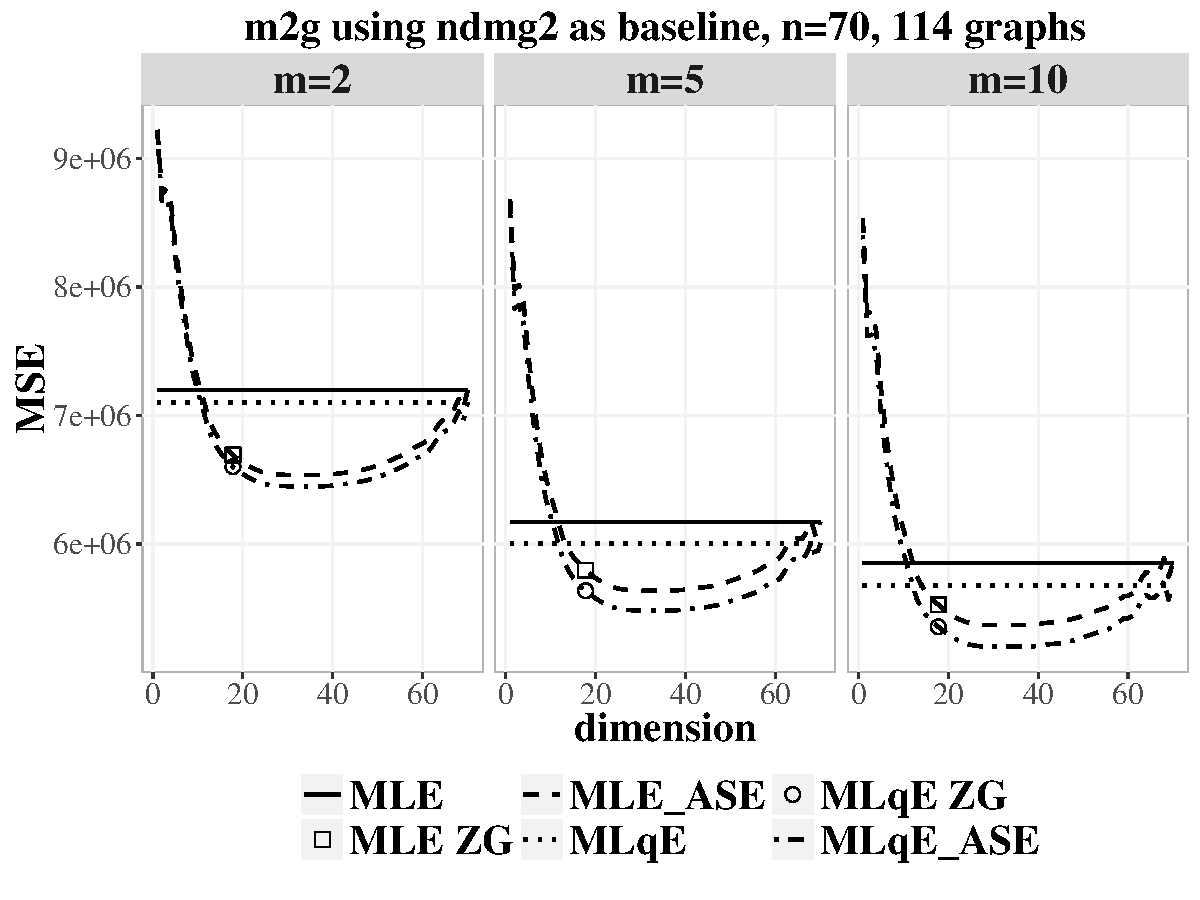
\includegraphics[width=\textwidth]{./Figures/CCI.pdf}
\caption{Comparison of MSE of the four estimators for the Desikan atlases at three sample sizes.
The x-axis represents the dimensions to embed while y-axis is the MSE of each estimator.
1. MLE $\hat{P}^{(1)}$ (horizontal solid line) vs MLqE $\hat{P}^{(q)}$ (horizontal dotted line):
ML$q$E outperforms MLE since in practice observations are always contaminated and robust estimators are preferred;
2. MLE $\hat{P}^{(1)}$ (horizontal solid line) vs ASE $\circ$ MLE $\widetilde{P}^{(1)}$ (dashed line):
$\widetilde{P}^{(1)}$ wins the bias-variance tradeoff when being embedded into a proper dimension; 
3. MLqE $\hat{P}^{(q)}$ (horizontal dotted line) vs ASE $\circ$ ML$q$E $\widetilde{P}^{(q)}$ (dashed dotted line):
$\widetilde{P}^{(q)}$ wins the bias-variance tradeoff when being embedded into an appropriate dimension; 
4.  ASE $\circ$ ML$q$E $\widetilde{P}^{(q)}$ (dashed dotted line) vs ASE $\circ$ MLE $\widetilde{P}^{(1)}$ (dashed line):
$\widetilde{P}^{(q)}$ is better, since it inherits the robustness from ML$q$E. The squares and circles represent the dimensions selected by the Zhu and Ghodsi method, which we see are reasonable choices. And more importantly, a wide range of dimensions lead to an improvement.
}
\label{fig:CCI}
\end{figure}


When $d$ is small, the ASE procedures underestimate the dimension and fail to capture important information, which leads to poor performance. In this work, we use Zhu and Ghodsi's method discussed in Section~\ref{sec:dim_select} to select the dimension $d$. We denote the selected dimensions by square and circle in the figure. We can see the algorithm performs adequately for selecting a dimension in which to embed. More importantly, there is a wide range of dimensions which lead to a better performance when applying ASE. Although the $P$ we are estimating is actually a high-rank matrix, ASE procedures still win the bias-variance tradeoff and improve performance even in this unfavorable setting.

Also, the robust estimator $\hat{P}^{(q)}$ performs relatively better than $\hat{P}^{(1)}$ in this experiment, even though $P$ still (presumably) contains outliers. This strongly indicates that there are many outliers in the original graphs from the m2g pipeline, and $\widetilde{P}^{(q)}$ successfully inherits the robustness from ML$q$E and outperforms $\widetilde{P}^{(1)}$.

For all three sample sizes ($m = 2, 5, 10$), $\widetilde{P}^{(q)}$ estimates $P$ most accurately while the target -- the surrogate $P$ -- is biased in favor of the other three estimators. As such, we expect $\widetilde{P}^{(q)}$ to provide an even better estimate for the true but unknown $P$.








\section{Proofs for Theory Results}
\label{sec:robust_LLG_proof}

\subsection{Outline of the Proofs}

Firstly, in Section~\ref{section:pf_MLqEvsMLE}, we prove in Lemma~\ref{lemma:ELqlEMLEproof} that when the contamination is large enough, the robust estimator $\hat{P}^{(q)}$ has smaller asymptotic bias compared to $\hat{P}^{(1)}$. By the results of minimum contrast estimator, we also show in Lemma~\ref{lemma:VarLqlVarMLEproof} that both estimators have variances going to zero as the number of graphs $m$ goes to infinity.

In Section~\ref{section:pf_MLEvsMLEASE1}, we analyze the properties of the ASE procedure. We first prove Theorem~\ref{thm:P1Diff}, which provides an upper bound for the spectral norm of the difference between the estimator $\hat{P}^{(1)}$ and its expectation $H_{ij}^{(1)} = E[\hat{P}_{ij}^{(1)}]$. Lemma~\ref{lemma:AlmostOrthogonalL1} shows that $U^{\top} \hat{U}$ can be approximated by an orthogonal matrix $W^{*} = W_1 W_2^{\top}$, where $U$ and $\hat{U}$ are the eigenspaces with respect to the largest $d$ eigenvalues of $H_{ij}^{(1)}$ and $\hat{P}^{(1)}$ respectively. More conveniently, Lemma~\ref{lemma:exchangeL1} indicates that we can change the order of $W^*$ in the matrix multiplications accordingly without affecting the result much. With these tool results, in Lemma~\ref{lemma:XhatDiffXWexpressionL1} we give an upper bound of $\|\hat{Z} - Z W\|_F$, which controls the error of the $\hat{Z}$ for estimating the true latent positions $Z$ up to orthogonal transformation.
% Briefly, in order to prove Lemma~\ref{lemma:XhatDiffXWexpressionL1}, we first write $\hat{Z} - U S^{1/2} W^*$ as the sum $(\hat{P} - H) U W^* \hat{S}^{-1/2} - U U^{\top}(\hat{P} - H)U W^*\hat{S}^{-1/2} + (I - U U^{\top})(\hat{P} - H) Q_3 \hat{S}^{-1/2} + Q_1 \hat{S}^{1/2} + U Q_2$, and bound each term accordingly based on Lemma~\ref{lemma:AlmostOrthogonalL1} and Lemma~\ref{lemma:exchangeL1}. Then by the Bernstein inequality, in Theorem~\ref{thm:XhatDiffXWL1} we give the bound of the ($2 \to \infty$)-norm of the $\hat{Z} - Z W$, i.e. $\max_i \| \hat{Z}_i - W Z_i \|_2$.
With the extent of Lemma~\ref{lemma:XhatDiffXWexpressionL1}, we then give a bound for the $2 \to \infty$-norm of $\hat{Z} - Z W$, i.e.\ we bound $\max_i \| \hat{Z}_i - W Z_i \|_2$ in Theorem~\ref{thm:XhatDiffXWL1}.

In Section~\ref{section:pf_MLEvsMLEASE2}, we give a bound of the estimation error $\left|  \hat{Z}_i^{\top} \hat{Z}_j - Z_i^{\top} Z_j \right|$ in Lemma~\ref{lemma:1stMomentPhatDiffL1} based on the results in Section~\ref{section:pf_MLEvsMLEASE1}. In order to bound the variance of our estimator $\widetilde{P}^{(1)}$, all results in this section will be based on a truncated version of $\widetilde{P}^{(1)}$ defined in Definition~\ref{def:truncationMLE}. This is purely for technical reasons and will not affect the estimation procedure in practice, which is discussed in details in Remark~\ref{remark:truncation}. We then bound the expectation (Lemma~\ref{lm:L1Consistentproof}) and variance (Theorem~\ref{thm:VarASEL1proof}) of $\widetilde{P}^{(1)}$ by carefully choosing a truncation point $a$ and applying the above truncation argument. As a direct result, we obtain the bound for the relative efficiency between $\hat{P}_{ij}^{(1)}$ and $\widetilde{P}_{ij}^{(1)}$ in Theorem~\ref{thm:AREL1proof}.

In Section~\ref{section:pf_MLqEASEvsMLqE}, we compare the performance between $\widetilde{P}^{(q)}$ and $\hat{P}^{(q)}$. The results in this section are proved in a similar manner to those in Section~\ref{section:pf_MLEvsMLEASE1} and Section~\ref{section:pf_MLEvsMLEASE2}. However, since the ML$q$E estimator for a mixture distribution model does not have a closed form expression, we explore a relationship between MLE and ML$q$E to bound $\widetilde{P}^{(q)}$ and $\hat{P}^{(q)}$; this technique could be of independent interest. Finally, in Section~\ref{section:MLqEASEvsMLEASE}, we compare the performance between $\widetilde{P}^{(q)}$ and $\widetilde{P}^{(1)}$.

In Section~\ref{section:pf_other}, we provide proofs for all supplementary results mentioned in the manuscript.

Before presenting the proofs, we first define the following notion of ``with high probability'' that is used throughout this work.
\begin{definition}
We say a bound holds with high probability, if there exits a constant $n_0(c)$ such that if $n > n_0$, then for any $\eta$ satisfying $n^{-c} < \eta < 1/2$, the bound holds with probability greater than $1 - \eta$.
\end{definition}

\subsection{$\hat{P}^{(q)}$ vs. $\hat{P}^{(1)}$}
\label{section:pf_MLqEvsMLE}

\begin{lemma}
\label{lemma:LqlMLE}
Let $X_1, \cdots, X_m \stackrel{iid}{\sim} \mathrm{Exp}(P)$ with $m \ge 2$ and $E[X_1] = P$. Then with probability $1$,
%Given any observation $x = (x_1, \cdots, x_m)$ of $X_1, X_2, \dots, X_m$ such that $x_{(1)} > 0$ and not all $x_i$'s are the same, then no matter how the data is sampled, we have
\begin{itemize}
\item There exists at least one solution to the ML$q$ equation;
\item All the solutions to the ML$q$ equation are less than the MLE.
\end{itemize}
Thus the ML$q$E $\hat{P}^{(q)}$, the root closest to the MLE, is well defined.
\end{lemma}
\begin{proof}
Let $x_1, \cdots, x_m$ be the observed values of $X_1, X_2, \dots, X_m$. Then with probability $1$, the $x_i$ are unique and $x_{(1)} = \min_{i} x_i > 0$. The MLE is
\[
	\hat{P}^{(1)}(x) = \bar{x}.
\]

Let $g(\theta, x) = \sum_{i=1}^m e^{-\frac{(1-q)x_i}{\theta}}(x_i - \theta)$. Then the ML$q$ equation is $g(\theta, x) = 0$. Now let $l$ be the smallest index such that $x_{(1)} \le \cdots \le x_{(l)} \le \bar{x} \le x_{(l+1)} \le \cdots$. Define $s_i = \bar{x} - x_{(i)}$ for $1 \le i \le l$, and $t_{i} = x_{(l+i)} - \bar{x}$ for $1 \le i \le m - l$. Note that $\sum_{i=1}^l s_i = \sum_{i=1}^{m-l} t_i$. Then for any $\theta \ge \bar{x}$, we have
\begin{align*}
g(\theta, x) & = \sum_{i=1}^m e^{-\frac{(1-q)x_{(i)}}{\theta}}(x_{(i)} - \theta)
= \sum_{i=1}^m e^{-\frac{(1-q)x_{(i)}}{\theta}}(x_{(i)} - \bar{x} + \bar{x} - \theta) \\
& = - \sum_{i=1}^l e^{-\frac{(1-q)x_{(i)}}{\theta}}s_i
+ \sum_{i=1}^{m-l} e^{-\frac{(1-q)x_{(i+l)}}{\theta}}t_i
+ \sum_{i=1}^m e^{-\frac{(1-q)x_{(i)}}{\theta}}(\bar{x} - \theta)\\
& \le - \sum_{i=1}^l e^{-\frac{(1-q)x_{(i)}}{\theta}}s_i
+ \sum_{i=1}^{m-l} e^{-\frac{(1-q)x_{(i+l)}}{\theta}}t_i \\
& \le - e^{-\frac{(1-q)x_{(l+1)}}{\theta}} \sum_{i=1}^l s_i
+ \sum_{i=1}^{m-l} e^{-\frac{(1-q)x_{(i+l)}}{\theta}}t_i \\
& \le - e^{-\frac{(1-q)x_{(l+1)}}{\theta}} \sum_{i=1}^{m-l} t_i
+ \sum_{i=1}^{m-l} e^{-\frac{(1-q)x_{(i+l)}}{\theta}}t_i \\
& \le - \sum_{i=1}^{m-l} e^{-\frac{(1-q)x_{(i+l)}}{\theta}}t_i
+ \sum_{i=1}^{m-l} e^{-\frac{(1-q)x_{(i+l)}}{\theta}}t_i\\
& = 0,
\end{align*}
and equality holds if and only if all $x_i$'s are the same, which occurs with probability $0$. Thus with probablity $1$, $g(\theta, x) < 0$ for all $\theta \ge \bar{x}$.

Denote any solution to the ML$q$E equation as $\hat{P}^{(q)}(x)$; we then have that
\begin{itemize}
\item $g(\hat{P}^{(q)}(x), x) = 0$;
\item $\lim_{\theta \rightarrow 0^+}g(\theta, x) = 0$;
\item $g(\theta, x) > 0$ when $\theta < x_{(1)}$;
\end{itemize}

Thus there exists at least one solution to the ML$q$E equation. And since all solutions to the ML$q$E equation are in the interval $(x_{(1)},\bar{x})$, we have t$\hat{P}^{(q)}(x) \leq \hat{P}^{(1)}(x)$.
\end{proof}

\begin{lemma}
\label{lemma:PopulationLqExist}
Consider an exponential distribution model while the data is actually sampled from the contaminated model $X, X_1, \cdots, X_m \stackrel{iid}{\sim} (1-\epsilon) \mathrm{Exp}(P) + \epsilon \mathrm{Exp}(C)$. Denote such contaminated distribution as $F$.
Then there exists exactly one real solution $\theta(F)$ of the population version of ML$q$ equation,
i.e.\ $E_F[e^{-\frac{(1-q)X}{\theta(F)}}(X - \theta(F))] = 0$. Moreover, $\theta(F) < E_F[\bar{X}] = (1-\epsilon) P + \epsilon C$.
\end{lemma}
\begin{proof}
For the MLE, i.e.\ $\bar{X}$, we have $E[\bar{X}] = (1-\epsilon) P + \epsilon C$.
According to Equation (3.2) in \citep{ferrari2010maximum}, $\theta(F)$ satisfies
\[
\frac{\epsilon C}{(C(1-q) + \theta)^2} - \frac{\epsilon}{C(1-q) + \theta}
+\frac{(1-\epsilon) P}{(P(1-q) + \theta)^2} - \frac{(1-\epsilon)}{P(1-q) + \theta}
= 0,
\]
i.e.\
\[
\frac{\epsilon (\theta - Cq)}{(C(1-q) + \theta)^2} =
\frac{(1-\epsilon) (P q - \theta)}{(P(1-q) + \theta)^2}.
\]
Define $h(\theta) = (C(1-q) + \theta)^2 (1-\epsilon) (P q - \theta) - (P(1-q) + \theta)^2 \epsilon (\theta - Cq)$.
Then $\lim_{\theta \to \infty}h(\theta) = -\infty$, $h(0) > 0$, and $h(Cq) < 0$.
Consider $q$ as the variable and solve the equation $h(E[\bar{X}]) = 0$, we have three roots and one of them is $q = 1$ obviously.
The other two roots are
\[
\frac{(P + C)\left( (P-C)^2 \epsilon(1-\epsilon) + 2PC \right)}{2PC(P \epsilon + C(1-\epsilon))}
\pm \sqrt{\frac{\epsilon(1-\epsilon)(C-P)^2\left(\epsilon(1-\epsilon)(C-P)^4 - 4P^2C^2\right)}{4 P^2 C^2 (P\epsilon + C(1-\epsilon))^2}}.
\]
To prove the roots are greater or equal to 1, we need to show
\[
\frac{(P + C)\left( (P-C)^2 \epsilon(1-\epsilon) + 2PC \right)}{2PC(P \epsilon + C(1-\epsilon))}
- \sqrt{\frac{\epsilon(1-\epsilon)(C-P)^2\left(\epsilon(1-\epsilon)(C-P)^4 - 4P^2C^2\right)}{4 P^2 C^2 (P\epsilon + C(1-\epsilon))^2}} > 1.
\]
For the first part,
\[
\frac{(P + C)\left( (P-C)^2 \epsilon(1-\epsilon) + 2PC \right)}{2PC(P \epsilon + C(1-\epsilon))}\\
> 1 + \frac{(P-C)^2 \epsilon (1-\epsilon) (P+C)}{2PC(P \epsilon + C(1-\epsilon))}.
\]
To prove the roots are greater or equal to 1, we just need to show
\[
(P-C)^4 \epsilon^2 (1-\epsilon)^2 (P+C)^2 \ge \epsilon^2(1-\epsilon)^2(C-P)^6.
\]
Then it is sufficient to show that
\[
(P+C)^2 \ge (C-P)^2,
\]
which is true.
Combined with the fact that when $q = 0$, $h(E[\bar{X}]) < 0$, we have for any $0 < q < 1$, $h(E[\bar{X}]) < 0$.

The equation $h(\theta) = 0$ is a cubic polynomial, so it has at most three real roots. In addition, by calculating we know there is only one real root, while the other two are complex roots. Combined with the fact that $h(P q) > 0$, we have for any $0 < q < 1$, the only real root of the population version of ML$q$ equation is less than $E[\bar{X}] = (1-\epsilon)P + \epsilon C$.
\end{proof}

\begin{lemma}[Theorem~\ref{thm:MLEvsMLqE}]
\label{lemma:ELqlEMLEproof}
For any $0 < q < 1$, there exists $C_0(P_{ij}, \epsilon, q) > 0$ such that under the contaminated model with $C > C_0(P_{ij}, \epsilon, q)$,
\[
	\lim_{m \to \infty} \left| E[\hat{P}^{(q)}_{ij}] - P_{ij} \right| < 
    \lim_{m \to \infty} \left| E[\hat{P}^{(1)}_{ij}] - P_{ij} \right|,
\]
for $1 \le i, j \le n$ and $i \ne j$.
\end{lemma}
\begin{proof}
For the MLE $\hat{P}^{(1)}_{ij} = \bar{A}_{ij}$,
\[
	E[\hat{P}^{(1)}_{ij}] = E[\bar{A}_{ij}]
    = \frac{1}{m} \sum_{t = 1}^m E[A_{ij}^{(t)}]
    = E[A_{ij}^{(1)}]
    = (1-\epsilon) P_{ij} + \epsilon C_{ij}.
\]
As shown in Lemma \ref{lemma:PopulationLqExist}, $\theta(F)$ satisfies
\[
\frac{\epsilon (\theta(F) - C_{ij}q)}{(C_{ij}(1-q) + \theta(F))^2} =
\frac{(1-\epsilon) (P_{ij} q - \theta(F))}{(P_{ij}(1-q) + \theta(F))^2}.
\]
Thus $\theta(F) - C_{ij} q$ and $\theta(F) - P_{ij} q$ should have different signs. Combined with $C_{ij} > P_{ij}$, we have
\[
q P_{ij} < \theta(F).
\]
To have a smaller asymptotic bias in absolute value, combined with Lemma \ref{lemma:ELqConverge}, we need
\[
|\theta(F) - P_{ij}| < \epsilon (C_{ij} - P_{ij}).
\]
Based on Lemma \ref{lemma:LqlMLE}, we need
\[
q P_{ij} > P_{ij} - \epsilon(C_{ij} - P_{ij}),
\]
i.e.
\[
C_{ij} > P_{ij} + \frac{(1-q) P_{ij}}{\epsilon} = C_0(P_{ij}, \epsilon, q).
\]
\end{proof}


\begin{lemma}
\label{lemma:minimumcontrast}
The ML$q$E based on the model to be exponential distribution $\mathrm{Exp}(P)$ while the data is actually sampled from the contaminated distribution $(1-\epsilon) \mathrm{Exp}(P) + \epsilon \mathrm{Exp}(C)$ is a minimum contrast estimator.
\end{lemma}
\begin{proof}
Consider the contaminated distribution $F(x) = (1-\epsilon) f(x; P) + \epsilon f(x; C)$, where $f(x)$ represents the pdf of exponential distribution. By Lemma~\ref{lemma:PopulationLqExist}, we know there is a one-to-one correspondence between the uncontaminated parameter $P$ and the only real solution $\theta(F)$ of the population version of ML$q$ equation,
i.e.\ $E_F[e^{-\frac{(1-q)X}{\theta(F)}}(X - \theta(F))] = 0$. Let $r(\theta(F)) = P$.
Then we can define $\rho(x; \theta) = \frac{f(x; r(\theta))^{1-q}}{1 - q}$, where $q \in (0, 1)$ is a constant.
By reparameterizing $\rho(x; \theta)$ to $\widetilde{\rho}(x; r)$ such that $\widetilde{\rho}(x; r(\theta)) = \rho(x; \theta)$, we can use the proof of Lemma~\ref{lemma:PopulationLqExist} directly to prove that $D(\theta_0, \theta) = E_{\theta_0}[\rho(X, \theta)]$ is uniquely minimized at $\theta_0$. Thus the ML$q$E is a minimum contrast estimator.
\end{proof}

\begin{lemma}
\label{lemma:UniformConvergence}
Uniform convergence of the MLq equation, i.e.\
\[
	\sup_{\theta \in [0, R]} \left| \frac{1}{m} \sum_{i=1}^m e^{-\frac{(1-q) X_i}{\theta}}(X_i - \theta) - E_F[e^{-\frac{(1-q) X}{\theta}}(X - \theta)] \right| \stackrel{a.s.}{\to} 0.
\]
\end{lemma}
\begin{proof}
Define $g(x,\theta) = e^{-\frac{(1-q) x}{\theta}}(x - \theta)$ and $d(x) = e^{-\frac{(1-q)x}{R}}(x + R)$. Then $E_F[d(X)] < \infty$ and $g(x,\theta) \le d(x)$ for all $\theta \in [0, R]$.
Combined with the fact that $[0, R]$ is compact and the function $g(x,\theta)$ is continuous at each $\theta$ for all $x > 0$ and measurable function of $x$ at each $\theta$, we have the uniform convergence by Lemma 2.4 in \citep{newey1994large}.
\end{proof}

\begin{lemma}
\label{lemma:ELqConverge}
$\hat{P}_{ij}^{(q)} \stackrel{P}{\to} \theta(F_{ij})$ as $m \to \infty$, where $F_{ij}$ is the contaminated distribution $(1-\epsilon) \mathrm{Exp}(P_{ij}) + \epsilon \mathrm{Exp}(C_{ij})$, and $ \theta(F_{ij})$ is defined in Lemma~\ref{lemma:PopulationLqExist}. 
\end{lemma}
\begin{proof}
By the proof of Lemma~\ref{lemma:PopulationLqExist}, we have
\[
	\inf\{D(\theta_0, \theta): |\theta - \theta_0| \ge \epsilon \} > D(\theta_0, \theta_0)
\]
for every $\epsilon > 0$. Combined with Lemma~\ref{lemma:UniformConvergence}, we know the ML$q$ is consistent based on Theorem 5.2.3 in \citep{bickel2007mathematical}.
\end{proof}

\begin{lemma}[Theorem~\ref{thm:MLEvsMLqE}]
\label{lemma:VarLqlVarMLEproof}
For $1 \le i, j \le n$, 
\[
	\mathrm{Var}(\hat{P}^{(1)}_{ij})
    = \mathrm{Var}(\hat{P}^{(q)}_{ij}) = O(1/m).
\]
And thus
\[
	\lim_{m \to \infty} \mathrm{Var}(\hat{P}^{(1)}_{ij})
    = \lim_{m \to \infty} \mathrm{Var}(\hat{P}^{(q)}_{ij}) = 0.
\]
\end{lemma}
\begin{proof}
Both MLE and ML$q$E are minimum constrast estimators. By consistency (shown in Lemma~\ref{lemma:ELqConverge}) and other regularity conditions, we know the variances are both of order $1/m$ based on Theorem 5.4.2 in \citep{bickel2007mathematical}.
\end{proof}



\subsection{ASE Procedure of $\hat{P}^{(1)}$}
\label{section:pf_MLEvsMLEASE1}

\begin{theorem}%[Theorem 3.3]
\label{thm:P1Diff}
Let $P$ and $C$ be two $n$-by-$n$ symmetric matrices satisfying element-wise conditions $0 < P_{ij} \le C_{ij} \le R$ for some constant $R > 0$. For $0 < \epsilon < 1$, we define $m$ symmetric and hollow matrices as
\[
	A^{(t)} \stackrel{iid}{\sim} (1-\epsilon) \mathrm{Exp}(P) + \epsilon \mathrm{Exp}(C),
\]
for $1 \le t \le m$.
Let $\hat{P}^{(1)}$ be the element-wise MLE based on exponential distribution with $m$ observations.
Define $H_{ij}^{(1)} = E[\hat{P}_{ij}^{(1)}] = (1-\epsilon) P_{ij} + \epsilon C_{ij}$,
then for any constant $c > 0$, there exists another constant $n_0(c)$, independent of $n$, $P$, $C$ and $\epsilon$, such that if $n > n_0$, then for all $\eta$ satisfying $n^{-c} \le \eta \le 1/2$,
\[
	P \left( \| \hat{P}^{(1)} - H^{(1)} \|_2 \le 4 R \sqrt{n \ln(n/\eta)/m}\right) \ge 1 - \eta.
\]
\end{theorem}
\textbf{Remark:} This is an extended version of Theorem 3.1 in \citep{oliveira2009concentration}. \\
\begin{proof}
Let $\{e_i\}_{i=1}^n$ be the canonical basis for $\mathbb{R}^n$. For each $1 \le i, j \le n$, define a corresponding matrix $G_{ij}$:
\[
    G_{ij} \equiv \left\{
    \begin{array}{l l}
        e_i e_j^{\top} + e_j e_i^{\top}, \quad & i \ne j;\\
        e_i e_i^{\top}, \quad & i = j.
    \end{array}
    \right.
\]
Thus
\[
\hat{P}^{(1)} = \sum_{1 \le i < j \le n} \hat{P}^{(1)}_{ij} G_{ij} = \frac{1}{m}\sum_{t=1}^m \sum_{1 \le i < j \le n} A^{(t)}_{ij} G_{ij}
\]
and
\[
H^{(1)} = \sum_{1 \le i < j \le n} H^{(1)}_{ij} G_{ij}.
\]
Then we have $\hat{P}^{(1)} - H^{(1)} = \frac{1}{m} \sum_{1 \le t \le m, 1 \le i < j \le n} X_{ij}^{(t)}$, where $X_{ij}^{(t)} = \left( A^{(t)}_{ij} - H^{(1)}_{ij} \right) G_{ij}$ for $1 \le t \le m$ and $1 \le i < j \le n$.

First bound the $k$-th moment of $X_{ij}$ for $1 \le i < j \le n$ as follows:
\begin{align*}
	E[(A^{(t)}_{ij} - H^{(1)}_{ij})^k]
    \le & (1-\epsilon) \cdot \exp(-H_{ij}/P_{ij}) P_{ij}^k \Gamma(1+k, -H_{ij}/P_{ij}) \\
    & + \epsilon \cdot \exp(-H_{ij}/C_{ij}) C_{ij}^k \Gamma(1+k, -H_{ij}/C_{ij}) \\
    \le & \left( (1-\epsilon) \cdot \exp(-H_{ij}/P_{ij}) P_{ij}^k + \epsilon \cdot \exp(-H_{ij}/C_{ij}) C_{ij}^k \right) k! \\
    \le & \left( (1-\epsilon) \cdot P_{ij}^k + \epsilon \cdot C_{ij}^k \right) k! \\
    \le & R^k k!,
    \stepcounter{equation}\tag{\theequation}\label{eqn:expectpdiffqpowerkL1}
\end{align*}

Combined with
\[
    G_{ij}^k \equiv \left\{
    \begin{array}{l l}
        e_i e_i^{\top} + e_j e_j^{\top}, \quad & $k$ \text{ is even};\\
        e_i e_j^{\top} + e_j e_i^{\top}, \quad & $k$ \text{ is odd},
    \end{array}
    \right.
\]
thus we have
\begin{enumerate}
\item When $k$ is even,
\[
E[(X_{ij}^{(t)})^k] = E[(A^{(t)}_{ij} - H^{(1)}_{ij})^k] G_{ij}^2 \preceq k! R^k G_{ij}^2;
\]
\item When $k$ is odd,
\[
E[(X_{ij}^{(t)})^k] = E[(A^{(t)}_{ij} - H^{(1)}_{ij})^k] G_{ij} \preceq k! R^k G_{ij}^2.
\]
\end{enumerate}
So
\[
E[(X_{ij}^{(t)})^k] \preceq k! R^k G_{ij}^2.
\]
Let
\[
	\sigma^2 := \left\| \sum_{1 \le t \le m, 1 \le i < j \le n} (\sqrt{2} R G_{ij})^2 \right\|_2 = 2 R^2 m \| (n - 1) I \|_2 = 2 R^2 m (n - 1).
\]
Notice that random matrices $X_{ij}^{(t)}$ are independent, self-adjoint and have mean zero, apply Theorem 6.2 in \citep{tropp2012user} we have
\begin{align*}
	P \left( \lambda_{\max}(\hat{P}^{(1)} - H^{(1)}) \ge t \right)
	& = P \left( \lambda_{\max}\left(\frac{1}{m} \sum_{1 \le t \le m, 1 \le i < j \le n} X_{ij}^{(t)}\right) \ge t \right) \\
	& = P \left( \lambda_{\max}\left(\sum_{1 \le t \le m, 1 \le i < j \le n} X_{ij}^{(t)}\right) \ge m t \right) \\
	& \le n \exp \left( - \frac{(m t)^2/2}{\sigma^2 + R m t} \right) \\
	& \le n \exp \left( - \frac{m t^2/2}{2 R^2 n + R t} \right).
\end{align*}

Now consider $Y_{ij}^{(t)} \equiv \left( H_{ij}^{(1)} - A_{ij}^{(t)} \right) G_{ij}$, for $1 \le t \le m$ and $1 \le i < j \le n$. Then we have $H^{(1)} - \hat{P}^{(1)} = \frac{1}{m} \sum_{1 \le t \le m, 1 \le i < j \le n} Y_{ij}^{(t)}$.
Since
\[
	E[(H^{(1)} - \hat{P}^{(1)})^k]
    = (-1)^k E[(\hat{P}^{(1)} - H^{(1)})^k],
\]
\begin{enumerate}
\item When $k$ is even,
\[
E[(Y_{ij}^{(t)})^k] = E[(\hat{P}^{(1)} - H^{(1)})^k] G_{ij}^2 \preceq k! R^k G_{ij}^2;
\]
\item When $k$ is odd,
\[
E[Y_{ij}^k] = - E[(\hat{P}^{(1)} - H^{(1)})^k] G_{ij} \preceq k! R^k G_{ij}^2.
\]
\end{enumerate}
Thus by similar arguments,
\begin{align*}
	P \left( \lambda_{\min}(\hat{P}^{(1)} - H^{(1)}) \le -t \right) &
    = P \left( \lambda_{\max}(H^{(1)} - \hat{P}^{(1)}) \ge t \right) \\
    & \le n \exp \left( - \frac{m t^2/2}{2 R^2 n + R t} \right).
\end{align*}
Therefore we have
\[
	P \left( \| \hat{P}^{(1)} - H^{(1)} \|_2 \ge t \right)
    \le n \exp \left( - \frac{m t^2/2}{2 R^2 n + R t} \right).
\]

Now let $c > 0$ be given and assume $n^{-c} \le \eta \le 1/2$. Then there exists a $n_0(c)$ independent of $n$, $P$, $C$ and $\epsilon$ such that whenever $n > n_0(c)$,
\[
	t =  4 R \sqrt{n \ln(n/\eta)/m} \le 6 R n.
\]

Plugging this $t$ into the equation above, we get
\[
	P(\| \hat{P}^{(1)} - H^{(1)} \|_2 \ge 4 R \sqrt{n \ln(n/\eta)/m})
    \le n \exp\left(-\frac{t^2}{16 R^2 n}\right) = \eta.
\]
\end{proof}

Define $H^{(1)} = E[\hat{P}^{(1)}] = (1-\epsilon) P + \epsilon C$, where $P = X X^{\top}$, $X \in \mathbb{R}^{n \times d}$, $C = Y Y^{\top}$, $Y \in \mathbb{R}^{n\times d'}$.
Let $d^{(1)} = \mathrm{rank}(H^{(1)})$ be the dimension in which we are going to embed $\hat{P}^{(1)}$. Then we can define $H^{(1)} = Z Z^{\top}$ where $Z \in \mathbb{R}^{n \times d^{(1)}}$.
Since $H^{(1)} = [\sqrt{1-\epsilon} X, \sqrt{\epsilon} Y] [\sqrt{1-\epsilon} X, \sqrt{\epsilon} Y]^{\top}$, we have $d^{(1)} \le d+d'$.


For simplicity, from now on, we will use $\hat{P}$ to represent $\hat{P}^{(1)}$, use $H$ to represent $H^{(1)}$ and use $k$ to represent the dimension $d^{(1)}$ we are going to embed. Assume $H = U S U^{\top} = Z Z^{\top}$, where $Z = [Z_1, \cdots, Z_n]^{\top}$ is a $n$-by-$k$ matrix. Then our estimate for $Z$ up to rotation is $\hat{Z} = \hat{U} \hat{S}^{1/2}$, where $\hat{U} \hat{S} \hat{U}^{\top}$ is the rank-$k$ spectral decomposition of $|\hat{P}| = (\hat{P}^{\top} \hat{P})^{1/2}$.

Furthermore, we assume that the second moment matrix $E[Z_1 Z_1^{\top}]$ is rank $k$ and has distinct eigenvalues $\lambda_i(E[Z_1 Z_1^{\top}])$. In particular, we assume that there exists $\delta > 0$ such that
\[
	\delta < \lambda_k(E[Z_1 Z_1^{\top}])
\]

\begin{lemma}
\label{lemma:eigSShatL1}
Under the above assumptions, $\lambda_i(H) = \Theta(n)$ with high probability when $i \le k$, i.e.\ the largest $k$ eigenvalues of $H$ is of order $n$. Moreover, we have $\| S \|_2 = \Theta(n)$ and $\| \hat{S} \|_2 = \Theta(n)$ with high probability.
\end{lemma}
\textbf{Remark:} This is an extended version of Proposition 4.3 in \citep{sussman2014consistent}. \\
\begin{proof}
Note that $\lambda_i(H) = \lambda_i(Z Z^{\top}) = \lambda_i(Z^{\top} Z)$ when $i \le k$. Since each entry of $Z^{\top} Z$ is a sum of $n$ independent random variables each in $[0, R]$, i.e. $(Z^{\top} Z)_{ij} = \sum_{l = 1}^n Z_{li} Z_{lj}$.
By Hoeffding's inequality,
\[
P(|(Z^{\top} Z - n E[Z_1 Z_1^{\top}])_{ij}| \ge t) \le 2 \exp(-\frac{2t^2}{n R^2}).
\]
Now let $c > 0$ and assume $n^{-c} \le \eta \le 1/2$. Let
\[
	t =  R \sqrt{n \ln(\sqrt{2/\eta})},
\]
we have
\[
P\left(|(Z^{\top} Z - n E[Z_1 Z_1^{\top}])_{ij}| \ge R \sqrt{n \ln(\sqrt{2/\eta})}\right) \le \eta.
\]
By the union bound, we have
\[
P\left(\|Z^{\top} Z - n E[Z_1 Z_1^{\top}]\|_F \ge k R \sqrt{n \ln(\sqrt{2/\eta})}\right) \le k^2 \eta.
\]

Then by Weyl's Theorem \citep{horn2012matrix}, we have
\[
|\lambda_i(H) - n \lambda_i(E[Z_1 Z_1^{\top}])| \le \|Z^{\top} Z - n E[Z_1 Z_1^{\top}]\|_2 = O(\sqrt{n\log{(1/\eta)}})
\]
with probability at least $1 - k^2 \eta$.
Thus $\lambda_i(H) = S_{ii} = \Theta(n)$ with probability at least $1 - \frac{2 k^2}{n^2}$ when $i \le k$.
Moreover,
\[
\| H \|_2 - \|H - \hat{P}\|_2 \le \|\hat{S}\|_2 \le \|\hat{P} - H\|_2 + \|H\|_2.
\]
Combined with Theorem \ref{thm:P1Diff}, with high probability we have $\|\hat{S}\|_2 = \Theta(n)$.
\end{proof}

\begin{lemma}
\label{lemma:AlmostOrthogonalL1}
Let $W_1 \Sigma W_2^{\top}$ be the singular value decomposition of $U^{\top} \hat{U}$. Then for sufficiently large $n$, 
\[
	\| U^{\top} \hat{U} - W_1 W_2^{\top} \|_F = O(m^{-1} n^{-1} \log n)
\]
with high probability.
\end{lemma}
\begin{proof}
Let $\sigma_1, \cdots, \sigma_k$ denote the singular values of $U^{\top} \hat{U}$. Then $\sigma_i = \cos(\theta_i)$ where the $\theta_i$ are the principal angles between the subspaces spanned by $\hat{U}$ and $U$. Furthermore, by the Davis-Kahan $\sin(\Theta)$ theorem \citep{davis1970rotation}, combined with Theorem \ref{thm:P1Diff} and Lemma \ref{lemma:eigSShatL1},
\begin{equation}
\label{eqn:uhat2u2diffL1}
\begin{split}
	& \|\hat{U} \hat{U}^{\top} - U U^{\top}\|_2 = \max_i |\sin(\theta_i)| \\
    \le & \frac{\|\hat{P} - H\|_2}{\lambda_k(H)}
    \le \frac{C \sqrt{n \log n/m}}{n} \\
    = & O(m^{-1/2} n^{-1/2} \sqrt{\log n})
\end{split}
\end{equation}
for sufficiently large $n$ with high probability. Here $\lambda_k(H)$ denotes the $k$-th largest eigenvalue of $H$.
Thus with high probability, 
\begin{align*}
	\| U^{\top} \hat{U} - W_1 W_2^{\top} \|_F
    & = \| \Sigma - I \|_F
    = \sqrt{\sum_{i=1}^k (1-\sigma_i)^2} \\
    & \le \sum_{i=1}^k (1-\sigma_i) \le \sum_{i=1}^k (1-\sigma_i^2) \\
    & = \sum_{i=1}^k \sin^2(\theta_i)
    \le k \|\hat{U} \hat{U}^{\top} - U U^{\top}\|_2^2 \\
    & = O(m^{-1} n^{-1} \log n).
\end{align*}
\end{proof}

We will denote the orthogonal matrix $W_1 W_2^{\top}$ by $W^*$.

\begin{lemma}
\label{lemma:exchangeL1}
For sufficiently large $n$,
\[
	\| W^* \hat{S} - S W^* \|_F = O(m^{-1/2} \log n),
\]
\[
	\|W^* \hat{S}^{1/2} - S^{1/2} W^* \|_F = O(m^{-1/2} n^{-1/2} \log n)
\]
and
\[
	\| W^* \hat{S}^{-1/2} - S^{-1/2} W^* \|_F = O(m^{-1/2} n^{-3/2} \log n)
\]
with high probability.
\end{lemma}
\begin{proof}
By Proposition~2.1 in \citep{rohe2011spectral} and Equation~(\ref{eqn:uhat2u2diffL1}), we have for some orthogonal matrix $W$, 
\begin{align*}
& \|\hat{U} - U W\|_F^2 \le \frac{2 \|\hat{U} \hat{U}^{\top} - U U^{\top}\|_F^2}{\delta^2}
\le \frac{8 k^2 \|\hat{U} \hat{U}^{\top} - U U^{\top}\|_2^2}{\delta^2} \\
= & O(m^{-1} n^{-1} \log n),
\end{align*}
with high probability.
Let $Q = \hat{U} - U U^{\top} \hat{U}$. And $Q$ is the residual after projecting $\hat{U}$ orthogonally onto the column space of $U$, we have
\begin{equation}
\label{eqn:QFnormL1}
\| Q \|_F = \| \hat{U} - U U^{\top} \hat{U} \|_F \le \| \hat{U} - U T \|_F = O(m^{-1/2} n^{-1/2} \sqrt{\log n}).
\end{equation}
for all $k \times k$ matrices $T$ with high probability. 
Then
\begin{align*}
	W^* \hat{S} = & (W^* - U^{\top} \hat{U}) \hat{S} + U^{\top} \hat{U} \hat{S}
    = (W^* - U^{\top} \hat{U}) \hat{S} + U^{\top} \hat{P} \hat{U} \\
    = & (W^* - U^{\top} \hat{U}) \hat{S} + U^{\top} (\hat{P} - H) \hat{U} + U^{\top} H \hat{U} \\
    = & (W^* - U^{\top} \hat{U}) \hat{S} + U^{\top} (\hat{P} - H) Q + U^{\top} (\hat{P} - H) U U^{\top} \hat{U} + U^{\top} H \hat{U} \\
    = & (W^* - U^{\top} \hat{U}) \hat{S} + U^{\top} (\hat{P} - H) Q + U^{\top} (\hat{P} - H) U U^{\top} \hat{U} + S U^{\top} \hat{U}.
\end{align*}
Combined with Theorem~\ref{thm:P1Diff}, Lemma~\ref{lemma:eigSShatL1}, Lemma~\ref{lemma:AlmostOrthogonalL1}, we have
\begin{align*}
	& \| W^* \hat{S} - S W^* \|_F \\
    = & \| (W^* - U^{\top} \hat{U}) \hat{S} + U^{\top} (\hat{P} - H) Q + U^{\top} (\hat{P} - H) U U^{\top} \hat{U} + S (U^{\top} \hat{U} - W^*)\|_F \\
    \le & \| W^* - U^{\top} \hat{U} \|_F (\| \hat{S} \|_2 + \| S \|_2) + \| U^{\top} \|_F \| \hat{P} - H\|_2 \| Q \|_F + \| U^{\top} (\hat{P} - H) U \|_F \\
    \le & O(m^{-1} \log n) + O(m^{-1/2} \log n) + \| U^{\top} (\hat{P} - H) U \|_F
\end{align*}
with high probability. And we know $U^{\top} (\hat{P} - H) U$ is a $k \times k$ matrix with $ij$-th entry to be
\[
	u_i^{\top} (\hat{P} - H) u_j
    = \sum_{s=1}^n \sum_{t=1}^n (\hat{P}_{st} - H_{st}) u_{is} u_{jt}
    = 2 \sum_{s<t} (\hat{P}_{st} - H_{st}) u_{is} u_{jt}
\]
where $u_i$ and $u_j$ are the $i$-th and $j$-th columns of $U$. Thus, conditioned on $H$, $U$ is fixed and $u_i^{\top} (\hat{P} - H) u_j$ is a sum of independent mean 0 random variables.


By Equation~(\ref{eqn:expectpdiffqpowerkL1}), we have
\begin{align*}
	& E\left[\left((A^{(t')}_{st} - H_{st}) u_{is} u_{jt}\right)^k\right] \\
    \le & k! R^k u_{is}^k u_{jt}^k \\
    \le & \frac{k!}{2} R^{k-2} (\sqrt{2} u_{is} u_{jt} R)^2.
\end{align*}
Also we have
\[
	\sigma^2 := \left|\sum_{t', s<t} 2 R^2 u_{is}^2 u_{jt}^2\right| \le m R^2,
\]
then by Theorem~6.2 in \citep{tropp2012user}, we have
\[
	P \left( \left| 2 \sum_{s<t} (\hat{P}_{st} - H_{st}) u_{is} u_{jt} \right| \ge t \right)
    \le \exp \left( \frac{-m t^2/8}{R^2 + R t /2} \right).
\]
Let $t = c R m^{-1/2} \log n$ for any $c > 0$, we have
\[
P \left( \left| 2 \sum_{s<t} (\hat{P}_{st} - H_{st}) u_{is} u_{jt} \right| \ge C m^{-1/2} \log n \right)
    \le n^{-c}.
\]
Thus each entry of $U^{\top}(\hat{P} - H)U$ is of order $O(m^{-1/2} \log n)$ with high probability and
\begin{equation}
\label{eqn:uPhatdiffHuL1}
	\|U^{\top}(\hat{P} - H)U\|_F = O(m^{-1/2} \log n)
\end{equation}
with high probability.
Hence
\[
	\| W^* \hat{S} - S W^* \|_F = O(m^{-1/2} \log n)
\]
with high probability.
Also, since
\[
	W_{ij}^* (\lambda_j^{1/2}(\hat{P}) - \lambda_i^{1/2}(H)) = W_{ij}^* \frac{\lambda_j(\hat{P}) - \lambda_i(H)}{\lambda_j^{1/2}(\hat{P}) + \lambda_i^{1/2}(H)}
\]
and the eigenvalues $\lambda_j^{1/2}(\hat{P})$ and $\lambda_i^{1/2}(H)$ are both of order $\Theta(\sqrt{n})$, we have
\[
	\| W^* \hat{S}^{1/2} - S^{1/2} W^* \|_F = O(m^{-1/2} n^{-1/2} \log n)
\]
with high probability.
Similarly, since
\[
	W_{ij}^* (\lambda_j^{-1/2}(\hat{P}) - \lambda_i^{-1/2}(H)) = W_{ij}^* \frac{\lambda_i(H) - \lambda_j(\hat{P})}{(\lambda_j^{-1/2}(\hat{P}) + \lambda_i^{-1/2}(H))\lambda_j(\hat{P}) \lambda_i(H)}
\]
and the eigenvalues $\lambda_j(\hat{P})$ and $\lambda_i(H)$ are both of order $\Theta(n)$, with high probability we have
\[
	\| W^* \hat{S}^{-1/2} - S^{-1/2} W^* \|_F = O(m^{-1/2} n^{-3/2} \log n).
\]
\end{proof}

\begin{lemma}
\label{lemma:XhatDiffXWexpressionL1}
There exists a rotation matrix $W$ such that for sufficiently large $n$,
\[
	\|\hat{Z} - Z W\|_F = \| (\hat{P} - H) U S^{-1/2} \|_F + O(m^{-1/2} n^{-1/2} (\log n)^{3/2})
\]
with high probability.
\end{lemma}
\begin{proof}
Let $Q_1 = U U^{\top} \hat{U} - U W^*$, $Q_2 = W^* \hat{S}^{1/2} - S^{1/2} W^*$ and $Q_3 = \hat{U} - U W^* = \hat{U} - U U^{\top} \hat{U} + Q_1 = Q + Q_1$. Then since $U U^{\top} H = H$ and $\hat{U} \hat{S}^{1/2} = \hat{P} \hat{U} \hat{S}^{-1/2}$,
\begin{align*}
	\hat{Z} - U S^{1/2} W^*
    = & \hat{U} \hat{S}^{1/2} - U W^* \hat{S}^{1/2} + U(W^* \hat{S}^{1/2} - S^{1/2} W^*) \\
    = & (\hat{U} - U U^{\top} \hat{U}) \hat{S}^{1/2} + Q_1 \hat{S}^{1/2} + U Q_2 \\
    = & (\hat{P} - H) \hat{U} \hat{S}^{-1/2} - U U^{\top}(\hat{P} - H)\hat{U}\hat{S}^{-1/2} + Q_1 \hat{S}^{1/2} + U Q_2 \\
    = & (\hat{P} - H) U W^* \hat{S}^{-1/2} - U U^{\top}(\hat{P} - H)U W^*\hat{S}^{-1/2} \\
    & + (I - U U^{\top})(\hat{P} - H) Q_3 \hat{S}^{-1/2} + Q_1 \hat{S}^{1/2} + U Q_2.
\end{align*}
By Lemma~\ref{lemma:AlmostOrthogonalL1}, with high probability, 
\[
	\|Q_1\|_F \le \| U\|_F \| U^{\top} \hat{U} - W^* \|_F = O(m^{-1} n^{-1} \log n).
\]
By Lemma~\ref{lemma:exchangeL1}, with high probability, 
\[
	\|Q_2\|_F = O(m^{-1/2} n^{-1/2} \log n).
\]
By Equation~(\ref{eqn:QFnormL1}), with high probability, 
\[
	\|Q_3\|_F \le \|Q\|_F + \|Q_1\|_F = O(m^{-1/2} n^{-1/2} (\log n)^{1/2}).
\]
By Equation~(\ref{eqn:uPhatdiffHuL1}), with high probability, 
\[
	\| U U^{\top}(\hat{P} - H)U W^*\hat{S}^{-1/2} \|_F
    \le \| U^{\top}(\hat{P} - H)U \|_F \| \hat{S}^{-1/2} \|_2
    = O(m^{-1} n^{-1/2} \log n).
\]
By Lemma~\ref{lemma:exchangeL1}, with high probability, 
\[
	\| W^* \hat{S}^{-1/2} - S^{-1/2} W^* \|_F = O(m^{-1/2} n^{-3/2} \log n).
\]
Therefore, with high probability, 
\begin{align*}
	& \| \hat{Z} - U S^{1/2} W^* \|_F \\
    = & \| (\hat{P} - H) U W^* \hat{S}^{-1/2} \|_F + O(m^{-1} n^{-1/2} \log n)
    + \|I - U U^{\top} \|_2 \| \hat{P} - H \|_2 O(m^{-1/2} n^{-1} (\log n)^{1/2}) \\
    & + O(m^{-1} n^{-1/2} \log n) + O(m^{-1/2} n^{-1/2} \log n)\\
    = & \| (\hat{P} - H) U W^* \hat{S}^{-1/2} \|_F + O(m^{-1/2} n^{-1/2} \log n) \\
    \le & \| (\hat{P} - H) U S^{-1/2} W^* \|_F + \|(\hat{P} - H) U (W^* \hat{S}^{-1/2} - S^{-1/2} W^*) \|_F + O(m^{-1/2} n^{-1/2} \log n) \\
    = & \| (\hat{P} - H) U S^{-1/2}\|_F + O(m^{-1} n^{-1} (\log n)^{3/2}) + O(m^{-1/2} n^{-1/2} (\log n)^{3/2}) \\
    = & \| (\hat{P} - H) U S^{-1/2}\|_F + O(m^{-1/2} n^{-1/2} (\log n)^{3/2}).
\end{align*}
Note that $Z = U S^{1/2} W$ for some orthogonal matrix $W$. As $W^*$ is also orthogonal, therefore $Z \tilde{W} = U S^{1/2} W^*$ for some orthogonal $\tilde{W}$, which completes the proof.
\end{proof}

\begin{theorem}
\label{thm:XhatDiffXWL1}
There exists a rotation matrix $W$ such that for sufficiently large $n$,
\[
	\max_i \| \hat{Z}_i - W Z_i \|_2 = O(m^{-1/2} n^{-1/2} (\log n)^{3/2})
\]
with high probability.
\end{theorem}
\begin{proof}
By Lemma~\ref{lemma:XhatDiffXWexpressionL1}, we have
\[
	\|\hat{Z} - Z W\|_F = \| (\hat{P} - H) U S^{-1/2} \|_F + O(m^{-1/2} n^{-1/2} (\log n)^{3/2})
\]
 with high probability and similarly we could have the bound for each column vector with high probability that
\begin{align*}
	\max_i \| \hat{Z}_i - W Z_i \|_2
    \le & \frac{1}{\lambda_k^{1/2}(H)} \max_i \| ((\hat{P} - H) U)_i \|_2 + O(m^{-1/2} n^{-1/2} (\log n)^{3/2}) \\
    \le & \frac{k^{1/2}}{\lambda_k^{1/2}(H)} \max_j \| (\hat{P} - H) u_j \|_{\infty} + O(m^{-1/2} n^{-1/2} (\log n)^{3/2})
\end{align*}
where $((\hat{P} - H) U)_i$ represents the $i$-th row of $(\hat{P} - H) U$ and $u_j$ denotes the $j$-th column of $U$. Now given $i$ and $j$, the $i$-th element of the vector $(\hat{P} - H) u_j$ is of the form
\[
	\sum_{s=1}^n (\hat{P}_{is} - H_{is}) u_{js} = \sum_{s \ne i} (\hat{P}_{is} - H_{is}) u_{js}.
\]
Thus, conditioned on $H$, the $i$-th element of the vector $(\hat{P} - H) u_j$ is a sum of independent mean 0 random variables.
By Equation~(\ref{eqn:expectpdiffqpowerkL1}), we have
\begin{align*}
	& E\left[\left((A^{(t)}_{is} - H_{is}) u_{js}\right)^k\right] \\ 
    \le & k! R^k u_{js}^k \\
    \le & \frac{k!}{2} R^{k-2} (\sqrt{2} R u_{js})^2.
\end{align*}
Also we have
\[
	\sigma^2 := |\sum_{t, s \ne i} 2 R^2 u_{js}^2| \le 2 R^2 m,
\]
then by Theorem~6.2 in \citep{tropp2012user}, we have
\[
	P \left( \left| \sum_{s \ne i} (\hat{P}_{is} - H_{is}) u_{js} \right| \ge t \right)
    \le \exp \left( \frac{-m t^2/2}{2 R^2 + R t} \right).
\]
Let $t = 3 c R m^{-1/2} \log n$, we have
\[
	P \left( \left| \sum_{s \ne i} (\hat{P}_{is} - H_{is}) u_{js} \right| \ge 3 c R m^{-1/2} \log n \right)
    \le n^{-c},
\]
i.e. it is of order $O(m^{-1/2} \log n)$ with high probability.
Taking the union bound over all $i$ and $j$, with high probability we have,
\begin{align*}
	\max_i \| \hat{Z}_i - W Z_i \|_2
    & \le \frac{C k^{1/2}}{\lambda_k^{1/2}(H)} m^{-1/2} (\log n)^{3/2} + O(m^{-1/2} n^{-1/2} (\log n)^{3/2}) \\
    & = O(m^{-1/2} n^{-1/2} (\log n)^{3/2}).
\end{align*}
\end{proof}


\subsection{$\widetilde{P}^{(1)}$ vs. $\hat{P}^{(1)}$}
\label{section:pf_MLEvsMLEASE2}

\begin{lemma}
\label{lemma:1stMomentPhatDiffL1}
$\left|  \hat{Z}_i^{\top} \hat{Z}_j - Z_i^{\top} Z_j \right| = O(m^{-1/2} n^{-1/2} (\log n)^{3/2})$ with high probability.
\end{lemma}
\begin{proof}
Let $W$ be the rotation matrix in Theorem~\ref{thm:XhatDiffXWL1}, then
\begin{align*}
	\left|  \hat{Z}_i^{\top} \hat{Z}_j - Z_i^{\top} Z_j \right|
    = & \left| \hat{Z}_i^{\top} \hat{Z}_j - \hat{Z}_i^{\top} W Z_j + \hat{Z}_i^{\top} W Z_j - (W Z_i)^{\top} W Z_j \right| \\
    \le & \left| \hat{Z}_i^{\top} (\hat{Z}_j - W Z_j) + (\hat{Z}_i^{\top} - (W Z_i)^{\top}) W Z_j \right| \\
    \le & \|\hat{Z}_i\|_2 \|\hat{Z}_j - W Z_j\|_2 + \|Z_j\|_2 \|\hat{Z}_i^{\top} - (W Z_i)^{\top}\|_2.
\end{align*}
Since $\|Z_i\|_2^2 = Z_i^{\top} Z_i = H^{(1)}_{ii} =  E[\hat{P}^{(1)}_{ii}] = (1-\epsilon) P_{ij} + \epsilon C_{ij} \le R$, we have $\|Z_i\|_2 = O(1)$.
Combined with Theorem~\ref{thm:XhatDiffXWL1},
\begin{align*}
    \left|  \hat{Z}_i^{\top} \hat{Z}_j - Z_i^{\top} Z_j \right|
    = & (\|\hat{Z}_i\|_2 + \|Z_j\|_2) O(m^{-1/2} n^{-1/2} (\log n)^{3/2}) \\
    \le & (\|\hat{Z}_i - W Z_i\|_2 + \|W Z_i\|_2 + \|Z_j\|_2) O(m^{-1/2} n^{-1/2} (\log n)^{3/2}) \\
    = & O(m^{-1/2} n^{-1/2} (\log n)^{3/2})
\end{align*}
with high probability.
\end{proof}

\begin{definition}
\label{def:truncationMLE}
Define $\widetilde{P}_{ij}^{(1)} = (\hat{Z}_i^{\top} \hat{Z}_j)_{\mathrm{tr}}$, our estimator for $P_{ij}$, to be a projection of $\hat{Z}_i^{\top} \hat{Z}_j$ onto $[0, \min(\hat{P}_{ij}^{(1)}, R)]$.
\end{definition}

\begin{remark}
\label{remark:truncation}
The truncation step above to construct estimator is only for technical reasons. Since the constant $R$ could be arbitrarily large, we do not need this truncation step in practice. Note that Theorem~\ref{thm:MLEvsMLEASE} still holds with this modified estimator. And all our simulation and real data experiment do not contain this truncation procedure.
\end{remark}

\begin{lemma}[Theorem~\ref{thm:MLEvsMLEASE} Part 1]
\label{lm:L1Consistentproof}
Assuming that $m = O(n^b)$ for any $b > 0$, then the estimator based on ASE of MLE has the same entry-wise asymptotic bias as MLE, i.e.\
\[
	\lim_{n \to \infty} \mathrm{Bias}(\widetilde{P}_{ij}^{(1)}) = \lim_{n \to \infty} E[\widetilde{P}_{ij}^{(1)}] - P_{ij} = \lim_{n \to \infty} E[\hat{P}^{(1)}_{ij}] - P_{ij}
    = \lim_{n \to \infty} \mathrm{Bias}(\hat{P}_{ij}^{(1)}).
\]
\end{lemma}
\begin{proof}
Fix some $a > 0$, we have
\begin{align*}
	& E[|(\hat{Z}_i^{\top} \hat{Z}_j)_{\mathrm{tr}} - Z_i^{\top} Z_j|] \\
	= & E[|(\hat{Z}_i^{\top} \hat{Z}_j)_{\mathrm{tr}} - Z_i^{\top} Z_j| \mathbb{I}\{\hat{P}_{ij} \le a\}]
	+ E[|(\hat{Z}_i^{\top} \hat{Z}_j)_{\mathrm{tr}} - Z_i^{\top} Z_j| \mathbb{I}\{\hat{P}_{ij} > a\}]
\end{align*}
For the first term, we have
\begin{align*}
	& E[|(\hat{Z}_i^{\top} \hat{Z}_j)_{\mathrm{tr}} - Z_i^{\top} Z_j| \mathbb{I}\{\hat{P}_{ij} \le a\}] \\
	\le & E[|(\hat{Z}_i^{\top} \hat{Z}_j)_{\mathrm{tr}} - Z_i^{\top} Z_j| \mathbb{I}\{\hat{P}_{ij} \le a\} \mathbb{I}\{\mathrm{Lemma\ } \ref{lemma:1stMomentPhatDiffL1} \mathrm{\ holds}\}] \\
	& + E[|(\hat{Z}_i^{\top} \hat{Z}_j)_{\mathrm{tr}} - Z_i^{\top} Z_j| \mathbb{I}\{\hat{P}_{ij} \le a\} \mathbb{I}\{\mathrm{Lemma\ } \ref{lemma:1stMomentPhatDiffL1} \mathrm{\ does\ not\ hold}\}] \\
	\le & E[|(\hat{Z}_i^{\top} \hat{Z}_j)_{\mathrm{tr}} - Z_i^{\top} Z_j| \mathbb{I}\{\hat{P}_{ij} \le a\} | \mathrm{Lemma\ } \ref{lemma:1stMomentPhatDiffL1} \mathrm{\ holds}] \\
	& + n^{-c} E[|(\hat{Z}_i^{\top} \hat{Z}_j)_{\mathrm{tr}} - Z_i^{\top} Z_j| \mathbb{I}\{\hat{P}_{ij} \le a\} | \mathrm{Lemma\ } \ref{lemma:1stMomentPhatDiffL1} \mathrm{\ does\ not\ hold}] \\
	\le & O(m^{-1/2} n^{-1/2} (\log n)^{3/2}) \\
	& + n^{-c} E[|(\hat{Z}_i^{\top} \hat{Z}_j)_{\mathrm{tr}} - \hat{P}_{ij}| \mathbb{I}\{\hat{P}_{ij} \le a\}| \mathrm{Lemma\ } \ref{lemma:1stMomentPhatDiffL1} \mathrm{\ does\ not\ hold}] \\
	& + n^{-c} E[|\hat{P}_{ij} - Z_i^{\top} Z_j| \mathbb{I}\{\hat{P}_{ij} \le a\}| \mathrm{Lemma\ } \ref{lemma:1stMomentPhatDiffL1} \mathrm{\ does\ not\ hold}] \\
	\le & O(m^{-1/2} n^{-1/2} (\log n)^{3/2}) + n^{-c} E[\hat{P}_{ij} \mathbb{I}\{\hat{P}_{ij} \le a\}| \mathrm{Lemma\ } \ref{lemma:1stMomentPhatDiffL1} \mathrm{\ does\ not\ hold}] \\
	& + n^{-c} E[(\hat{P}_{ij} + R) \mathbb{I}\{\hat{P}_{ij} \le a\}| \mathrm{Lemma\ } \ref{lemma:1stMomentPhatDiffL1} \mathrm{\ does\ not\ hold}] \\
	\le & O(m^{-1/2} n^{-1/2} (\log n)^{3/2}) + a n^{-c} + (a+R) n^{-c} \\
	\le & O(m^{-1/2} n^{-1/2} (\log n)^{3/2}) + 2 n^{-c} (a + R).
\end{align*}
Notice that
\begin{align*}
	& E[\hat{P}_{ij} \mathbb{I} \{ \hat{P}_{ij} > a \}]
	= E[\left(\frac{1}{m} \sum_{1 \le t \le m} A_{ij}^{(t)}\right) \mathbb{I} \{ \hat{P}_{ij} > a \}] \\
	= & \frac{1}{m} E[\sum_{1 \le t \le m} A_{ij}^{(t)} \mathbb{I} \{ \hat{P}_{ij} > a \}]
	\le \frac{1}{m} E[\sum_{1 \le t \le m} A_{ij}^{(t)} \mathbb{I} \{ \max_{1 \le s \le m} A_{ij}^{(s)} > a \}] \\
	\le & \frac{1}{m} E[\sum_{1 \le t \le m} A_{ij}^{(t)} \left(\sum_{1 \le s \le m}\mathbb{I} \{ A_{ij}^{(s)} > a \}\right)]
	= E[A_{ij}^{(1)} \left(\sum_{1 \le s \le m}\mathbb{I} \{ A_{ij}^{(s)} > a \}\right)] \\
	= & E[A_{ij}^{(1)} \mathbb{I} \{ A_{ij}^{(1)} > a \})] + (m-1) E[A_{ij}^{(1)} \mathbb{I} \{ A_{ij}^{(2)} > a \})] \\
	= & E[A_{ij}^{(1)} \mathbb{I} \{ A_{ij}^{(1)} > a \})] + (m-1) E[A_{ij}^{(1)}] P(A_{ij}^{(1)} > a),
\end{align*}
and similarly
\begin{align*}
	& E[(\hat{P}_{ij} + R) \mathbb{I} \{ \hat{P}_{ij} > a \}] \\
	= & E[\hat{P}_{ij} \mathbb{I} \{ \hat{P}_{ij} > a \}] + R \cdot P(\hat{P}_{ij} > a) \\
	\le & E[A_{ij}^{(1)} \mathbb{I} \{ A_{ij}^{(1)} > a \})] + (m-1) E[A_{ij}^{(1)}] P(A_{ij}^{(1)} > a)
	+ R \cdot m \cdot P(A_{ij}^{(1)} > a).
\end{align*}
Thus for the second term,
\begin{align*}
	& E[|(\hat{Z}_i^{\top} \hat{Z}_j)_{\mathrm{tr}} - Z_i^{\top} Z_j| \mathbb{I}\{\hat{P}_{ij} > a\}] \\
	\le & E[|(\hat{Z}_i^{\top} \hat{Z}_j)_{\mathrm{tr}} - \hat{P}_{ij}| \mathbb{I}\{\hat{P}_{ij} > a\}] + E[|\hat{P}_{ij} - Z_i^{\top} Z_j| \mathbb{I}\{\hat{P}_{ij} > a\}] \\
	\le & E[\hat{P}_{ij} \mathbb{I}\{\hat{P}_{ij} > a\}] + E[(\hat{P}_{ij} + R) \mathbb{I}\{\hat{P}_{ij} > a\}] \\
	\le & 2 E[A_{ij}^{(1)} \mathbb{I} \{ A_{ij}^{(1)} > a \})] + 2(m-1) E[A_{ij}^{(1)}] P(A_{ij}^{(1)} > a) \\
	& + R \cdot m \cdot P(A_{ij}^{(1)} > a) \\
	\le & 2 e^{-a/R} (a + 2 m R).
\end{align*}
Thus
\begin{align*}
	& E[|(\hat{Z}_i^{\top} \hat{Z}_j)_{\mathrm{tr}} - Z_i^{\top} Z_j|] \\
	\le & O(m^{-1/2} n^{-1/2} (\log n)^{3/2}) + 2 n^{-c} (a + R) + 2 e^{-a/R} (a + 2 m R).
\end{align*}
Let $a = m^{-1} n^{2b}$ for any $b > 0$, and $c = 2b + 3$, combined with the assumption $m = O(n^{b})$, we have
\begin{align*}
	& E[|(\hat{Z}_i^{\top} \hat{Z}_j)_{\mathrm{tr}} - Z_i^{\top} Z_j|] \\
	= & O(m^{-1/2} n^{-1/2} (\log n)^{3/2}) + O(m^{-1} n^{-3}) + O(m^{-1} n^{2b}) \cdot O(e^{-m^{-1} n^{2b}}) \\
	= & O(m^{-1/2} n^{-1/2} (\log n)^{3/2}) + O(m^{-1} n^{-3}) + O(m^{-1} n^{2b}) \cdot O(e^{- n^{b}}) \\
	= & O(m^{-1/2} n^{-1/2} (\log n)^{3/2}) + O(m^{-1} n^{-3}) + O(m^{-1} n^{2b}) \cdot O(n^{-2b-3}) \\
	= & O(m^{-1/2} n^{-1/2} (\log n)^{3/2}) + O(m^{-1} n^{-3}) \\
	= & O(m^{-1/2} n^{-1/2} (\log n)^{3/2}).
\end{align*}
\end{proof}

\begin{theorem}
\label{thm:VarASEL1proof}
Assuming that $m = O(n^b)$ for any $b > 0$, then $\mathrm{Var}((\hat{Z}_i^{\top} \hat{Z}_j)_{\mathrm{tr}}) = O(m^{-1} n^{-1} (\log n)^3)$.
\end{theorem}
\begin{proof}
By Lemma~\ref{lemma:1stMomentPhatDiffL1},
\begin{align*}
	\mathrm{Var}((\hat{Z}_i^{\top} \hat{Z}_j)_{\mathrm{tr}})
    = & E[((\hat{Z}_i^{\top} \hat{Z}_j)_{\mathrm{tr}} - E[(\hat{Z}_i^{\top} \hat{Z}_j)_{\mathrm{tr}}])^2] \\
    = & E[((\hat{Z}_i^{\top} \hat{Z}_j)_{\mathrm{tr}} - Z_i^{\top} Z_j + Z_i^{\top} Z_j - E[(\hat{Z}_i^{\top} \hat{Z}_j)_{\mathrm{tr}}])^2] \\
    = & E[((\hat{Z}_i^{\top} \hat{Z}_j)_{\mathrm{tr}} - Z_i^{\top} Z_j)^2] + E[(Z_i^{\top} Z_j - E[(\hat{Z}_i^{\top} \hat{Z}_j)_{\mathrm{tr}}])^2] \\ 
    & + 2E[((\hat{Z}_i^{\top} \hat{Z}_j)_{\mathrm{tr}} - Z_i^{\top} Z_j)(Z_i^{\top} Z_j - E[(\hat{Z}_i^{\top} \hat{Z}_j)_{\mathrm{tr}}])] \\
    \le & E[((\hat{Z}_i^{\top} \hat{Z}_j)_{\mathrm{tr}} - Z_i^{\top} Z_j)^2] + E[(Z_i^{\top} Z_j - E[(\hat{Z}_i^{\top} \hat{Z}_j)_{\mathrm{tr}}])^2] \\ 
    & + 2\sqrt{E[((\hat{Z}_i^{\top} \hat{Z}_j)_{\mathrm{tr}} - Z_i^{\top} Z_j)^2] E[(Z_i^{\top} Z_j - E[(\hat{Z}_i^{\top} \hat{Z}_j)_{\mathrm{tr}}])^2]} \\
    \le & 4 E[((\hat{Z}_i^{\top} \hat{Z}_j)_{\mathrm{tr}} - Z_i^{\top} Z_j)^2].
\end{align*}
Fix some $a > 0$, we have
\begin{align*}
	& E[((\hat{Z}_i^{\top} \hat{Z}_j)_{\mathrm{tr}} - Z_i^{\top} Z_j)^2] \\
	= & E[((\hat{Z}_i^{\top} \hat{Z}_j)_{\mathrm{tr}} - Z_i^{\top} Z_j)^2 \mathbb{I}\{\hat{P}_{ij} \le a\}]
	+ E[((\hat{Z}_i^{\top} \hat{Z}_j)_{\mathrm{tr}} - Z_i^{\top} Z_j)^2 \mathbb{I}\{\hat{P}_{ij} > a\}].
\end{align*}
For the first term, we have
\begin{align*}
	& E[((\hat{Z}_i^{\top} \hat{Z}_j)_{\mathrm{tr}} - Z_i^{\top} Z_j)^2 \mathbb{I}\{\hat{P}_{ij} \le a\}] \\
	\le & E[((\hat{Z}_i^{\top} \hat{Z}_j)_{\mathrm{tr}} - Z_i^{\top} Z_j)^2 \mathbb{I}\{\hat{P}_{ij} \le a\} \mathbb{I}\{\mathrm{Lemma\ } \ref{lemma:1stMomentPhatDiffL1} \mathrm{\ holds}\}] \\
	& + E[((\hat{Z}_i^{\top} \hat{Z}_j)_{\mathrm{tr}} - Z_i^{\top} Z_j)^2 \mathbb{I}\{\hat{P}_{ij} \le a\} \mathbb{I}\{\mathrm{Lemma\ } \ref{lemma:1stMomentPhatDiffL1} \mathrm{\ does\ not\ hold}\}] \\
	\le & E[((\hat{Z}_i^{\top} \hat{Z}_j)_{\mathrm{tr}} - Z_i^{\top} Z_j)^2 \mathbb{I}\{\hat{P}_{ij} \le a\} | \mathrm{Lemma\ } \ref{lemma:1stMomentPhatDiffL1} \mathrm{\ holds}] \\
	& + n^{-c} E[((\hat{Z}_i^{\top} \hat{Z}_j)_{\mathrm{tr}} - Z_i^{\top} Z_j)^2 \mathbb{I}\{\hat{P}_{ij} \le a\} | \mathrm{Lemma\ } \ref{lemma:1stMomentPhatDiffL1} \mathrm{\ does\ not\ hold}] \\
	\le & O(m^{-1} n^{-1} (\log n)^3) \\
	& + 2 n^{-c} E[((\hat{Z}_i^{\top} \hat{Z}_j)_{\mathrm{tr}} - \hat{P}_{ij})^2 \mathbb{I}\{\hat{P}_{ij} \le a\}| \mathrm{Lemma\ } \ref{lemma:1stMomentPhatDiffL1} \mathrm{\ does\ not\ hold}] \\
	& + 2 n^{-c} E[(\hat{P}_{ij} - Z_i^{\top} Z_j)^2 \mathbb{I}\{\hat{P}_{ij} \le a\}| \mathrm{Lemma\ } \ref{lemma:1stMomentPhatDiffL1} \mathrm{\ does\ not\ hold}] \\
	\le & O(m^{-1} n^{-1} (\log n)^3) + 2 n^{-c} E[\hat{P}_{ij}^2 \mathbb{I}\{\hat{P}_{ij} \le a\}| \mathrm{Lemma\ } \ref{lemma:1stMomentPhatDiffL1} \mathrm{\ does\ not\ hold}] \\
	& + 2 n^{-c} E[(\hat{P}_{ij} + R)^2 \mathbb{I}\{\hat{P}_{ij} \le a\}| \mathrm{Lemma\ } \ref{lemma:1stMomentPhatDiffL1} \mathrm{\ does\ not\ hold}] \\
	\le & O(m^{-1} n^{-1} (\log n)^3) + 2 a^2 n^{-c} + 2 (a+R)^2 n^{-c} \\
	\le & O(m^{-1} n^{-1} (\log n)^3) + 4 n^{-c} (a + R)^2.
\end{align*}
Notice that
\begin{align*}
	& E[\hat{P}_{ij}^2 \mathbb{I} \{ \hat{P}_{ij} > a \}]
	= E[(\frac{1}{m} \sum_{1 \le t \le m} A_{ij}^{(t)})^2 \mathbb{I} \{ \hat{P}_{ij} > a \}] \\
	\le & \frac{1}{m} E[\sum_{1 \le t \le m} A_{ij}^{(t)2} \mathbb{I} \{ \hat{P}_{ij} > a \}]
	\le \frac{1}{m} E[\sum_{1 \le t \le m} A_{ij}^{(t)2} \mathbb{I} \{ \max_{1 \le s \le m} A_{ij}^{(s)} > a \}] \\
	\le & \frac{1}{m} E[\sum_{1 \le t \le m} A_{ij}^{(t)2} (\sum_{1 \le s \le m}\mathbb{I} \{ A_{ij}^{(s)} > a \})]
	= E[A_{ij}^{(1)2} (\sum_{1 \le s \le m}\mathbb{I} \{ A_{ij}^{(s)} > a \})] \\
	= & E[A_{ij}^{(1)2} \mathbb{I} \{ A_{ij}^{(1)} > a \})] + (m-1) E[A_{ij}^{(1)2} \mathbb{I} \{ A_{ij}^{(2)} > a \})] \\
	= & E[A_{ij}^{(1)2} \mathbb{I} \{ A_{ij}^{(1)} > a \})] + (m-1) E[A_{ij}^{(1)2}] P(A_{ij}^{(1)} > a),
\end{align*}
and similarly
\begin{align*}
	& E[(\hat{P}_{ij} + R)^2 \mathbb{I} \{ \hat{P}_{ij} > a \}] \\
	= & E[\hat{P}_{ij}^2 \mathbb{I} \{ \hat{P}_{ij} > a \}] + 2R \cdot E[\hat{P}_{ij} \mathbb{I} \{ \hat{P}_{ij} > a \}] + R^2 P(\hat{P}_{ij} > a) \\
	\le & E[A_{ij}^{(1)2} \mathbb{I} \{ A_{ij}^{(1)} > a \})] + (m-1) E[A_{ij}^{(1)2}] P(A_{ij}^{(1)} > a) \\
	& + 2R \left( E[A_{ij}^{(1)} \mathbb{I} \{ A_{ij}^{(1)} > a \})] + (m-1) E[A_{ij}^{(1)}] P(A_{ij}^{(1)} > a) \right) \\
	& + R^2 \cdot m \cdot P(A_{ij}^{(1)} > a).
\end{align*}
Thus for the second term,
\begin{align*}
	& E[((\hat{Z}_i^{\top} \hat{Z}_j)_{\mathrm{tr}} - Z_i^{\top} Z_j)^2 \mathbb{I}\{\hat{P}_{ij} > a\}] \\
	\le & 2 E[((\hat{Z}_i^{\top} \hat{Z}_j)_{\mathrm{tr}} - \hat{P}_{ij})^2 \mathbb{I}\{\hat{P}_{ij} > a\}] + 2 E[(\hat{P}_{ij} - Z_i^{\top} Z_j)^2 \mathbb{I}\{\hat{P}_{ij} > a\}] \\
	\le & 2 E[\hat{P}_{ij}^2 \mathbb{I}\{\hat{P}_{ij} > a\}] + 2 E[(\hat{P}_{ij} + R)^2 \mathbb{I}\{\hat{P}_{ij} > a\}] \\
	\le & 4 E[A_{ij}^{(1)2} \mathbb{I} \{ A_{ij}^{(1)} > a \})] + 4(m-1) E[A_{ij}^{(1)2}] P(A_{ij}^{(1)} > a) \\
	& + 4R \cdot E[A_{ij}^{(1)} \mathbb{I} \{ A_{ij}^{(1)} > a \})] + 2R(m-1) E[A_{ij}^{(1)}] P(A_{ij}^{(1)} > a) \\
	& + 2R^2 \cdot m \cdot P(A_{ij}^{(1)} > a) \\
	\le & 4 e^{-a/R} \left( a^2 + 3R a + 3(m+1)R^2 \right) \\
	\le & 4 e^{-a/R} (a + 2 m^{1/2} R)^2.
\end{align*}

Thus,
\[
	\mathrm{Var}((\hat{Z}_i^{\top} \hat{Z}_j)_{\mathrm{tr}}) \le
	O(m^{-1} n^{-1} (\log n)^3) + 16 (a+R)^2 n^{-c} + 16 (a+2 m^{1/2} R)^2 e^{-a/R}.
\]
Let $a = m^{-1/2} n^{b}$ for any $b > 0$, and $c = 2b + 3$, combined with the assumption $m = O(n^{b})$, we have
\begin{align*}
	\mathrm{Var}((\hat{Z}_i^{\top} \hat{Z}_j)_{\mathrm{tr}})
	= & O(m^{-1} n^{-1} (\log n)^3) + O(m^{-1} n^{-3}) + O(m^{-1} n^{2b}) \cdot O(e^{-m^{-1/2} n^{b}}) \\
	= & O(m^{-1} n^{-1} (\log n)^3) + O(m^{-1} n^{-3}) + O(m^{-1} n^{2b}) \cdot O(e^{- n^{b/2}}) \\
	= & O(m^{-1} n^{-1} (\log n)^3) + O(m^{-1} n^{-3}) + O(m^{-1} n^{2b}) \cdot O(n^{-2b-3}) \\
	= & O(m^{-1} n^{-1} (\log n)^3) + O(m^{-1} n^{-3}) \\
	= & O(m^{-1} n^{-1} (\log n)^3).
\end{align*}
\end{proof}

\begin{theorem}[Theorem~\ref{thm:MLEvsMLEASE} Part 2]
\label{thm:AREL1proof}
Assuming that $m = O(n^b)$ for any $b > 0$,  then for $1 \le i, j \le n$ and $i \ne j$,
\[
	\frac{\mathrm{Var}(\widetilde{P}_{ij}^{(1)})}{\mathrm{Var}(\hat{P}_{ij}^{(1)})}
    = O(n^{-1} (\log n)^3).
\]
And thus
\[
	\mathrm{ARE}(\hat{P}_{ij}^{(1)}, \widetilde{P}_{ij}^{(1)}) = 0.
\]
\end{theorem}
\begin{proof}
The results are direct from Theorem~\ref{thm:VarASEL1proof} and Theorem~\ref{thm:MLEvsMLqE}.
\end{proof}







\subsection{$\widetilde{P}^{(q)}$ vs. $\hat{P}^{(q)}$}
\label{section:pf_MLqEASEvsMLqE}

\begin{theorem}
\label{thm:PqDiff}
Let $P$ and $C$ be two $n$-by-$n$ symmetric and hollow matrices satisfying element-wise conditions $0 < P_{ij} \le C_{ij} \le R$ for some constant $R > 0$. For $0 < \epsilon < 1$, we define $m$ symmetric and hollow matrices as
\[
	A^{(t)} \stackrel{iid}{\sim} (1-\epsilon) \mathrm{Exp}(P) + \epsilon \mathrm{Exp}(C)
\]
for $1 \le t \le m$.
Let $\hat{P}^{(q)}$ be the entry-wise ML$q$E based on exponential distribution with $m$ observations.
Define $H^{(q)} = E[\hat{P}^{(q)}]$,
then for any constant $c > 0$ there exists another constant $n_0(c)$, independent of $n$, $P$, $C$ and $\epsilon$, such that if $n > n_0$, then for all $\eta$ satisfying $n^{-c} \le \eta \le 1/2$,
\[
	P \left( \| \hat{P}^{(q)} - H^{(q)} \|_2 \le 8 R \sqrt{2 n \ln(n/\eta)}) \right) \ge 1 - \eta.
\]
\end{theorem}
\begin{proof}
Similar to the proof of Theorem \ref{thm:P1Diff}.

By Lemma \ref{lemma:LqlMLE} we have
\begin{align*}
	\left| \hat{P}^{(q)}_{ij} - H^{(q)}_{ij} \right|
    = & \left| \hat{P}^{(q)}_{ij} - \hat{P}^{(1)}_{ij} + \hat{P}^{(1)}_{ij} - H^{(1)}_{ij} + H^{(1)}_{ij} - H^{(q)}_{ij} \right| \\
    \le & \left| \hat{P}^{(q)}_{ij} - \hat{P}^{(1)}_{ij} \right| + \left| \hat{P}^{(1)}_{ij} - H^{(1)}_{ij} \right| + \left| H^{(1)}_{ij} - H^{(q)}_{ij} \right| \\
    \le & \hat{P}^{(1)}_{ij} + \left| \hat{P}^{(1)}_{ij} - H^{(1)}_{ij} \right| +  H^{(1)}_{ij} \\
    \le & 2 \left( \left| \hat{P}^{(1)}_{ij} - H^{(1)}_{ij} \right| + H^{(1)}_{ij} \right).
\end{align*}
Also,
\begin{align*}
	E[(\hat{P}^{(q)}_{ij} - H^{(q)}_{ij})^k]
    \le & E\left[\left|\hat{P}^{(q)}_{ij} - H^{(q)}_{ij}\right|^k\right] \\
    \le & 2^k E \left[ \left( \left| \hat{P}^{(1)}_{ij} - H^{(1)}_{ij} \right| + H^{(1)}_{ij} \right)^k \right] \\
    \le & 2^k \sum_{s = 0}^k \binom{k}{s} E \left[ \left| \hat{P}^{(1)}_{ij} - H^{(1)}_{ij} \right|^s \right] \left( H^{(1)}_{ij} \right)^{k-s} \\
    \le & 2^k \sum_{s = 0}^k \binom{k}{s} R^s s! \left( H^{(1)}_{ij} \right)^{k-s} \\
    \le & 2^k k! \sum_{s = 0}^k \binom{k}{s} R^s \left( H^{(1)}_{ij} \right)^{k-s} \\
    = & 2^k k! \left( R + H^{(1)}_{ij} \right)^k \\
    \le & 2^{2k} k! R^k.
    \stepcounter{equation}\tag{\theequation}\label{eqn:expectpdiffqpowerk}
\end{align*}
Therefore we have
\[
	P \left( \| \hat{P}^{(q)} - H^{(q)} \| \ge t \right)
    \le n \exp \left( - \frac{t^2/2}{32 R^2 n + R t} \right).
\]

Now let $c > 0$ be given and assume $n^{-c} \le \eta \le 1/2$. Then there exists a $n_0(c)$ independent of $n$, $P$, $C$ and $\epsilon$ such that whenever $n > n_0(c)$,
\[
	t = 8 R \sqrt{2 n \ln(n/\eta)} \le 32 R n.
\]

Plugging this $t$ into the equation above, we get
\[
	P(\| \hat{P}^{(q)} - H^{(q)} \| \ge 8 R \sqrt{2 n \ln(n/\eta)})
    \le n \exp\left(-\frac{t^2}{64 R^2 n}\right) = \eta.
\]
\end{proof}

As we define $H^{(q)} = E[\hat{P}^{(q)}]$, let $d^{(q)} = \mathrm{rank}(H^{(q)})$ be the dimension in which we are going to embed $\hat{P}^{(q)}$. Notice that it is less than or equal to $K\times K'$ based on the SBM assumption. Then we can define $H^{(q)} = Z Z^{\top}$ where $Z \in \mathbb{R}^{n \times d^{(q)}}$.

For simplicity, from now on, we will use $\hat{P}$ to represent $\hat{P}^{(q)}$, use $H$ to represent $H^{(q)}$ and use $k$ to represent the dimension $d^{(q)}$ we are going to embed. Assume $H = U S U^{\top} = Z Z^{\top}$, where $Z = [Z_1, \cdots, Z_n]^{\top}$ is a $n$-by-$k$ matrix. Then our estimate for $Z$ up to rotation is $\hat{Z} = \hat{U} \hat{S}^{1/2}$, where $\hat{U} \hat{S} \hat{U}^{\top}$ is the rank-$d$ spectral decomposition of $|\hat{P}| = (\hat{P}^{\top} \hat{P})^{1/2}$.

Furthermore, we assume that the second moment matrix $E[Z_1 Z_1^{\top}]$ is rank $k$ and has distinct eigenvalues $\lambda_i(E[Z_1 Z_1^{\top}])$. In particular, we assume that there exists $\delta > 0$ such that
\[
	\delta < \lambda_k(E[Z_1 Z_1^{\top}])
\]

\begin{lemma}
\label{lemma:eigSShat}
Under the above assumptions, $\lambda_i(H) = \Theta(n)$ with high probability when $i \le k$, i.e.\ the largest $k$ eigenvalues of $H$ is of order $n$. Moreover, we have $\| S \|_2 = \Theta(n)$ and $\| \hat{S} \|_2 = \Theta(n)$ with high probability.
\end{lemma}
\begin{proof}
Exactly the same as proof for Lemma \ref{lemma:eigSShatL1}.
\end{proof}

\begin{lemma}
\label{lemma:AlmostOrthogonal}
Let $W_1 \Sigma W_2^{\top}$ be the singular value decomposition of $U^{\top} \hat{U}$. Then for sufficiently large $n$, 
\[
	\| U^{\top} \hat{U} - W_1 W_2^{\top} \|_F = O(n^{-1} \log n)
\]
with high probability.
\end{lemma}
\begin{proof}
Exactly the same as proof for Lemma \ref{lemma:AlmostOrthogonalL1}.
\end{proof}

We will denote the orthogonal matrix $W_1 W_2^{\top}$ by $W^*$.
\begin{lemma}
\label{lemma:exchange}
For sufficiently large $n$,
\[
	\| W^* \hat{S} - S W^* \|_F = O(\log n),
\]
\[
	\|W^* \hat{S}^{1/2} - S^{1/2} W^* \|_F = O(n^{-1/2} \log n)
\]
and
\[
	\| W^* \hat{S}^{-1/2} - S^{-1/2} W^* \|_F = O(n^{-3/2} \log n)
\]
with high probability.
\end{lemma}
\begin{proof}
Similar to the proof of Lemma \ref{lemma:exchangeL1}.
\end{proof}

\begin{lemma}
\label{lemma:XhatDiffXWexpression}
There exists a rotation matrix $W$ such that for sufficiently large $n$,
\[
	\|\hat{Z} - Z W\|_F = \| (\hat{P} - H) U S^{-1/2} \|_F + O(n^{-1/2} (\log n)^{3/2})
\]
with high probability.
\end{lemma}
\begin{proof}
Exactly the same as proof for Lemma \ref{lemma:XhatDiffXWexpressionL1}.
\end{proof}

\begin{theorem}
\label{thm:XhatDiffXW}
There exists a rotation matrix $W$ such that for sufficiently large $n$,
\[
	\max_i \| \hat{Z}_i - W Z_i \|_2 = O(n^{-1/2} (\log n)^{3/2})
\]
with high probability.
\end{theorem}
\begin{proof}
Similar to the proof of Theorem \ref{thm:XhatDiffXWL1}.
\end{proof}

\begin{lemma}
\label{lemma:1stMomentPhatDiffLq}
$\left|  \hat{Z}_i^{\top} \hat{Z}_j - Z_i^{\top} Z_j \right| = O(n^{-1/2} (\log n)^{3/2})$ with high probability.
\end{lemma}
\begin{proof}
Similar to the proof of Lemma \ref{lemma:1stMomentPhatDiffL1}.
\end{proof}

\begin{definition}
Define $\widetilde{P}_{ij}^{(q)} = (\hat{Z}_i^{\top} \hat{Z}_j)_{\mathrm{tr}}$, our estimator for $P_{ij}$, to be a projection of $\hat{Z}_i^{\top} \hat{Z}_j$ onto $[0, \min(\hat{P}_{ij}^{(q)}, R)]$.
\end{definition}

\begin{lemma}[Theorem~\ref{thm:MLqEvsMLqEASE} Part 1]
\label{lm:LqConsistentproof}
Assuming that $m = O(n^b)$ for any $b > 0$, then the estimator based on ASE of ML$q$E has the same entry-wise asymptotic bias as ML$q$E, i.e.\
\[
	\lim_{n \to \infty} \mathrm{Bias}(\widetilde{P}_{ij}^{(q)}) = \lim_{n \to \infty} E[\widetilde{P}_{ij}^{(q)}] - P_{ij} = \lim_{n \to \infty} E[\hat{P}^{(q)}_{ij}] - P_{ij}
    = \lim_{n \to \infty} \mathrm{Bias}(\hat{P}_{ij}^{(q)}).
\]
\end{lemma}
\begin{proof}
Fix some $a > 0$, we have
\begin{align*}
	& E[|(\hat{Z}_i^{\top} \hat{Z}_j)_{\mathrm{tr}} - Z_i^{\top} Z_j|] \\
	= & E[|(\hat{Z}_i^{\top} \hat{Z}_j)_{\mathrm{tr}} - Z_i^{\top} Z_j| \mathbb{I}\{\hat{P}^{(1)}_{ij} \le a\}]
	+ E[|(\hat{Z}_i^{\top} \hat{Z}_j)_{\mathrm{tr}} - Z_i^{\top} Z_j| \mathbb{I}\{\hat{P}^{(1)}_{ij} > a\}].
\end{align*}
Note that we are thresholding according to $\hat{P}^{(1)}$ instead of $\hat{P}^{(q)}$. By Lemma \ref{lemma:LqlMLE}, we know $\hat{P}^{(q)} < \hat{P}^{(1)}$ given any data.
For the first term, we have
\begin{align*}
	& E[|(\hat{Z}_i^{\top} \hat{Z}_j)_{\mathrm{tr}} - Z_i^{\top} Z_j| \mathbb{I}\{\hat{P}^{(1)}_{ij} \le a\}] \\
	\le & E[|(\hat{Z}_i^{\top} \hat{Z}_j)_{\mathrm{tr}} - Z_i^{\top} Z_j| \mathbb{I}\{\hat{P}^{(1)}_{ij} \le a\} \mathbb{I}\{\mathrm{Lemma\ } \ref{lemma:1stMomentPhatDiffLq} \mathrm{\ holds}\}] \\
	& + E[|(\hat{Z}_i^{\top} \hat{Z}_j)_{\mathrm{tr}} - Z_i^{\top} Z_j| \mathbb{I}\{\hat{P}^{(1)}_{ij} \le a\} \mathbb{I}\{\mathrm{Lemma\ } \ref{lemma:1stMomentPhatDiffLq} \mathrm{\ does\ not\ hold}\}] \\
	\le & E[(\hat{Z}_i^{\top} \hat{Z}_j)_{\mathrm{tr}} - Z_i^{\top} Z_j| \mathbb{I}\{\hat{P}^{(1)}_{ij} \le a\} |\{\mathrm{Lemma\ } \ref{lemma:1stMomentPhatDiffLq} \mathrm{\ holds}] \\
	& + n^{-c} E[|(\hat{Z}_i^{\top} \hat{Z}_j)_{\mathrm{tr}} - Z_i^{\top} Z_j| \mathbb{I}\{\hat{P}^{(1)}_{ij} \le a\} | \mathrm{Lemma\ } \ref{lemma:1stMomentPhatDiffLq} \mathrm{\ does\ not\ hold}] \\
	\le & O(n^{-1/2} (\log n)^{3/2}) \\
	& + n^{-c} E[|(\hat{Z}_i^{\top} \hat{Z}_j)_{\mathrm{tr}} - \hat{P}^{(q)}_{ij}| \mathbb{I}\{\hat{P}^{(1)}_{ij} \le a\} | \mathrm{Lemma\ } \ref{lemma:1stMomentPhatDiffLq} \mathrm{\ does\ not\ hold}] \\
	& + n^{-c} E[|\hat{P}^{(q)}_{ij} - Z_i^{\top} Z_j| \mathbb{I}\{\hat{P}^{(1)}_{ij} \le a\} | \mathrm{Lemma\ } \ref{lemma:1stMomentPhatDiffLq} \mathrm{\ does\ not\ hold}] \\
	\le & O(n^{-1/2} (\log n)^{3/2}) \\
	& + n^{-c} E[\hat{P}^{(q)}_{ij} \mathbb{I}\{\hat{P}^{(1)}_{ij} \le a\} | \mathrm{Lemma\ } \ref{lemma:1stMomentPhatDiffLq} \mathrm{\ does\ not\ hold}] \\
	& + n^{-c} E[(\hat{P}^{(q)}_{ij} + R) \mathbb{I}\{\hat{P}^{(1)}_{ij} \le a\} | \mathrm{Lemma\ } \ref{lemma:1stMomentPhatDiffLq} \mathrm{\ does\ not\ hold}] \\
	\le & O(n^{-1/2} (\log n)^{3/2}) \\
	& + n^{-c} E[\hat{P}^{(1)}_{ij} \mathbb{I}\{\hat{P}^{(1)}_{ij} \le a\} | \mathrm{Lemma\ } \ref{lemma:1stMomentPhatDiffLq} \mathrm{\ does\ not\ hold}] \\
	& + n^{-c} E[(\hat{P}^{(1)}_{ij} + R) \mathbb{I}\{\hat{P}^{(1)}_{ij} \le a\} | \mathrm{Lemma\ } \ref{lemma:1stMomentPhatDiffLq} \mathrm{\ does\ not\ hold}] \\
	\le & O(n^{-1/2} (\log n)^{3/2}) + a n^{-c} + (a+R) n^{-c} \\
	\le & O(n^{-1/2} (\log n)^{3/2}) + 2 n^{-c} (a + R).
\end{align*}
For the second term, we have
\begin{align*}
	& E[|(\hat{Z}_i^{\top} \hat{Z}_j)_{\mathrm{tr}} - Z_i^{\top} Z_j| \mathbb{I}\{\hat{P}^{(1)}_{ij} > a\}] \\
	\le & E[|(\hat{Z}_i^{\top} \hat{Z}_j)_{\mathrm{tr}} - \hat{P}^{(q)}_{ij}| \mathbb{I}\{\hat{P}^{(1)}_{ij} > a\}] + E[|\hat{P}^{(q)}_{ij} - Z_i^{\top} Z_j| \mathbb{I}\{\hat{P}^{(1)}_{ij} > a\}] \\
	\le & E[\hat{P}^{(q)}_{ij} \mathbb{I}\{\hat{P}^{(1)}_{ij} > a\}] + E[(\hat{P}^{(q)}_{ij} + R) \mathbb{I}\{\hat{P}^{(1)}_{ij} > a\}] \\
	\le & E[\hat{P}^{(1)}_{ij} \mathbb{I}\{\hat{P}^{(1)}_{ij} > a\}] + E[(\hat{P}^{(1)}_{ij} + R) \mathbb{I}\{\hat{P}^{(1)}_{ij} > a\}] \\
	\le & 2 e^{-a/R} (a + 2 m R).
\end{align*}
Similarly, assuming $m = O(n^b)$ for any $b > 0$, we have
\[
E[|(\hat{Z}_i^{\top} \hat{Z}_j)_{\mathrm{tr}} - Z_i^{\top} Z_j|] = O(n^{-1/2} (\log n)^{3/2}).
\]
\end{proof}

\begin{theorem}
\label{thm:VarASELqproof}
Assuming that $m = O(n^b)$ for any $b > 0$, then $\mathrm{Var}((\hat{Z}_i^{\top} \hat{Z}_j)_{\mathrm{tr}}) = O(n^{-1} (\log n)^3)$.
\end{theorem}
\begin{proof}
By Lemma \ref{lemma:1stMomentPhatDiffLq},
\begin{align*}
	\mathrm{Var}((\hat{Z}_i^{\top} \hat{Z}_j)_{\mathrm{tr}})
    = & E[((\hat{Z}_i^{\top} \hat{Z}_j)_{\mathrm{tr}} - E[(\hat{Z}_i^{\top} \hat{Z}_j)_{\mathrm{tr}}])^2] \\
    = & E[((\hat{Z}_i^{\top} \hat{Z}_j)_{\mathrm{tr}} - Z_i^{\top} Z_j + Z_i^{\top} Z_j - E[(\hat{Z}_i^{\top} \hat{Z}_j)_{\mathrm{tr}}])^2] \\
    = & E[((\hat{Z}_i^{\top} \hat{Z}_j)_{\mathrm{tr}} - Z_i^{\top} Z_j)^2] + E[(Z_i^{\top} Z_j - E[(\hat{Z}_i^{\top} \hat{Z}_j)_{\mathrm{tr}}])^2] \\ 
    & + 2E[((\hat{Z}_i^{\top} \hat{Z}_j)_{\mathrm{tr}} - Z_i^{\top} Z_j)(Z_i^{\top} Z_j - E[(\hat{Z}_i^{\top} \hat{Z}_j)_{\mathrm{tr}}])] \\
    \le & E[((\hat{Z}_i^{\top} \hat{Z}_j)_{\mathrm{tr}} - Z_i^{\top} Z_j)^2] + E[(Z_i^{\top} Z_j - E[(\hat{Z}_i^{\top} \hat{Z}_j)_{\mathrm{tr}}])^2] \\ 
    & + 2\sqrt{E[((\hat{Z}_i^{\top} \hat{Z}_j)_{\mathrm{tr}} - Z_i^{\top} Z_j)^2] E[(Z_i^{\top} Z_j - E[(\hat{Z}_i^{\top} \hat{Z}_j)_{\mathrm{tr}}])^2]} \\
    \le & 4 E[((\hat{Z}_i^{\top} \hat{Z}_j)_{\mathrm{tr}} - Z_i^{\top} Z_j)^2].
\end{align*}
Fix some $a > 0$, we have
\begin{align*}
	& E[((\hat{Z}_i^{\top} \hat{Z}_j)_{\mathrm{tr}} - Z_i^{\top} Z_j)^2] \\
	= & E[((\hat{Z}_i^{\top} \hat{Z}_j)_{\mathrm{tr}} - Z_i^{\top} Z_j)^2 \mathbb{I}\{\hat{P}^{(1)}_{ij} \le a\}]
	+ E[((\hat{Z}_i^{\top} \hat{Z}_j)_{\mathrm{tr}} - Z_i^{\top} Z_j)^2 \mathbb{I}\{\hat{P}^{(1)}_{ij} > a\}].
\end{align*}
Note that we are thresholding according to $\hat{P}^{(1)}$ instead of $\hat{P}^{(q)}$. By Lemma \ref{lemma:LqlMLE}, we know $\hat{P}^{(q)} < \hat{P}^{(1)}$ given any data.
For the first term, we have
\begin{align*}
	& E[((\hat{Z}_i^{\top} \hat{Z}_j)_{\mathrm{tr}} - Z_i^{\top} Z_j)^2 \mathbb{I}\{\hat{P}^{(1)}_{ij} \le a\}] \\
	\le & E[((\hat{Z}_i^{\top} \hat{Z}_j)_{\mathrm{tr}} - Z_i^{\top} Z_j)^2 \mathbb{I}\{\hat{P}^{(1)}_{ij} \le a\} \mathbb{I}\{\mathrm{Lemma\ } \ref{lemma:1stMomentPhatDiffLq} \mathrm{\ holds}\}] \\
	& + E[((\hat{Z}_i^{\top} \hat{Z}_j)_{\mathrm{tr}} - Z_i^{\top} Z_j)^2 \mathbb{I}\{\hat{P}^{(1)}_{ij} \le a\} \mathbb{I}\{\mathrm{Lemma\ } \ref{lemma:1stMomentPhatDiffLq} \mathrm{\ does\ not\ hold}\}] \\
	\le & E[((\hat{Z}_i^{\top} \hat{Z}_j)_{\mathrm{tr}} - Z_i^{\top} Z_j)^2 \mathbb{I}\{\hat{P}^{(1)}_{ij} \le a\} |\{\mathrm{Lemma\ } \ref{lemma:1stMomentPhatDiffLq} \mathrm{\ holds}] \\
	& + n^{-c} E[((\hat{Z}_i^{\top} \hat{Z}_j)_{\mathrm{tr}} - Z_i^{\top} Z_j)^2 \mathbb{I}\{\hat{P}^{(1)}_{ij} \le a\} | \mathrm{Lemma\ } \ref{lemma:1stMomentPhatDiffLq} \mathrm{\ does\ not\ hold}] \\
	\le & O(n^{-1} (\log n)^3) \\
	& + 2 n^{-c} E[((\hat{Z}_i^{\top} \hat{Z}_j)_{\mathrm{tr}} - \hat{P}^{(q)}_{ij})^2 \mathbb{I}\{\hat{P}^{(1)}_{ij} \le a\} | \mathrm{Lemma\ } \ref{lemma:1stMomentPhatDiffLq} \mathrm{\ does\ not\ hold}] \\
	& + 2 n^{-c} E[(\hat{P}^{(q)}_{ij} - Z_i^{\top} Z_j)^2 \mathbb{I}\{\hat{P}^{(1)}_{ij} \le a\} | \mathrm{Lemma\ } \ref{lemma:1stMomentPhatDiffLq} \mathrm{\ does\ not\ hold}] \\
	\le & O(n^{-1} (\log n)^3) \\
	& + 2 n^{-c} E[\hat{P}^{(q)2}_{ij} \mathbb{I}\{\hat{P}^{(1)}_{ij} \le a\} | \mathrm{Lemma\ } \ref{lemma:1stMomentPhatDiffLq} \mathrm{\ does\ not\ hold}] \\
	& + 2 n^{-c} E[(\hat{P}^{(q)}_{ij} + R)^2 \mathbb{I}\{\hat{P}^{(1)}_{ij} \le a\} | \mathrm{Lemma\ } \ref{lemma:1stMomentPhatDiffLq} \mathrm{\ does\ not\ hold}] \\
	\le & O(n^{-1} (\log n)^3)
	+ 2 n^{-c} E[\hat{P}^{(1)2}_{ij} \mathbb{I}\{\hat{P}^{(1)}_{ij} \le a\} | \mathrm{Lemma\ } \ref{lemma:1stMomentPhatDiffLq} \mathrm{\ does\ not\ hold}] \\
	& + 2 n^{-c} E[(\hat{P}^{(1)}_{ij} + R)^2 \mathbb{I}\{\hat{P}^{(1)}_{ij} \le a\} | \mathrm{Lemma\ } \ref{lemma:1stMomentPhatDiffLq} \mathrm{\ does\ not\ hold}] \\
	\le & O(n^{-1} (\log n)^3) + 2 a^2 n^{-c} + 2 (a+R)^2 n^{-c} \\
	\le & O(n^{-1} (\log n)^3) + 4 n^{-c} (a + R)^2.
\end{align*}
For the second term, we have
\begin{align*}
	& E[((\hat{Z}_i^{\top} \hat{Z}_j)_{\mathrm{tr}} - Z_i^{\top} Z_j)^2 \mathbb{I}\{\hat{P}^{(1)}_{ij} > a\}] \\
	\le & 2 E[((\hat{Z}_i^{\top} \hat{Z}_j)_{\mathrm{tr}} - \hat{P}^{(q)}_{ij})^2 \mathbb{I}\{\hat{P}^{(1)}_{ij} > a\}] + 2 E[(\hat{P}^{(q)}_{ij} - Z_i^{\top} Z_j)^2 \mathbb{I}\{\hat{P}^{(1)}_{ij} > a\}] \\
	\le & 2 E[\hat{P}^{(q)2}_{ij} \mathbb{I}\{\hat{P}^{(1)}_{ij} > a\}] + 2 E[(\hat{P}^{(q)}_{ij} + R)^2 \mathbb{I}\{\hat{P}^{(1)}_{ij} > a\}] \\
	\le & 2 E[\hat{P}^{(1)2}_{ij} \mathbb{I}\{\hat{P}^{(1)}_{ij} > a\}] + 2 E[(\hat{P}^{(1)}_{ij} + R)^2 \mathbb{I}\{\hat{P}^{(1)}_{ij} > a\}] \\
	\le & 4 e^{-a/R} (a + 2 m^{1/2} R)^2.
\end{align*}
Similarly, assuming $m = O(n^b)$ for any $b > 0$, we have
\[
	\mathrm{Var}((\hat{Z}_i^{\top} \hat{Z}_j)_{\mathrm{tr}})
	= O(n^{-1} (\log n)^3).
\]
\end{proof}

\begin{theorem}[Theorem~\ref{thm:MLqEvsMLqEASE} Part 2]
\label{thm:ARELqproof}
Assuming that $m = O(n^b)$ for any $b > 0$,  then for $1 \le i, j \le n$ and $i \ne j$,
\[
	\frac{\mathrm{Var}(\widetilde{P}_{ij}^{(q)})}{\mathrm{Var}(\hat{P}_{ij}^{(q)})}
    = O(m n^{-1} (\log n)^3).
\]
Moreover, if $m = o(n (\log n)^{-3})$, then
\[
	\mathrm{ARE}(\hat{P}_{ij}^{(q)}, \widetilde{P}_{ij}^{(q)}) = 0.
\]
\end{theorem}
\begin{proof}
The results are direct from Theorem~\ref{thm:VarASELqproof} and Theorem~\ref{thm:MLEvsMLqE}.
\end{proof}


\subsection{$\widetilde{P}^{(q)}$ vs. $\widetilde{P}^{(1)}$}
\label{section:MLqEASEvsMLEASE}
\begin{theorem}
\label{thm:biasL1andLq}
For sufficiently large $C$ and any $1 \le i,j \le n$, if $m = O(n^b)$ for any $b > 0$, then
\[
	\lim_{m, n \to \infty} \mathrm{Bias}(\widetilde{P}_{ij}^{(1)})
    > \lim_{m, n \to \infty} \mathrm{Bias}(\widetilde{P}_{ij}^{(q)})
\]
\end{theorem}
\begin{proof}
Direct result from Theorem~\ref{thm:MLEvsMLqE}, Theorem~\ref{thm:MLEvsMLEASE} and Theorem~\ref{thm:MLqEvsMLqEASE}.
\end{proof}

\begin{theorem}
\label{thm:varianceL1andLq}
For sufficiently large $C$ and any $1 \le i,j \le n$, if $m = O(n (\log n)^{-3})$, then
\[
	\lim_{m, n \to \infty} \mathrm{Var}(\widetilde{P}_{ij}^{(1)})
    = \lim_{m, n \to \infty} \mathrm{Var}(\widetilde{P}_{ij}^{(q)}) = 0.
\]
\end{theorem}
\begin{proof}
Direct result from Theorem~\ref{thm:MLEvsMLEASE} and Theorem~\ref{thm:MLqEvsMLqEASE}.
\end{proof}



\subsection{Other Proofs}
\label{section:pf_other}

\begin{lemma}
\label{lm:poisson}
Let $A_{ij} \stackrel{ind}{\sim} (1-\epsilon) f_{P_{ij}} + \epsilon f_{C_{ij}}$ with $f$ to be Poisson, then $E[(A_{ij} - E[\hat{P}_{ij}^{(1)}])^k] \le \mathrm{const}^k \cdot k!$, where $\hat{P}^{(1)}$ is the entry-wise MLE as defined before.
\end{lemma}
\begin{proof}
First we prove $(x - \theta)^k \le k! (e^{x-\theta} + e^{\theta - x})$.
\begin{enumerate}
\item $k$ is even. Then by Taylor expansion, $e^{x - \theta} + e^{\theta - x} \ge \frac{(x-\theta)^k}{k!}$
\item $k$ is odd. When $x \ge \theta$, still by Taylor expansion, $(x-\theta)^k \le k! e^{x-\theta}$. When $x < \theta$, $(x-\theta)^k < 0 \le k! e^{x-\theta}$.
\end{enumerate}
Thus $(x - \theta)^k \le k! (e^{x-\theta} + e^{\theta - x})$.
So the $k$-th central moment of Poisson distribution with parameter $\theta$ is bounded by
\begin{align*}
E[(X-\theta)^k] & \le k! \left( E[e^{X-\theta}] + E[e^{\theta - X}] \right) \\
& = k! \left( e^{-\theta} E[e^X] + e^{\theta} E[e^{-X}] \right) \\
& = k! \left( e^{\theta(e - 2)} + e^{\theta e^{-1}} \right).
\end{align*}
Let $X_1 \sim \mathrm{Poisson}(P_{ij})$ and $X_2 \sim \mathrm{Poisson}(C_{ij})$.
Then if $A_{ij}$ is distributed from a mixture model as in the statement, we have
\begin{align*}
& E[(A_{ij} - E[\hat{P}_{ij}^{(1)}])^k] \\
= & (1-\epsilon) E[(X_1 - P_{ij} + P_{ij} - E[\hat{P}_{ij}^{(1)}])] +
\epsilon E[(X_2 - C_{ij} + C_{ij} - E[\hat{P}_{ij}^{(1)}])] \\
= & (1-\epsilon) \sum_{j = 0}^k \binom{k}{j} (P_{ij} - E[\hat{P}_{ij}^{(1)}])^{k - j} E[(X_1 - P_{ij})^j] \\
& + \epsilon \sum_{j = 0}^k \binom{k}{j} (C_{ij} - E[\hat{P}_{ij}^{(1)}])^{k - j} E[(X_2 - C_{ij})^j] \\
\le & (1-\epsilon) \sum_{j = 0}^k \binom{k}{j} (P_{ij} - E[\hat{P}_{ij}^{(1)}])^{k - j} \cdot j! \cdot \mathrm{const} \\
& + \epsilon \sum_{j = 0}^k \binom{k}{j} (C_{ij} - E[\hat{P}_{ij}^{(1)}])^{k - j} \cdot j! \cdot \mathrm{const} \\ 
\le & (1-\epsilon) k! \cdot \mathrm{const}^k + \epsilon k! \cdot \mathrm{const}^k \\
\le & \mathrm{const}^k \cdot k!.
\end{align*}
\end{proof}


















%\subsection{$\hat{P}^{(q)}$ vs. $\hat{P}^{(1)}$}
%
%\begin{lemma}
%\label{lemma:LqlMLE}
%Consider the model $X_1, \cdots, X_m \stackrel{iid}{\sim} \mathrm{Exp}(P)$ with $m \ge 2$ and $E[X_1] = P$. Given any data $x = (x_1, \cdots, x_m)$ such that $x_{(1)} > 0$ and not all $x_i$'s are the same, then no matter how the data is sampled, we have
%\begin{itemize}
%\item There exists at least one solution to the ML$q$ equation;
%\item All the solutions to the ML$q$ equation are less than the MLE.
%\end{itemize}
%Thus the ML$q$E $\hat{P}^{(q)}$, the root closest to the MLE, is well defined.
%\end{lemma}
%\begin{proof}
%The MLE is
%\[
%	\hat{P}^{(1)}(x) = \bar{x}.
%\]
%
%Consider the continuous function $g(\theta, x) = \sum_{i=1}^m e^{-\frac{(1-q)x_i}{\theta}}(x_i - \theta)$. Then the ML$q$ equation is $g(\theta, x) = 0$.
%
%Let $x_{(1)} \le \cdots \le x_{(l)} \le \bar{x} \le x_{(l+1)} \le \cdots \le x_{(m)}$. Define $s_i = \bar{x} - x_{(i)}$ for $1 \le i \le l$, and $t_{i} = x_{(l+i)} - \bar{x}$ for $1 \le i \le m - l$. Note that $\sum_{i=1}^l s_i = \sum_{i=1}^{m-l} t_i$. Then for any $\theta \ge \bar{x}$, we have
%\begin{align*}
%g(\theta, x) & = \sum_{i=1}^m e^{-\frac{(1-q)x_{(i)}}{\theta}}(x_{(i)} - \theta)
%= \sum_{i=1}^m e^{-\frac{(1-q)x_{(i)}}{\theta}}(x_{(i)} - \bar{x} + \bar{x} - \theta) \\
%& = - \sum_{i=1}^l e^{-\frac{(1-q)x_{(i)}}{\theta}}s_i
%+ \sum_{i=1}^{m-l} e^{-\frac{(1-q)x_{(i+l)}}{\theta}}t_i
%+ \sum_{i=1}^m e^{-\frac{(1-q)x_{(i)}}{\theta}}(\bar{x} - \theta)\\
%& \le - \sum_{i=1}^l e^{-\frac{(1-q)x_{(i)}}{\theta}}s_i
%+ \sum_{i=1}^{m-l} e^{-\frac{(1-q)x_{(i+l)}}{\theta}}t_i \\
%& \le - e^{-\frac{(1-q)x_{(l+1)}}{\theta}} \sum_{i=1}^l s_i
%+ \sum_{i=1}^{m-l} e^{-\frac{(1-q)x_{(i+l)}}{\theta}}t_i \\
%& \le - e^{-\frac{(1-q)x_{(l+1)}}{\theta}} \sum_{i=1}^{m-l} t_i
%+ \sum_{i=1}^{m-l} e^{-\frac{(1-q)x_{(i+l)}}{\theta}}t_i \\
%& \le - \sum_{i=1}^{m-l} e^{-\frac{(1-q)x_{(i+l)}}{\theta}}t_i
%+ \sum_{i=1}^{m-l} e^{-\frac{(1-q)x_{(i+l)}}{\theta}}t_i\\
%& = 0,
%\end{align*}
%and equality holds if and only if all $x_i$'s are the same, which is excluded by the assumption.
%Thus $g(\theta, x) < 0$ for any $\theta \ge \bar{x}$.
%
%Denote any solution to the ML$q$ equation to be $\hat{P}^{(q)}(x)$, then we also know:
%\begin{itemize}
%\item $g(\hat{P}^{(q)}(x), x) = 0$;
%\item $\lim_{\theta \rightarrow 0^+}g(\theta, x) = 0$;
%\item $g(\theta, x) > 0$ when $\theta < x_{(1)}$;
%\end{itemize}
%
%Thus there exists at least one solution to the ML$q$ equation. And all solutions to the ML$q$ equation are between $x_{(1)}$ and $\bar{x}$, i.e. less than the MLE.
%\end{proof}
%
%\begin{lemma}
%\label{lemma:PopulationLqExist}
%Consider an exponential distribution model while the data is actually sampled from the contaminated model $X, X_1, \cdots, X_m \stackrel{iid}{\sim} (1-\epsilon) \mathrm{Exp}(P) + \epsilon \mathrm{Exp}(C)$. Denote such contaminated distribution as $F$.
%Then there exists exactly one real solution $\theta(F)$ of the population version of ML$q$ equation,
%i.e. $E_F[e^{-\frac{(1-q)X}{\theta(F)}}(X - \theta(F))] = 0$. Moreover, $\theta(F) < E_F[\bar{X}] = (1-\epsilon) P + \epsilon C$.
%\end{lemma}
%\begin{proof}
%For the MLE, i.e. $\bar{X}$, we have $E[\bar{X}] = (1-\epsilon) P + \epsilon C$.
%According to Equation (3.2) in \citep{ferrari2010}, $\theta(F)$ satisfies
%\[
%\frac{\epsilon C}{(C(1-q) + \theta)^2} - \frac{\epsilon}{C(1-q) + \theta}
%+\frac{(1-\epsilon) P}{(P(1-q) + \theta)^2} - \frac{(1-\epsilon)}{P(1-q) + \theta}
%= 0,
%\]
%i.e.
%\[
%\frac{\epsilon (\theta - Cq)}{(C(1-q) + \theta)^2} =
%\frac{(1-\epsilon) (P q - \theta)}{(P(1-q) + \theta)^2}.
%\]
%Define $h(\theta) = (C(1-q) + \theta)^2 (1-\epsilon) (P q - \theta) - (P(1-q) + \theta)^2 \epsilon (\theta - Cq)$.
%Then $\lim_{\theta \to \infty}h(\theta) = -\infty$, $h(0) > 0$, and $h(Cq) < 0$.
%Consider $q$ as the variable and solve the equation $h(E[\bar{X}]) = 0$, we have three roots and one of them is $q = 1$ obviously.
%The other two roots are
%\[
%\frac{(P + C)\left( (P-C)^2 \epsilon(1-\epsilon) + 2PC \right)}{2PC(P \epsilon + C(1-\epsilon))}
%\pm \sqrt{\frac{\epsilon(1-\epsilon)(C-P)^2\left(\epsilon(1-\epsilon)(C-P)^4 - 4P^2C^2\right)}{4 P^2 C^2 (P\epsilon + C(1-\epsilon))^2}}.
%\]
%To prove the roots are greater or equal to 1, we need to show
%\[
%\frac{(P + C)\left( (P-C)^2 \epsilon(1-\epsilon) + 2PC \right)}{2PC(P \epsilon + C(1-\epsilon))}
%- \sqrt{\frac{\epsilon(1-\epsilon)(C-P)^2\left(\epsilon(1-\epsilon)(C-P)^4 - 4P^2C^2\right)}{4 P^2 C^2 (P\epsilon + C(1-\epsilon))^2}} > 1.
%\]
%For the first part,
%\[
%\frac{(P + C)\left( (P-C)^2 \epsilon(1-\epsilon) + 2PC \right)}{2PC(P \epsilon + C(1-\epsilon))}\\
%> 1 + \frac{(P-C)^2 \epsilon (1-\epsilon) (P+C)}{2PC(P \epsilon + C(1-\epsilon))}.
%\]
%To prove the roots are greater or equal to 1, we just need to show
%\[
%(P-C)^4 \epsilon^2 (1-\epsilon)^2 (P+C)^2 \ge \epsilon^2(1-\epsilon)^2(C-P)^6.
%\]
%Then it is sufficient to show that
%\[
%(P+C)^2 \ge (C-P)^2,
%\]
%which is true.
%Combined with the fact that when $q = 0$, $h(E[\bar{X}]) < 0$, we have for any $0 < q < 1$, $h(E[\bar{X}]) < 0$.
%
%The equation $h(\theta) = 0$ is a cubic polynomial, so it has at most three real roots. In addition, by calculating we know there is only one real root, while the other two are complex roots. Combined with the fact that $h(P q) > 0$, we have for any $0 < q < 1$, the only real root of the population version of ML$q$ equation is less than $E[\bar{X}] = (1-\epsilon)P + \epsilon C$.
%\end{proof}
%
%\begin{lemma}[Theorem~\ref{thm:MLEvsMLqE}]
%\label{lemma:ELqlEMLEproof}
%For any $0 < q < 1$, there exists $C_0(P_{ij}, \epsilon, q) > 0$ such that under the contaminated model with $C > C_0(P_{ij}, \epsilon, q)$,
%\[
%	\lim_{m \to \infty} \left| E[\hat{P}^{(q)}_{ij}] - P_{ij} \right| < 
%    \lim_{m \to \infty} \left| E[\hat{P}^{(1)}_{ij}] - P_{ij} \right|,
%\]
%for $1 \le i, j \le n$ and $i \ne j$.
%\end{lemma}
%\begin{proof}
%For the MLE $\hat{P}^{(1)}_{ij} = \bar{A}_{ij}$,
%\[
%	E[\hat{P}^{(1)}_{ij}] = E[\bar{A}_{ij}]
%    = \frac{1}{m} \sum_{t = 1}^m E[A_{ij}^{(t)}]
%    = E[A_{ij}^{(1)}]
%    = (1-\epsilon) P_{ij} + \epsilon C_{ij}.
%\]
%As shown in Lemma \ref{lemma:PopulationLqExist}, $\theta(F)$ satisfies
%\[
%\frac{\epsilon (\theta(F) - C_{ij}q)}{(C_{ij}(1-q) + \theta(F))^2} =
%\frac{(1-\epsilon) (P_{ij} q - \theta(F))}{(P_{ij}(1-q) + \theta(F))^2}.
%\]
%Thus $\theta(F) - C_{ij} q$ and $\theta(F) - P_{ij} q$ should have different signs. Combined with $C_{ij} > P_{ij}$, we have
%\[
%q P_{ij} < \theta(F).
%\]
%To have a smaller asymptotic bias in absolute value, combined with Lemma \ref{lemma:ELqConverge}, we need
%\[
%|\theta(F) - P_{ij}| < \epsilon (C_{ij} - P_{ij}).
%\]
%Based on Lemma \ref{lemma:LqlMLE}, we need
%\[
%q P_{ij} > P_{ij} - \epsilon(C_{ij} - P_{ij}),
%\]
%i.e.
%\[
%C_{ij} > P_{ij} + \frac{(1-q) P_{ij}}{\epsilon} = C_0(P_{ij}, \epsilon, q).
%\]
%\end{proof}
%
%
%\begin{lemma}
%\label{lemma:minimumcontrast}
%The ML$q$E based on the model to be exponential distribution $\mathrm{Exp}(P)$ while the data is actually sampled from the contaminated distribution $(1-\epsilon) \mathrm{Exp}(P) + \epsilon \mathrm{Exp}(C)$ is a minimum contrast estimator.
%\end{lemma}
%\begin{proof}
%Consider the contaminated distribution $F(x) = (1-\epsilon) f(x; P) + \epsilon f(x; C)$, where $f(x)$ represents the pdf of exponential distribution. By Lemma~\ref{lemma:PopulationLqExist}, we know there is a one-to-one correspondence between the uncontaminated parameter $P$ and the only real solution $\theta(F)$ of the population version of ML$q$ equation,
%i.e. $E_F[e^{-\frac{(1-q)X}{\theta(F)}}(X - \theta(F))] = 0$. Let $r(\theta(F)) = P$.
%Then we can define $\rho(x; \theta) = \frac{f(x; r(\theta))^{1-q}}{1 - q}$, where $q \in (0, 1)$ is a constant.
%By reparameterizing $\rho(x; \theta)$ to $\widetilde{\rho}(x; r)$ such that $\widetilde{\rho}(x; r(\theta)) = \rho(x; \theta)$, we can use the proof of Lemma~\ref{lemma:PopulationLqExist} directly to prove that $D(\theta_0, \theta) = E_{\theta_0}[\rho(X, \theta)]$ is uniquely minimized at $\theta_0$. Thus the ML$q$E is a minimum contrast estimator.
%\end{proof}
%
%\begin{lemma}
%\label{lemma:UniformConvergence}
%Uniform convergence of the MLq equation, i.e.
%\[
%	\sup_{\theta \in [0, R]} \left| \frac{1}{m} \sum_{i=1}^m e^{-\frac{(1-q) X_i}{\theta}}(X_i - \theta) - E_F[e^{-\frac{(1-q) X}{\theta}}(X - \theta)] \right| \stackrel{a.s.}{\to} 0.
%\]
%\end{lemma}
%\begin{proof}
%Define $g(x,\theta) = e^{-\frac{(1-q) x}{\theta}}(x - \theta)$ and $d(x) = e^{-\frac{(1-q)x}{R}}(x + R)$. Then $E_F[d(X)] < \infty$ and $g(x,\theta) \le d(x)$ for all $\theta \in [0, R]$.
%Combined with the fact that $[0, R]$ is compact and the function $g(x,\theta)$ is continuous at each $\theta$ for all $x > 0$ and measurable function of $x$ at each $\theta$, we have the uniform convergence by Lemma 2.4 in \citep{newey1994large}.
%\end{proof}
%
%\begin{lemma}
%\label{lemma:ELqConverge}
%$\hat{P}_{ij}^{(q)} \stackrel{P}{\to} \theta(F_{ij})$ as $m \to \infty$, where $F_{ij}$ is the contaminated distribution $(1-\epsilon) \mathrm{Exp}(P_{ij}) + \epsilon \mathrm{Exp}(C_{ij})$, and $ \theta(F_{ij})$ is defined in Lemma~\ref{lemma:PopulationLqExist}. 
%\end{lemma}
%\begin{proof}
%By the proof of Lemma~\ref{lemma:PopulationLqExist}, we have
%\[
%	\inf\{D(\theta_0, \theta): |\theta - \theta_0| \ge \epsilon \} > D(\theta_0, \theta_0)
%\]
%for every $\epsilon > 0$. Combined with Lemma~\ref{lemma:UniformConvergence}, we know the ML$q$ is consistent based on Theorem 5.2.3 in \citep{bickel2001mathematical}.
%\end{proof}
%
%\begin{lemma}[Theorem~\ref{thm:MLEvsMLqE}]
%\label{lemma:VarLqlVarMLEproof}
%For $1 \le i, j \le n$, 
%\[
%	\mathrm{Var}(\hat{P}^{(1)}_{ij})
%    = \mathrm{Var}(\hat{P}^{(q)}_{ij}) = O(1/m).
%\]
%And thus
%\[
%	\lim_{m \to \infty} \mathrm{Var}(\hat{P}^{(1)}_{ij})
%    = \lim_{m \to \infty} \mathrm{Var}(\hat{P}^{(q)}_{ij}) = 0.
%\]
%\end{lemma}
%\begin{proof}
%Both MLE and ML$q$E are minimum constrast estimators. By consistency (shown in Lemma~\ref{lemma:ELqConverge}) and other regularity conditions, we know the variances are both of order $1/m$ based on Theorem 5.4.2 in \citep{bickel2001mathematical}.
%\end{proof}
%
%\begin{theorem}%[Theorem 3.3]
%\label{thm:P1Diff}
%Let $P$ and $C$ be two $n$-by-$n$ symmetric matrices satisfying element-wise conditions $0 < P_{ij} \le C_{ij} \le R$ for some constant $R > 0$. For $0 < \epsilon < 1$, we define $m$ symmetric and hollow matrices as
%\[
%	A^{(t)} \stackrel{iid}{\sim} (1-\epsilon) \mathrm{Exp}(P) + \epsilon \mathrm{Exp}(C),
%\]
%for $1 \le t \le m$.
%Let $\hat{P}^{(1)}$ be the element-wise MLE based on exponential distribution with $m$ observations.
%Define $H_{ij}^{(1)} = E[\hat{P}_{ij}^{(1)}] = (1-\epsilon) P_{ij} + \epsilon C_{ij}$,
%then for any constant $c > 0$, there exists another constant $n_0(c)$, independent of $n$, $P$, $C$ and $\epsilon$, such that if $n > n_0$, then for all $\eta$ satisfying $n^{-c} \le \eta \le 1/2$,
%\[
%	P \left( \| \hat{P}^{(1)} - H^{(1)} \|_2 \le 4 R \sqrt{n \ln(n/\eta)/m}\right) \ge 1 - \eta.
%\]
%\end{theorem}
%\textbf{Remark:} This is an extended version of Theorem 3.1 in \citep{oliveira2009concentration}. \\
%\begin{proof}
%Let $\{e_i\}_{i=1}^n$ be the canonical basis for $\mathbb{R}^n$. For each $1 \le i, j \le n$, define a corresponding matrix $G_{ij}$:
%\[
%    G_{ij} \equiv \left\{
%    \begin{array}{l l}
%        e_i e_j^{\top} + e_j e_i^{\top}, \quad & i \ne j;\\
%        e_i e_i^{\top}, \quad & i = j.
%    \end{array}
%    \right.
%\]
%Thus
%\[
%\hat{P}^{(1)} = \sum_{1 \le i < j \le n} \hat{P}^{(1)}_{ij} G_{ij} = \frac{1}{m}\sum_{t=1}^m \sum_{1 \le i < j \le n} A^{(t)}_{ij} G_{ij}
%\]
%and
%\[
%H^{(1)} = \sum_{1 \le i < j \le n} H^{(1)}_{ij} G_{ij}.
%\]
%Then we have $\hat{P}^{(1)} - H^{(1)} = \frac{1}{m} \sum_{1 \le t \le m, 1 \le i < j \le n} X_{ij}^{(t)}$, where $X_{ij}^{(t)} = \left( A^{(t)}_{ij} - H^{(1)}_{ij} \right) G_{ij}$ for $1 \le t \le m$ and $1 \le i < j \le n$.
%
%First bound the $k$-th moment of $X_{ij}$ for $1 \le i < j \le n$ as follows:
%\begin{align*}
%	E[(A^{(t)}_{ij} - H^{(1)}_{ij})^k]
%    \le & (1-\epsilon) \cdot \exp(-H_{ij}/P_{ij}) P_{ij}^k \Gamma(1+k, -H_{ij}/P_{ij}) \\
%    & + \epsilon \cdot \exp(-H_{ij}/C_{ij}) C_{ij}^k \Gamma(1+k, -H_{ij}/C_{ij}) \\
%    \le & \left( (1-\epsilon) \cdot \exp(-H_{ij}/P_{ij}) P_{ij}^k + \epsilon \cdot \exp(-H_{ij}/C_{ij}) C_{ij}^k \right) k! \\
%    \le & \left( (1-\epsilon) \cdot P_{ij}^k + \epsilon \cdot C_{ij}^k \right) k! \\
%    \le & R^k k!,
%    \stepcounter{equation}\tag{\theequation}\label{eqn:expectpdiffqpowerkL1}
%\end{align*}
%
%Combined with
%\[
%    G_{ij}^k \equiv \left\{
%    \begin{array}{l l}
%        e_i e_i^{\top} + e_j e_j^{\top}, \quad & $k$ \text{ is even};\\
%        e_i e_j^{\top} + e_j e_i^{\top}, \quad & $k$ \text{ is odd},
%    \end{array}
%    \right.
%\]
%thus we have
%\begin{enumerate}
%\item When $k$ is even,
%\[
%E[(X_{ij}^{(t)})^k] = E[(A^{(t)}_{ij} - H^{(1)}_{ij})^k] G_{ij}^2 \preceq k! R^k G_{ij}^2;
%\]
%\item When $k$ is odd,
%\[
%E[(X_{ij}^{(t)})^k] = E[(A^{(t)}_{ij} - H^{(1)}_{ij})^k] G_{ij} \preceq k! R^k G_{ij}^2.
%\]
%\end{enumerate}
%So
%\[
%E[(X_{ij}^{(t)})^k] \preceq k! R^k G_{ij}^2.
%\]
%Let
%\[
%	\sigma^2 := \left\| \sum_{1 \le t \le m, 1 \le i < j \le n} (\sqrt{2} R G_{ij})^2 \right\|_2 = 2 R^2 m \| (n - 1) I \|_2 = 2 R^2 m (n - 1).
%\]
%Notice that random matrices $X_{ij}^{(t)}$ are independent, self-adjoint and have mean zero, apply Theorem 6.2 in \citep{tropp2012user} we have
%\begin{align*}
%	P \left( \lambda_{\max}(\hat{P}^{(1)} - H^{(1)}) \ge t \right)
%	& = P \left( \lambda_{\max}\left(\frac{1}{m} \sum_{1 \le t \le m, 1 \le i < j \le n} X_{ij}^{(t)}\right) \ge t \right) \\
%	& = P \left( \lambda_{\max}\left(\sum_{1 \le t \le m, 1 \le i < j \le n} X_{ij}^{(t)}\right) \ge m t \right) \\
%	& \le n \exp \left( - \frac{(m t)^2/2}{\sigma^2 + R m t} \right) \\
%	& \le n \exp \left( - \frac{m t^2/2}{2 R^2 n + R t} \right).
%\end{align*}
%
%Now consider $Y_{ij}^{(t)} \equiv \left( H_{ij}^{(1)} - A_{ij}^{(t)} \right) G_{ij}$, for $1 \le t \le m$ and $1 \le i < j \le n$. Then we have $H^{(1)} - \hat{P}^{(1)} = \frac{1}{m} \sum_{1 \le t \le m, 1 \le i < j \le n} Y_{ij}^{(t)}$.
%Since
%\[
%	E[(H^{(1)} - \hat{P}^{(1)})^k]
%    = (-1)^k E[(\hat{P}^{(1)} - H^{(1)})^k],
%\]
%\begin{enumerate}
%\item When $k$ is even,
%\[
%E[(Y_{ij}^{(t)})^k] = E[(\hat{P}^{(1)} - H^{(1)})^k] G_{ij}^2 \preceq k! R^k G_{ij}^2;
%\]
%\item When $k$ is odd,
%\[
%E[Y_{ij}^k] = - E[(\hat{P}^{(1)} - H^{(1)})^k] G_{ij} \preceq k! R^k G_{ij}^2.
%\]
%\end{enumerate}
%Thus by similar arguments,
%\begin{align*}
%	P \left( \lambda_{\min}(\hat{P}^{(1)} - H^{(1)}) \le -t \right) &
%    = P \left( \lambda_{\max}(H^{(1)} - \hat{P}^{(1)}) \ge t \right) \\
%    & \le n \exp \left( - \frac{m t^2/2}{2 R^2 n + R t} \right).
%\end{align*}
%Therefore we have
%\[
%	P \left( \| \hat{P}^{(1)} - H^{(1)} \|_2 \ge t \right)
%    \le n \exp \left( - \frac{m t^2/2}{2 R^2 n + R t} \right).
%\]
%
%Now let $c > 0$ be given and assume $n^{-c} \le \eta \le 1/2$. Then there exists a $n_0(c)$ independent of $n$, $P$, $C$ and $\epsilon$ such that whenever $n > n_0(c)$,
%\[
%	t =  4 R \sqrt{n \ln(n/\eta)/m} \le 6 R n.
%\]
%
%Plugging this $t$ into the equation above, we get
%\[
%	P(\| \hat{P}^{(1)} - H^{(1)} \|_2 \ge 4 R \sqrt{n \ln(n/\eta)/m})
%    \le n \exp\left(-\frac{t^2}{16 R^2 n}\right) = \eta.
%\]
%\end{proof}
%
%Define $H^{(1)} = E[\hat{P}^{(1)}] = (1-\epsilon) P + \epsilon C$, where $P = X X^{\top}$, $X \in \mathbb{R}^{n \times d}$, $C = Y Y^{\top}$, $Y \in \mathbb{R}^{n\times d'}$.
%Let $d^{(1)} = \mathrm{rank}(H^{(1)})$ be the dimension in which we are going to embed $\hat{P}^{(1)}$. Then we can define $H^{(1)} = Z Z^{\top}$ where $Z \in \mathbb{R}^{n \times d^{(1)}}$.
%Since $H^{(1)} = [\sqrt{1-\epsilon} X, \sqrt{\epsilon} Y] [\sqrt{1-\epsilon} X, \sqrt{\epsilon} Y]^{\top}$, we have $d^{(1)} \le d+d'$.
%
%
%For simplicity, from now on, we will use $\hat{P}$ to represent $\hat{P}^{(1)}$, use $H$ to represent $H^{(1)}$ and use $k$ to represent the dimension $d^{(1)}$ we are going to embed. Assume $H = U S U^{\top} = Z Z^{\top}$, where $Z = [Z_1, \cdots, Z_n]^{\top}$ is a $n$-by-$k$ matrix. Then our estimate for $Z$ up to rotation is $\hat{Z} = \hat{U} \hat{S}^{1/2}$, where $\hat{U} \hat{S} \hat{U}^{\top}$ is the rank-$k$ spectral decomposition of $|\hat{P}| = (\hat{P}^{\top} \hat{P})^{1/2}$.
%
%Furthermore, we assume that the second moment matrix $E[Z_1 Z_1^{\top}]$ is rank $k$ and has distinct eigenvalues $\lambda_i(E[Z_1 Z_1^{\top}])$. In particular, we assume that there exists $\delta > 0$ such that
%\[
%	\delta < \lambda_k(E[Z_1 Z_1^{\top}])
%\]
%
%\begin{lemma}
%\label{lemma:eigSShatL1}
%Under the above assumptions, $\lambda_i(H) = \Theta(n)$ with high probability when $i \le k$, i.e. the largest $k$ eigenvalues of $H$ is of order $n$. Moreover, we have $\| S \|_2 = \Theta(n)$ and $\| \hat{S} \|_2 = \Theta(n)$ with high probability.
%\end{lemma}
%\textbf{Remark:} This is an extended version of Proposition 4.3 in \citep{sussman2014consistent}. \\
%\begin{proof}
%Note that $\lambda_i(H) = \lambda_i(Z Z^{\top}) = \lambda_i(Z^{\top} Z)$ when $i \le k$. Since each entry of $Z^{\top} Z$ is a sum of $n$ independent random variables each in $[0, R]$, i.e. $(Z^{\top} Z)_{ij} = \sum_{l = 1}^n Z_{li} Z_{lj}$.
%By Hoeffding's inequality,
%\[
%P(|(Z^{\top} Z - n E[Z_1 Z_1^{\top}])_{ij}| \ge t) \le 2 \exp(-\frac{2t^2}{n R^2}).
%\]
%Now let $c > 0$ and assume $n^{-c} \le \eta \le 1/2$. Let
%\[
%	t =  R \sqrt{n \ln(\sqrt{2/\eta})},
%\]
%we have
%\[
%P\left(|(Z^{\top} Z - n E[Z_1 Z_1^{\top}])_{ij}| \ge R \sqrt{n \ln(\sqrt{2/\eta})}\right) \le \eta.
%\]
%By the union bound, we have
%\[
%P\left(\|Z^{\top} Z - n E[Z_1 Z_1^{\top}]\|_F \ge k R \sqrt{n \ln(\sqrt{2/\eta})}\right) \le k^2 \eta.
%\]
%
%Then by Weyl's Theorem \citep{horn2012matrix}, we have
%\[
%|\lambda_i(H) - n \lambda_i(E[Z_1 Z_1^{\top}])| \le \|Z^{\top} Z - n E[Z_1 Z_1^{\top}]\|_2 = O(\sqrt{n\log{(1/\eta)}})
%\]
%with probability at least $1 - k^2 \eta$.
%Thus $\lambda_i(H) = S_{ii} = \Theta(n)$ with probability at least $1 - \frac{2 k^2}{n^2}$ when $i \le k$.
%Moreover,
%\[
%\| H \|_2 - \|H - \hat{P}\|_2 \le \|\hat{S}\|_2 \le \|\hat{P} - H\|_2 + \|H\|_2.
%\]
%Combined with Theorem \ref{thm:P1Diff}, with high probability we have $\|\hat{S}\|_2 = \Theta(n)$.
%\end{proof}
%
%\begin{lemma}
%\label{lemma:AlmostOrthogonalL1}
%Let $W_1 \Sigma W_2^{\top}$ be the singular value decomposition of $U^{\top} \hat{U}$. Then for sufficiently large $n$, 
%\[
%	\| U^{\top} \hat{U} - W_1 W_2^{\top} \|_F = O(m^{-1} n^{-1} \log n)
%\]
%with high probability.
%\end{lemma}
%\begin{proof}
%Let $\sigma_1, \cdots, \sigma_k$ denote the singular values of $U^{\top} \hat{U}$. Then $\sigma_i = \cos(\theta_i)$ where the $\theta_i$ are the principal angles between the subspaces spanned by $\hat{U}$ and $U$. Furthermore, by the Davis-Kahan $\sin(\Theta)$ theorem \citep{davis1970rotation}, combined with Theorem \ref{thm:P1Diff} and Lemma \ref{lemma:eigSShatL1},
%\begin{equation}
%\label{eqn:uhat2u2diffL1}
%\begin{split}
%	& \|\hat{U} \hat{U}^{\top} - U U^{\top}\|_2 = \max_i |\sin(\theta_i)| \\
%    \le & \frac{\|\hat{P} - H\|_2}{\lambda_k(H)}
%    \le \frac{C \sqrt{n \log n/m}}{n} \\
%    = & O(m^{-1/2} n^{-1/2} \sqrt{\log n})
%\end{split}
%\end{equation}
%for sufficiently large $n$ with high probability. Here $\lambda_k(H)$ denotes the $k$-th largest eigenvalue of $H$.
%Thus with high probability, 
%\begin{align*}
%	\| U^{\top} \hat{U} - W_1 W_2^{\top} \|_F
%    & = \| \Sigma - I \|_F
%    = \sqrt{\sum_{i=1}^k (1-\sigma_i)^2} \\
%    & \le \sum_{i=1}^k (1-\sigma_i) \le \sum_{i=1}^k (1-\sigma_i^2) \\
%    & = \sum_{i=1}^k \sin^2(\theta_i)
%    \le k \|\hat{U} \hat{U}^{\top} - U U^{\top}\|_2^2 \\
%    & = O(m^{-1} n^{-1} \log n).
%\end{align*}
%\end{proof}
%
%We will denote the orthogonal matrix $W_1 W_2^{\top}$ by $W^*$.
%
%\begin{lemma}
%\label{lemma:exchangeL1}
%For sufficiently large $n$,
%\[
%	\| W^* \hat{S} - S W^* \|_F = O(m^{-1/2} \log n),
%\]
%\[
%	\|W^* \hat{S}^{1/2} - S^{1/2} W^* \|_F = O(m^{-1/2} n^{-1/2} \log n)
%\]
%and
%\[
%	\| W^* \hat{S}^{-1/2} - S^{-1/2} W^* \|_F = O(m^{-1/2} n^{-3/2} \log n)
%\]
%with high probability.
%\end{lemma}
%\begin{proof}
%By Proposition~2.1 in \citep{rohe2011spectral} and Equation~(\ref{eqn:uhat2u2diffL1}), we have for some orthogonal matrix $W$, 
%\begin{align*}
%& \|\hat{U} - U W\|_F^2 \le \frac{2 \|\hat{U} \hat{U}^{\top} - U U^{\top}\|_F^2}{\delta^2}
%\le \frac{8 k^2 \|\hat{U} \hat{U}^{\top} - U U^{\top}\|_2^2}{\delta^2} \\
%= & O(m^{-1} n^{-1} \log n),
%\end{align*}
%with high probability.
%Let $Q = \hat{U} - U U^{\top} \hat{U}$. And $Q$ is the residual after projecting $\hat{U}$ orthogonally onto the column space of $U$, we have
%\begin{equation}
%\label{eqn:QFnormL1}
%\| Q \|_F = \| \hat{U} - U U^{\top} \hat{U} \|_F \le \| \hat{U} - U T \|_F = O(m^{-1/2} n^{-1/2} \sqrt{\log n}).
%\end{equation}
%for all $k \times k$ matrices $T$ with high probability. 
%Then
%\begin{align*}
%	W^* \hat{S} = & (W^* - U^{\top} \hat{U}) \hat{S} + U^{\top} \hat{U} \hat{S}
%    = (W^* - U^{\top} \hat{U}) \hat{S} + U^{\top} \hat{P} \hat{U} \\
%    = & (W^* - U^{\top} \hat{U}) \hat{S} + U^{\top} (\hat{P} - H) \hat{U} + U^{\top} H \hat{U} \\
%    = & (W^* - U^{\top} \hat{U}) \hat{S} + U^{\top} (\hat{P} - H) Q + U^{\top} (\hat{P} - H) U U^{\top} \hat{U} + U^{\top} H \hat{U} \\
%    = & (W^* - U^{\top} \hat{U}) \hat{S} + U^{\top} (\hat{P} - H) Q + U^{\top} (\hat{P} - H) U U^{\top} \hat{U} + S U^{\top} \hat{U}.
%\end{align*}
%Combined with Theorem~\ref{thm:P1Diff}, Lemma~\ref{lemma:eigSShatL1}, Lemma~\ref{lemma:AlmostOrthogonalL1}, we have
%\begin{align*}
%	& \| W^* \hat{S} - S W^* \|_F \\
%    = & \| (W^* - U^{\top} \hat{U}) \hat{S} + U^{\top} (\hat{P} - H) Q + U^{\top} (\hat{P} - H) U U^{\top} \hat{U} + S (U^{\top} \hat{U} - W^*)\|_F \\
%    \le & \| W^* - U^{\top} \hat{U} \|_F (\| \hat{S} \|_2 + \| S \|_2) + \| U^{\top} \|_F \| \hat{P} - H\|_2 \| Q \|_F + \| U^{\top} (\hat{P} - H) U \|_F \\
%    \le & O(m^{-1} \log n) + O(m^{-1/2} \log n) + \| U^{\top} (\hat{P} - H) U \|_F
%\end{align*}
%with high probability. And we know $U^{\top} (\hat{P} - H) U$ is a $k \times k$ matrix with $ij$-th entry to be
%\[
%	u_i^{\top} (\hat{P} - H) u_j
%    = \sum_{s=1}^n \sum_{t=1}^n (\hat{P}_{st} - H_{st}) u_{is} u_{jt}
%    = 2 \sum_{s<t} (\hat{P}_{st} - H_{st}) u_{is} u_{jt}
%\]
%where $u_i$ and $u_j$ are the $i$-th and $j$-th columns of $U$. Thus, conditioned on $H$, $U$ is fixed and $u_i^{\top} (\hat{P} - H) u_j$ is a sum of independent mean 0 random variables.
%
%
%By Equation~(\ref{eqn:expectpdiffqpowerkL1}), we have
%\begin{align*}
%	& E\left[\left((A^{(t')}_{st} - H_{st}) u_{is} u_{jt}\right)^k\right] \\
%    \le & k! R^k u_{is}^k u_{jt}^k \\
%    \le & \frac{k!}{2} R^{k-2} (\sqrt{2} u_{is} u_{jt} R)^2.
%\end{align*}
%Also we have
%\[
%	\sigma^2 := \left|\sum_{t', s<t} 2 R^2 u_{is}^2 u_{jt}^2\right| \le m R^2,
%\]
%then by Theorem~6.2 in \citep{tropp2012user}, we have
%\[
%	P \left( \left| 2 \sum_{s<t} (\hat{P}_{st} - H_{st}) u_{is} u_{jt} \right| \ge t \right)
%    \le \exp \left( \frac{-m t^2/8}{R^2 + R t /2} \right).
%\]
%Let $t = c R m^{-1/2} \log n$ for any $c > 0$, we have
%\[
%P \left( \left| 2 \sum_{s<t} (\hat{P}_{st} - H_{st}) u_{is} u_{jt} \right| \ge C m^{-1/2} \log n \right)
%    \le n^{-c}.
%\]
%Thus each entry of $U^{\top}(\hat{P} - H)U$ is of order $O(m^{-1/2} \log n)$ with high probability and
%\begin{equation}
%\label{eqn:uPhatdiffHuL1}
%	\|U^{\top}(\hat{P} - H)U\|_F = O(m^{-1/2} \log n)
%\end{equation}
%with high probability.
%Hence
%\[
%	\| W^* \hat{S} - S W^* \|_F = O(m^{-1/2} \log n)
%\]
%with high probability.
%Also, since
%\[
%	W_{ij}^* (\lambda_j^{1/2}(\hat{P}) - \lambda_i^{1/2}(H)) = W_{ij}^* \frac{\lambda_j(\hat{P}) - \lambda_i(H)}{\lambda_j^{1/2}(\hat{P}) + \lambda_i^{1/2}(H)}
%\]
%and the eigenvalues $\lambda_j^{1/2}(\hat{P})$ and $\lambda_i^{1/2}(H)$ are both of order $\Theta(\sqrt{n})$, we have
%\[
%	\| W^* \hat{S}^{1/2} - S^{1/2} W^* \|_F = O(m^{-1/2} n^{-1/2} \log n)
%\]
%with high probability.
%Similarly, since
%\[
%	W_{ij}^* (\lambda_j^{-1/2}(\hat{P}) - \lambda_i^{-1/2}(H)) = W_{ij}^* \frac{\lambda_i(H) - \lambda_j(\hat{P})}{(\lambda_j^{-1/2}(\hat{P}) + \lambda_i^{-1/2}(H))\lambda_j(\hat{P}) \lambda_i(H)}
%\]
%and the eigenvalues $\lambda_j(\hat{P})$ and $\lambda_i(H)$ are both of order $\Theta(n)$, with high probability we have
%\[
%	\| W^* \hat{S}^{-1/2} - S^{-1/2} W^* \|_F = O(m^{-1/2} n^{-3/2} \log n).
%\]
%\end{proof}
%
%\begin{lemma}
%\label{lemma:XhatDiffXWexpressionL1}
%There exists a rotation matrix $W$ such that for sufficiently large $n$,
%\[
%	\|\hat{Z} - Z W\|_F = \| (\hat{P} - H) U S^{-1/2} \|_F + O(m^{-1/2} n^{-1/2} (\log n)^{3/2})
%\]
%with high probability.
%\end{lemma}
%\begin{proof}
%Let $Q_1 = U U^{\top} \hat{U} - U W^*$, $Q_2 = W^* \hat{S}^{1/2} - S^{1/2} W^*$ and $Q_3 = \hat{U} - U W^* = \hat{U} - U U^{\top} \hat{U} + Q_1 = Q + Q_1$. Then since $U U^{\top} H = H$ and $\hat{U} \hat{S}^{1/2} = \hat{P} \hat{U} \hat{S}^{-1/2}$,
%\begin{align*}
%	\hat{Z} - U S^{1/2} W^*
%    = & \hat{U} \hat{S}^{1/2} - U W^* \hat{S}^{1/2} + U(W^* \hat{S}^{1/2} - S^{1/2} W^*) \\
%    = & (\hat{U} - U U^{\top} \hat{U}) \hat{S}^{1/2} + Q_1 \hat{S}^{1/2} + U Q_2 \\
%    = & (\hat{P} - H) \hat{U} \hat{S}^{-1/2} - U U^{\top}(\hat{P} - H)\hat{U}\hat{S}^{-1/2} + Q_1 \hat{S}^{1/2} + U Q_2 \\
%    = & (\hat{P} - H) U W^* \hat{S}^{-1/2} - U U^{\top}(\hat{P} - H)U W^*\hat{S}^{-1/2} \\
%    & + (I - U U^{\top})(\hat{P} - H) Q_3 \hat{S}^{-1/2} + Q_1 \hat{S}^{1/2} + U Q_2.
%\end{align*}
%By Lemma~\ref{lemma:AlmostOrthogonalL1}, with high probability, 
%\[
%	\|Q_1\|_F \le \| U\|_F \| U^{\top} \hat{U} - W^* \|_F = O(m^{-1} n^{-1} \log n).
%\]
%By Lemma~\ref{lemma:exchangeL1}, with high probability, 
%\[
%	\|Q_2\|_F = O(m^{-1/2} n^{-1/2} \log n).
%\]
%By Equation~(\ref{eqn:QFnormL1}), with high probability, 
%\[
%	\|Q_3\|_F \le \|Q\|_F + \|Q_1\|_F = O(m^{-1/2} n^{-1/2} (\log n)^{1/2}).
%\]
%By Equation~(\ref{eqn:uPhatdiffHuL1}), with high probability, 
%\[
%	\| U U^{\top}(\hat{P} - H)U W^*\hat{S}^{-1/2} \|_F
%    \le \| U^{\top}(\hat{P} - H)U \|_F \| \hat{S}^{-1/2} \|_2
%    = O(m^{-1} n^{-1/2} \log n).
%\]
%By Lemma~\ref{lemma:exchangeL1}, with high probability, 
%\[
%	\| W^* \hat{S}^{-1/2} - S^{-1/2} W^* \|_F = O(m^{-1/2} n^{-3/2} \log n).
%\]
%Therefore, with high probability, 
%\begin{align*}
%	& \| \hat{Z} - U S^{1/2} W^* \|_F \\
%    = & \| (\hat{P} - H) U W^* \hat{S}^{-1/2} \|_F + O(m^{-1} n^{-1/2} \log n)
%    + \|I - U U^{\top} \|_2 \| \hat{P} - H \|_2 O(m^{-1/2} n^{-1} (\log n)^{1/2}) \\
%    & + O(m^{-1} n^{-1/2} \log n) + O(m^{-1/2} n^{-1/2} \log n)\\
%    = & \| (\hat{P} - H) U W^* \hat{S}^{-1/2} \|_F + O(m^{-1/2} n^{-1/2} \log n) \\
%    \le & \| (\hat{P} - H) U S^{-1/2} W^* \|_F + \|(\hat{P} - H) U (W^* \hat{S}^{-1/2} - S^{-1/2} W^*) \|_F + O(m^{-1/2} n^{-1/2} \log n) \\
%    = & \| (\hat{P} - H) U S^{-1/2}\|_F + O(m^{-1} n^{-1} (\log n)^{3/2}) + O(m^{-1/2} n^{-1/2} (\log n)^{3/2}) \\
%    = & \| (\hat{P} - H) U S^{-1/2}\|_F + O(m^{-1/2} n^{-1/2} (\log n)^{3/2}).
%\end{align*}
%Note that $Z = U S^{1/2} W$ for some orthogonal matrix $W$. As $W^*$ is also orthogonal, therefore $Z \tilde{W} = U S^{1/2} W^*$ for some orthogonal $\tilde{W}$, which completes the proof.
%\end{proof}
%
%\begin{theorem}
%\label{thm:XhatDiffXWL1}
%There exists a rotation matrix $W$ such that for sufficiently large $n$,
%\[
%	\max_i \| \hat{Z}_i - W Z_i \|_2 = O(m^{-1/2} n^{-1/2} (\log n)^{3/2})
%\]
%with high probability.
%\end{theorem}
%\begin{proof}
%By Lemma~\ref{lemma:XhatDiffXWexpressionL1}, we have
%\[
%	\|\hat{Z} - Z W\|_F = \| (\hat{P} - H) U S^{-1/2} \|_F + O(m^{-1/2} n^{-1/2} (\log n)^{3/2})
%\]
% with high probability and similarly we could have the bound for each column vector with high probability that
%\begin{align*}
%	\max_i \| \hat{Z}_i - W Z_i \|_2
%    \le & \frac{1}{\lambda_k^{1/2}(H)} \max_i \| ((\hat{P} - H) U)_i \|_2 + O(m^{-1/2} n^{-1/2} (\log n)^{3/2}) \\
%    \le & \frac{k^{1/2}}{\lambda_k^{1/2}(H)} \max_j \| (\hat{P} - H) u_j \|_{\infty} + O(m^{-1/2} n^{-1/2} (\log n)^{3/2})
%\end{align*}
%where $((\hat{P} - H) U)_i$ represents the $i$-th row of $(\hat{P} - H) U$ and $u_j$ denotes the $j$-th column of $U$. Now given $i$ and $j$, the $i$-th element of the vector $(\hat{P} - H) u_j$ is of the form
%\[
%	\sum_{s=1}^n (\hat{P}_{is} - H_{is}) u_{js} = \sum_{s \ne i} (\hat{P}_{is} - H_{is}) u_{js}.
%\]
%Thus, conditioned on $H$, the $i$-th element of the vector $(\hat{P} - H) u_j$ is a sum of independent mean 0 random variables.
%By Equation~(\ref{eqn:expectpdiffqpowerkL1}), we have
%\begin{align*}
%	& E\left[\left((A^{(t)}_{is} - H_{is}) u_{js}\right)^k\right] \\ 
%    \le & k! R^k u_{js}^k \\
%    \le & \frac{k!}{2} R^{k-2} (\sqrt{2} R u_{js})^2.
%\end{align*}
%Also we have
%\[
%	\sigma^2 := |\sum_{t, s \ne i} 2 R^2 u_{js}^2| \le 2 R^2 m,
%\]
%then by Theorem~6.2 in \citep{tropp2012user}, we have
%\[
%	P \left( \left| \sum_{s \ne i} (\hat{P}_{is} - H_{is}) u_{js} \right| \ge t \right)
%    \le \exp \left( \frac{-m t^2/2}{2 R^2 + R t} \right).
%\]
%Let $t = 3 c R m^{-1/2} \log n$, we have
%\[
%	P \left( \left| \sum_{s \ne i} (\hat{P}_{is} - H_{is}) u_{js} \right| \ge 3 c R m^{-1/2} \log n \right)
%    \le n^{-c},
%\]
%i.e. it is of order $O(m^{-1/2} \log n)$ with high probability.
%Taking the union bound over all $i$ and $j$, with high probability we have,
%\begin{align*}
%	\max_i \| \hat{Z}_i - W Z_i \|_2
%    & \le \frac{C k^{1/2}}{\lambda_k^{1/2}(H)} m^{-1/2} (\log n)^{3/2} + O(m^{-1/2} n^{-1/2} (\log n)^{3/2}) \\
%    & = O(m^{-1/2} n^{-1/2} (\log n)^{3/2}).
%\end{align*}
%\end{proof}
%
%\begin{lemma}
%\label{lemma:1stMomentPhatDiffL1}
%$\left|  \hat{Z}_i^{\top} \hat{Z}_j - Z_i^{\top} Z_j \right| = O(m^{-1/2} n^{-1/2} (\log n)^{3/2})$ with high probability.
%\end{lemma}
%\begin{proof}
%Let $W$ be the rotation matrix in Theorem~\ref{thm:XhatDiffXWL1}, then
%\begin{align*}
%	\left|  \hat{Z}_i^{\top} \hat{Z}_j - Z_i^{\top} Z_j \right|
%    = & \left| \hat{Z}_i^{\top} \hat{Z}_j - \hat{Z}_i^{\top} W Z_j + \hat{Z}_i^{\top} W Z_j - (W Z_i)^{\top} W Z_j \right| \\
%    \le & \left| \hat{Z}_i^{\top} (\hat{Z}_j - W Z_j) + (\hat{Z}_i^{\top} - (W Z_i)^{\top}) W Z_j \right| \\
%    \le & \|\hat{Z}_i\|_2 \|\hat{Z}_j - W Z_j\|_2 + \|Z_j\|_2 \|\hat{Z}_i^{\top} - (W Z_i)^{\top}\|_2.
%\end{align*}
%Since $\|Z_i\|_2^2 = Z_i^{\top} Z_i = H^{(1)}_{ii} =  E[\hat{P}^{(1)}_{ii}] = (1-\epsilon) P_{ij} + \epsilon C_{ij} \le R$, we have $\|Z_i\|_2 = O(1)$.
%Combined with Theorem~\ref{thm:XhatDiffXWL1},
%\begin{align*}
%    \left|  \hat{Z}_i^{\top} \hat{Z}_j - Z_i^{\top} Z_j \right|
%    = & (\|\hat{Z}_i\|_2 + \|Z_j\|_2) O(m^{-1/2} n^{-1/2} (\log n)^{3/2}) \\
%    \le & (\|\hat{Z}_i - W Z_i\|_2 + \|W Z_i\|_2 + \|Z_j\|_2) O(m^{-1/2} n^{-1/2} (\log n)^{3/2}) \\
%    = & O(m^{-1/2} n^{-1/2} (\log n)^{3/2})
%\end{align*}
%with high probability.
%\end{proof}
%
%\begin{definition}
%Define $\widetilde{P}_{ij}^{(1)} = (\hat{Z}_i^{\top} \hat{Z}_j)_{\mathrm{tr}}$, our estimator for $P_{ij}$, to be a projection of $\hat{Z}_i^{\top} \hat{Z}_j$ onto $[0, \min(\hat{P}_{ij}^{(1)}, R)]$.
%\end{definition}
%
%\begin{remark}
%The truncation step above to construct estimator is only for technical reasons. Since the constant $R$ could be arbitrarily large, we do not need this truncation step in practice. And all our simulation and real data experiment do not contain this truncation procedure. Details are discussed in Remark~\ref{remark:var1}.
%\end{remark}
%
%\begin{lemma}[Theorem~\ref{thm:MLEvsMLEASE} Part 1]
%\label{lm:L1Consistentproof}
%Assuming that $m = O(n^b)$ for any $b > 0$, then the estimator based on ASE of MLE has the same entry-wise asymptotic bias as MLE, i.e.
%\[
%	\lim_{n \to \infty} \mathrm{Bias}(\widetilde{P}_{ij}^{(1)}) = \lim_{n \to \infty} E[\widetilde{P}_{ij}^{(1)}] - P_{ij} = \lim_{n \to \infty} E[\hat{P}^{(1)}_{ij}] - P_{ij}
%    = \lim_{n \to \infty} \mathrm{Bias}(\hat{P}_{ij}^{(1)}).
%\]
%\end{lemma}
%\begin{proof}
%Fix some $a > 0$, we have
%\begin{align*}
%	& E[|(\hat{Z}_i^{\top} \hat{Z}_j)_{\mathrm{tr}} - Z_i^{\top} Z_j|] \\
%	= & E[|(\hat{Z}_i^{\top} \hat{Z}_j)_{\mathrm{tr}} - Z_i^{\top} Z_j| \mathbb{I}\{\hat{P}_{ij} \le a\}]
%	+ E[|(\hat{Z}_i^{\top} \hat{Z}_j)_{\mathrm{tr}} - Z_i^{\top} Z_j| \mathbb{I}\{\hat{P}_{ij} > a\}]
%\end{align*}
%For the first term, we have
%\begin{align*}
%	& E[|(\hat{Z}_i^{\top} \hat{Z}_j)_{\mathrm{tr}} - Z_i^{\top} Z_j| \mathbb{I}\{\hat{P}_{ij} \le a\}] \\
%	\le & E[|(\hat{Z}_i^{\top} \hat{Z}_j)_{\mathrm{tr}} - Z_i^{\top} Z_j| \mathbb{I}\{\hat{P}_{ij} \le a\} \mathbb{I}\{\mathrm{Lemma\ } \ref{lemma:1stMomentPhatDiffL1} \mathrm{\ holds}\}] \\
%	& + E[|(\hat{Z}_i^{\top} \hat{Z}_j)_{\mathrm{tr}} - Z_i^{\top} Z_j| \mathbb{I}\{\hat{P}_{ij} \le a\} \mathbb{I}\{\mathrm{Lemma\ } \ref{lemma:1stMomentPhatDiffL1} \mathrm{\ does\ not\ hold}\}] \\
%	\le & E[|(\hat{Z}_i^{\top} \hat{Z}_j)_{\mathrm{tr}} - Z_i^{\top} Z_j| \mathbb{I}\{\hat{P}_{ij} \le a\} | \mathrm{Lemma\ } \ref{lemma:1stMomentPhatDiffL1} \mathrm{\ holds}] \\
%	& + n^{-c} E[|(\hat{Z}_i^{\top} \hat{Z}_j)_{\mathrm{tr}} - Z_i^{\top} Z_j| \mathbb{I}\{\hat{P}_{ij} \le a\} | \mathrm{Lemma\ } \ref{lemma:1stMomentPhatDiffL1} \mathrm{\ does\ not\ hold}] \\
%	\le & O(m^{-1/2} n^{-1/2} (\log n)^{3/2}) \\
%	& + n^{-c} E[|(\hat{Z}_i^{\top} \hat{Z}_j)_{\mathrm{tr}} - \hat{P}_{ij}| \mathbb{I}\{\hat{P}_{ij} \le a\}| \mathrm{Lemma\ } \ref{lemma:1stMomentPhatDiffL1} \mathrm{\ does\ not\ hold}] \\
%	& + n^{-c} E[|\hat{P}_{ij} - Z_i^{\top} Z_j| \mathbb{I}\{\hat{P}_{ij} \le a\}| \mathrm{Lemma\ } \ref{lemma:1stMomentPhatDiffL1} \mathrm{\ does\ not\ hold}] \\
%	\le & O(m^{-1/2} n^{-1/2} (\log n)^{3/2}) + n^{-c} E[\hat{P}_{ij} \mathbb{I}\{\hat{P}_{ij} \le a\}| \mathrm{Lemma\ } \ref{lemma:1stMomentPhatDiffL1} \mathrm{\ does\ not\ hold}] \\
%	& + n^{-c} E[(\hat{P}_{ij} + R) \mathbb{I}\{\hat{P}_{ij} \le a\}| \mathrm{Lemma\ } \ref{lemma:1stMomentPhatDiffL1} \mathrm{\ does\ not\ hold}] \\
%	\le & O(m^{-1/2} n^{-1/2} (\log n)^{3/2}) + a n^{-c} + (a+R) n^{-c} \\
%	\le & O(m^{-1/2} n^{-1/2} (\log n)^{3/2}) + 2 n^{-c} (a + R).
%\end{align*}
%Notice that
%\begin{align*}
%	& E[\hat{P}_{ij} \mathbb{I} \{ \hat{P}_{ij} > a \}]
%	= E[\left(\frac{1}{m} \sum_{1 \le t \le m} A_{ij}^{(t)}\right) \mathbb{I} \{ \hat{P}_{ij} > a \}] \\
%	= & \frac{1}{m} E[\sum_{1 \le t \le m} A_{ij}^{(t)} \mathbb{I} \{ \hat{P}_{ij} > a \}]
%	\le \frac{1}{m} E[\sum_{1 \le t \le m} A_{ij}^{(t)} \mathbb{I} \{ \max_{1 \le s \le m} A_{ij}^{(s)} > a \}] \\
%	\le & \frac{1}{m} E[\sum_{1 \le t \le m} A_{ij}^{(t)} \left(\sum_{1 \le s \le m}\mathbb{I} \{ A_{ij}^{(s)} > a \}\right)]
%	= E[A_{ij}^{(1)} \left(\sum_{1 \le s \le m}\mathbb{I} \{ A_{ij}^{(s)} > a \}\right)] \\
%	= & E[A_{ij}^{(1)} \mathbb{I} \{ A_{ij}^{(1)} > a \})] + (m-1) E[A_{ij}^{(1)} \mathbb{I} \{ A_{ij}^{(2)} > a \})] \\
%	= & E[A_{ij}^{(1)} \mathbb{I} \{ A_{ij}^{(1)} > a \})] + (m-1) E[A_{ij}^{(1)}] P(A_{ij}^{(1)} > a),
%\end{align*}
%and similarly
%\begin{align*}
%	& E[(\hat{P}_{ij} + R) \mathbb{I} \{ \hat{P}_{ij} > a \}] \\
%	= & E[\hat{P}_{ij} \mathbb{I} \{ \hat{P}_{ij} > a \}] + R \cdot P(\hat{P}_{ij} > a) \\
%	\le & E[A_{ij}^{(1)} \mathbb{I} \{ A_{ij}^{(1)} > a \})] + (m-1) E[A_{ij}^{(1)}] P(A_{ij}^{(1)} > a)
%	+ R \cdot m \cdot P(A_{ij}^{(1)} > a).
%\end{align*}
%Thus for the second term,
%\begin{align*}
%	& E[|(\hat{Z}_i^{\top} \hat{Z}_j)_{\mathrm{tr}} - Z_i^{\top} Z_j| \mathbb{I}\{\hat{P}_{ij} > a\}] \\
%	\le & E[|(\hat{Z}_i^{\top} \hat{Z}_j)_{\mathrm{tr}} - \hat{P}_{ij}| \mathbb{I}\{\hat{P}_{ij} > a\}] + E[|\hat{P}_{ij} - Z_i^{\top} Z_j| \mathbb{I}\{\hat{P}_{ij} > a\}] \\
%	\le & E[\hat{P}_{ij} \mathbb{I}\{\hat{P}_{ij} > a\}] + E[(\hat{P}_{ij} + R) \mathbb{I}\{\hat{P}_{ij} > a\}] \\
%	\le & 2 E[A_{ij}^{(1)} \mathbb{I} \{ A_{ij}^{(1)} > a \})] + 2(m-1) E[A_{ij}^{(1)}] P(A_{ij}^{(1)} > a) \\
%	& + R \cdot m \cdot P(A_{ij}^{(1)} > a) \\
%	\le & 2 e^{-a/R} (a + 2 m R).
%\end{align*}
%Thus
%\begin{align*}
%	& E[|(\hat{Z}_i^{\top} \hat{Z}_j)_{\mathrm{tr}} - Z_i^{\top} Z_j|] \\
%	\le & O(m^{-1/2} n^{-1/2} (\log n)^{3/2}) + 2 n^{-c} (a + R) + 2 e^{-a/R} (a + 2 m R).
%\end{align*}
%Let $a = m^{-1} n^{2b}$ for any $b > 0$, and $c = 2b + 3$, combined with the assumption $m = O(n^{b})$, we have
%\begin{align*}
%	& E[|(\hat{Z}_i^{\top} \hat{Z}_j)_{\mathrm{tr}} - Z_i^{\top} Z_j|] \\
%	= & O(m^{-1/2} n^{-1/2} (\log n)^{3/2}) + O(m^{-1} n^{-3}) + O(m^{-1} n^{2b}) \cdot O(e^{-m^{-1} n^{2b}}) \\
%	= & O(m^{-1/2} n^{-1/2} (\log n)^{3/2}) + O(m^{-1} n^{-3}) + O(m^{-1} n^{2b}) \cdot O(e^{- n^{b}}) \\
%	= & O(m^{-1/2} n^{-1/2} (\log n)^{3/2}) + O(m^{-1} n^{-3}) + O(m^{-1} n^{2b}) \cdot O(n^{-2b-3}) \\
%	= & O(m^{-1/2} n^{-1/2} (\log n)^{3/2}) + O(m^{-1} n^{-3}) \\
%	= & O(m^{-1/2} n^{-1/2} (\log n)^{3/2}).
%\end{align*}
%\end{proof}
%
%\begin{theorem}
%\label{thm:VarASEL1proof}
%Assuming that $m = O(n^b)$ for any $b > 0$, then $\mathrm{Var}((\hat{Z}_i^{\top} \hat{Z}_j)_{\mathrm{tr}}) = O(m^{-1} n^{-1} (\log n)^3)$.
%\end{theorem}
%\begin{proof}
%By Lemma~\ref{lemma:1stMomentPhatDiffL1},
%\begin{align*}
%	\mathrm{Var}((\hat{Z}_i^{\top} \hat{Z}_j)_{\mathrm{tr}})
%    = & E[((\hat{Z}_i^{\top} \hat{Z}_j)_{\mathrm{tr}} - E[(\hat{Z}_i^{\top} \hat{Z}_j)_{\mathrm{tr}}])^2] \\
%    = & E[((\hat{Z}_i^{\top} \hat{Z}_j)_{\mathrm{tr}} - Z_i^{\top} Z_j + Z_i^{\top} Z_j - E[(\hat{Z}_i^{\top} \hat{Z}_j)_{\mathrm{tr}}])^2] \\
%    = & E[((\hat{Z}_i^{\top} \hat{Z}_j)_{\mathrm{tr}} - Z_i^{\top} Z_j)^2] + E[(Z_i^{\top} Z_j - E[(\hat{Z}_i^{\top} \hat{Z}_j)_{\mathrm{tr}}])^2] \\ 
%    & + 2E[((\hat{Z}_i^{\top} \hat{Z}_j)_{\mathrm{tr}} - Z_i^{\top} Z_j)(Z_i^{\top} Z_j - E[(\hat{Z}_i^{\top} \hat{Z}_j)_{\mathrm{tr}}])] \\
%    \le & E[((\hat{Z}_i^{\top} \hat{Z}_j)_{\mathrm{tr}} - Z_i^{\top} Z_j)^2] + E[(Z_i^{\top} Z_j - E[(\hat{Z}_i^{\top} \hat{Z}_j)_{\mathrm{tr}}])^2] \\ 
%    & + 2\sqrt{E[((\hat{Z}_i^{\top} \hat{Z}_j)_{\mathrm{tr}} - Z_i^{\top} Z_j)^2] E[(Z_i^{\top} Z_j - E[(\hat{Z}_i^{\top} \hat{Z}_j)_{\mathrm{tr}}])^2]} \\
%    \le & 4 E[((\hat{Z}_i^{\top} \hat{Z}_j)_{\mathrm{tr}} - Z_i^{\top} Z_j)^2].
%\end{align*}
%Fix some $a > 0$, we have
%\begin{align*}
%	& E[((\hat{Z}_i^{\top} \hat{Z}_j)_{\mathrm{tr}} - Z_i^{\top} Z_j)^2] \\
%	= & E[((\hat{Z}_i^{\top} \hat{Z}_j)_{\mathrm{tr}} - Z_i^{\top} Z_j)^2 \mathbb{I}\{\hat{P}_{ij} \le a\}]
%	+ E[((\hat{Z}_i^{\top} \hat{Z}_j)_{\mathrm{tr}} - Z_i^{\top} Z_j)^2 \mathbb{I}\{\hat{P}_{ij} > a\}].
%\end{align*}
%For the first term, we have
%\begin{align*}
%	& E[((\hat{Z}_i^{\top} \hat{Z}_j)_{\mathrm{tr}} - Z_i^{\top} Z_j)^2 \mathbb{I}\{\hat{P}_{ij} \le a\}] \\
%	\le & E[((\hat{Z}_i^{\top} \hat{Z}_j)_{\mathrm{tr}} - Z_i^{\top} Z_j)^2 \mathbb{I}\{\hat{P}_{ij} \le a\} \mathbb{I}\{\mathrm{Lemma\ } \ref{lemma:1stMomentPhatDiffL1} \mathrm{\ holds}\}] \\
%	& + E[((\hat{Z}_i^{\top} \hat{Z}_j)_{\mathrm{tr}} - Z_i^{\top} Z_j)^2 \mathbb{I}\{\hat{P}_{ij} \le a\} \mathbb{I}\{\mathrm{Lemma\ } \ref{lemma:1stMomentPhatDiffL1} \mathrm{\ does\ not\ hold}\}] \\
%	\le & E[((\hat{Z}_i^{\top} \hat{Z}_j)_{\mathrm{tr}} - Z_i^{\top} Z_j)^2 \mathbb{I}\{\hat{P}_{ij} \le a\} | \mathrm{Lemma\ } \ref{lemma:1stMomentPhatDiffL1} \mathrm{\ holds}] \\
%	& + n^{-c} E[((\hat{Z}_i^{\top} \hat{Z}_j)_{\mathrm{tr}} - Z_i^{\top} Z_j)^2 \mathbb{I}\{\hat{P}_{ij} \le a\} | \mathrm{Lemma\ } \ref{lemma:1stMomentPhatDiffL1} \mathrm{\ does\ not\ hold}] \\
%	\le & O(m^{-1} n^{-1} (\log n)^3) \\
%	& + 2 n^{-c} E[((\hat{Z}_i^{\top} \hat{Z}_j)_{\mathrm{tr}} - \hat{P}_{ij})^2 \mathbb{I}\{\hat{P}_{ij} \le a\}| \mathrm{Lemma\ } \ref{lemma:1stMomentPhatDiffL1} \mathrm{\ does\ not\ hold}] \\
%	& + 2 n^{-c} E[(\hat{P}_{ij} - Z_i^{\top} Z_j)^2 \mathbb{I}\{\hat{P}_{ij} \le a\}| \mathrm{Lemma\ } \ref{lemma:1stMomentPhatDiffL1} \mathrm{\ does\ not\ hold}] \\
%	\le & O(m^{-1} n^{-1} (\log n)^3) + 2 n^{-c} E[\hat{P}_{ij}^2 \mathbb{I}\{\hat{P}_{ij} \le a\}| \mathrm{Lemma\ } \ref{lemma:1stMomentPhatDiffL1} \mathrm{\ does\ not\ hold}] \\
%	& + 2 n^{-c} E[(\hat{P}_{ij} + R)^2 \mathbb{I}\{\hat{P}_{ij} \le a\}| \mathrm{Lemma\ } \ref{lemma:1stMomentPhatDiffL1} \mathrm{\ does\ not\ hold}] \\
%	\le & O(m^{-1} n^{-1} (\log n)^3) + 2 a^2 n^{-c} + 2 (a+R)^2 n^{-c} \\
%	\le & O(m^{-1} n^{-1} (\log n)^3) + 4 n^{-c} (a + R)^2.
%\end{align*}
%Notice that
%\begin{align*}
%	& E[\hat{P}_{ij}^2 \mathbb{I} \{ \hat{P}_{ij} > a \}]
%	= E[(\frac{1}{m} \sum_{1 \le t \le m} A_{ij}^{(t)})^2 \mathbb{I} \{ \hat{P}_{ij} > a \}] \\
%	\le & \frac{1}{m} E[\sum_{1 \le t \le m} A_{ij}^{(t)2} \mathbb{I} \{ \hat{P}_{ij} > a \}]
%	\le \frac{1}{m} E[\sum_{1 \le t \le m} A_{ij}^{(t)2} \mathbb{I} \{ \max_{1 \le s \le m} A_{ij}^{(s)} > a \}] \\
%	\le & \frac{1}{m} E[\sum_{1 \le t \le m} A_{ij}^{(t)2} (\sum_{1 \le s \le m}\mathbb{I} \{ A_{ij}^{(s)} > a \})]
%	= E[A_{ij}^{(1)2} (\sum_{1 \le s \le m}\mathbb{I} \{ A_{ij}^{(s)} > a \})] \\
%	= & E[A_{ij}^{(1)2} \mathbb{I} \{ A_{ij}^{(1)} > a \})] + (m-1) E[A_{ij}^{(1)2} \mathbb{I} \{ A_{ij}^{(2)} > a \})] \\
%	= & E[A_{ij}^{(1)2} \mathbb{I} \{ A_{ij}^{(1)} > a \})] + (m-1) E[A_{ij}^{(1)2}] P(A_{ij}^{(1)} > a),
%\end{align*}
%and similarly
%\begin{align*}
%	& E[(\hat{P}_{ij} + R)^2 \mathbb{I} \{ \hat{P}_{ij} > a \}] \\
%	= & E[\hat{P}_{ij}^2 \mathbb{I} \{ \hat{P}_{ij} > a \}] + 2R \cdot E[\hat{P}_{ij} \mathbb{I} \{ \hat{P}_{ij} > a \}] + R^2 P(\hat{P}_{ij} > a) \\
%	\le & E[A_{ij}^{(1)2} \mathbb{I} \{ A_{ij}^{(1)} > a \})] + (m-1) E[A_{ij}^{(1)2}] P(A_{ij}^{(1)} > a) \\
%	& + 2R \left( E[A_{ij}^{(1)} \mathbb{I} \{ A_{ij}^{(1)} > a \})] + (m-1) E[A_{ij}^{(1)}] P(A_{ij}^{(1)} > a) \right) \\
%	& + R^2 \cdot m \cdot P(A_{ij}^{(1)} > a).
%\end{align*}
%Thus for the second term,
%\begin{align*}
%	& E[((\hat{Z}_i^{\top} \hat{Z}_j)_{\mathrm{tr}} - Z_i^{\top} Z_j)^2 \mathbb{I}\{\hat{P}_{ij} > a\}] \\
%	\le & 2 E[((\hat{Z}_i^{\top} \hat{Z}_j)_{\mathrm{tr}} - \hat{P}_{ij})^2 \mathbb{I}\{\hat{P}_{ij} > a\}] + 2 E[(\hat{P}_{ij} - Z_i^{\top} Z_j)^2 \mathbb{I}\{\hat{P}_{ij} > a\}] \\
%	\le & 2 E[\hat{P}_{ij}^2 \mathbb{I}\{\hat{P}_{ij} > a\}] + 2 E[(\hat{P}_{ij} + R)^2 \mathbb{I}\{\hat{P}_{ij} > a\}] \\
%	\le & 4 E[A_{ij}^{(1)2} \mathbb{I} \{ A_{ij}^{(1)} > a \})] + 4(m-1) E[A_{ij}^{(1)2}] P(A_{ij}^{(1)} > a) \\
%	& + 4R \cdot E[A_{ij}^{(1)} \mathbb{I} \{ A_{ij}^{(1)} > a \})] + 2R(m-1) E[A_{ij}^{(1)}] P(A_{ij}^{(1)} > a) \\
%	& + 2R^2 \cdot m \cdot P(A_{ij}^{(1)} > a) \\
%	\le & 4 e^{-a/R} \left( a^2 + 3R a + 3(m+1)R^2 \right) \\
%	\le & 4 e^{-a/R} (a + 2 m^{1/2} R)^2.
%\end{align*}
%
%Thus,
%\[
%	\mathrm{Var}((\hat{Z}_i^{\top} \hat{Z}_j)_{\mathrm{tr}}) \le
%	O(m^{-1} n^{-1} (\log n)^3) + 16 (a+R)^2 n^{-c} + 16 (a+2 m^{1/2} R)^2 e^{-a/R}.
%\]
%Let $a = m^{-1/2} n^{b}$ for any $b > 0$, and $c = 2b + 3$, combined with the assumption $m = O(n^{b})$, we have
%\begin{align*}
%	\mathrm{Var}((\hat{Z}_i^{\top} \hat{Z}_j)_{\mathrm{tr}})
%	= & O(m^{-1} n^{-1} (\log n)^3) + O(m^{-1} n^{-3}) + O(m^{-1} n^{2b}) \cdot O(e^{-m^{-1/2} n^{b}}) \\
%	= & O(m^{-1} n^{-1} (\log n)^3) + O(m^{-1} n^{-3}) + O(m^{-1} n^{2b}) \cdot O(e^{- n^{b/2}}) \\
%	= & O(m^{-1} n^{-1} (\log n)^3) + O(m^{-1} n^{-3}) + O(m^{-1} n^{2b}) \cdot O(n^{-2b-3}) \\
%	= & O(m^{-1} n^{-1} (\log n)^3) + O(m^{-1} n^{-3}) \\
%	= & O(m^{-1} n^{-1} (\log n)^3).
%\end{align*}
%\end{proof}
%
%\begin{theorem}[Theorem~\ref{thm:MLEvsMLEASE} Part 2]
%\label{thm:AREL1proof}
%Assuming that $m = O(n^b)$ for any $b > 0$,  then for $1 \le i, j \le n$ and $i \ne j$,
%\[
%	\frac{\mathrm{Var}(\widetilde{P}_{ij}^{(1)})}{\mathrm{Var}(\hat{P}_{ij}^{(1)})}
%    = O(n^{-1} (\log n)^3).
%\]
%And thus
%\[
%	\mathrm{ARE}(\hat{P}_{ij}^{(1)}, \widetilde{P}_{ij}^{(1)}) = 0.
%\]
%\end{theorem}
%\begin{proof}
%The results are direct from Theorem~\ref{thm:VarASEL1proof} and Theorem~\ref{thm:MLEvsMLqE}.
%\end{proof}
%
%
%
%\begin{theorem}
%\label{thm:PqDiff}
%Let $P$ and $C$ be two $n$-by-$n$ symmetric and hollow matrices satisfying element-wise conditions $0 < P_{ij} \le C_{ij} \le R$ for some constant $R > 0$. For $0 < \epsilon < 1$, we define $m$ symmetric and hollow matrices as
%\[
%	A^{(t)} \stackrel{iid}{\sim} (1-\epsilon) \mathrm{Exp}(P) + \epsilon \mathrm{Exp}(C)
%\]
%for $1 \le t \le m$.
%Let $\hat{P}^{(q)}$ be the entry-wise ML$q$E based on exponential distribution with $m$ observations.
%Define $H^{(q)} = E[\hat{P}^{(q)}]$,
%then for any constant $c > 0$ there exists another constant $n_0(c)$, independent of $n$, $P$, $C$ and $\epsilon$, such that if $n > n_0$, then for all $\eta$ satisfying $n^{-c} \le \eta \le 1/2$,
%\[
%	P \left( \| \hat{P}^{(q)} - H^{(q)} \|_2 \le 8 R \sqrt{2 n \ln(n/\eta)}) \right) \ge 1 - \eta.
%\]
%\end{theorem}
%\begin{proof}
%Similar to the proof of Theorem \ref{thm:P1Diff}.
%
%By Lemma \ref{lemma:LqlMLE} we have
%\begin{align*}
%	\left| \hat{P}^{(q)}_{ij} - H^{(q)}_{ij} \right|
%    = & \left| \hat{P}^{(q)}_{ij} - \hat{P}^{(1)}_{ij} + \hat{P}^{(1)}_{ij} - H^{(1)}_{ij} + H^{(1)}_{ij} - H^{(q)}_{ij} \right| \\
%    \le & \left| \hat{P}^{(q)}_{ij} - \hat{P}^{(1)}_{ij} \right| + \left| \hat{P}^{(1)}_{ij} - H^{(1)}_{ij} \right| + \left| H^{(1)}_{ij} - H^{(q)}_{ij} \right| \\
%    \le & \hat{P}^{(1)}_{ij} + \left| \hat{P}^{(1)}_{ij} - H^{(1)}_{ij} \right| +  H^{(1)}_{ij} \\
%    \le & 2 \left( \left| \hat{P}^{(1)}_{ij} - H^{(1)}_{ij} \right| + H^{(1)}_{ij} \right).
%\end{align*}
%Also,
%\begin{align*}
%	E[(\hat{P}^{(q)}_{ij} - H^{(q)}_{ij})^k]
%    \le & E\left[\left|\hat{P}^{(q)}_{ij} - H^{(q)}_{ij}\right|^k\right] \\
%    \le & 2^k E \left[ \left( \left| \hat{P}^{(1)}_{ij} - H^{(1)}_{ij} \right| + H^{(1)}_{ij} \right)^k \right] \\
%    \le & 2^k \sum_{s = 0}^k \binom{k}{s} E \left[ \left| \hat{P}^{(1)}_{ij} - H^{(1)}_{ij} \right|^s \right] \left( H^{(1)}_{ij} \right)^{k-s} \\
%    \le & 2^k \sum_{s = 0}^k \binom{k}{s} R^s s! \left( H^{(1)}_{ij} \right)^{k-s} \\
%    \le & 2^k k! \sum_{s = 0}^k \binom{k}{s} R^s \left( H^{(1)}_{ij} \right)^{k-s} \\
%    = & 2^k k! \left( R + H^{(1)}_{ij} \right)^k \\
%    \le & 2^{2k} k! R^k.
%    \stepcounter{equation}\tag{\theequation}\label{eqn:expectpdiffqpowerk}
%\end{align*}
%Therefore we have
%\[
%	P \left( \| \hat{P}^{(q)} - H^{(q)} \| \ge t \right)
%    \le n \exp \left( - \frac{t^2/2}{32 R^2 n + R t} \right).
%\]
%
%Now let $c > 0$ be given and assume $n^{-c} \le \eta \le 1/2$. Then there exists a $n_0(c)$ independent of $n$, $P$, $C$ and $\epsilon$ such that whenever $n > n_0(c)$,
%\[
%	t = 8 R \sqrt{2 n \ln(n/\eta)} \le 32 R n.
%\]
%
%Plugging this $t$ into the equation above, we get
%\[
%	P(\| \hat{P}^{(q)} - H^{(q)} \| \ge 8 R \sqrt{2 n \ln(n/\eta)})
%    \le n \exp\left(-\frac{t^2}{64 R^2 n}\right) = \eta.
%\]
%\end{proof}
%
%As we define $H^{(q)} = E[\hat{P}^{(q)}]$, let $d^{(q)} = \mathrm{rank}(H^{(q)})$ be the dimension in which we are going to embed $\hat{P}^{(q)}$. Notice that it is less than or equal to $K\times K'$ based on the SBM assumption. Then we can define $H^{(q)} = Z Z^{\top}$ where $Z \in \mathbb{R}^{n \times d^{(q)}}$.
%
%For simplicity, from now on, we will use $\hat{P}$ to represent $\hat{P}^{(q)}$, use $H$ to represent $H^{(q)}$ and use $k$ to represent the dimension $d^{(q)}$ we are going to embed. Assume $H = U S U^{\top} = Z Z^{\top}$, where $Z = [Z_1, \cdots, Z_n]^{\top}$ is a $n$-by-$k$ matrix. Then our estimate for $Z$ up to rotation is $\hat{Z} = \hat{U} \hat{S}^{1/2}$, where $\hat{U} \hat{S} \hat{U}^{\top}$ is the rank-$d$ spectral decomposition of $|\hat{P}| = (\hat{P}^{\top} \hat{P})^{1/2}$.
%
%Furthermore, we assume that the second moment matrix $E[Z_1 Z_1^{\top}]$ is rank $k$ and has distinct eigenvalues $\lambda_i(E[Z_1 Z_1^{\top}])$. In particular, we assume that there exists $\delta > 0$ such that
%\[
%	\delta < \lambda_k(E[Z_1 Z_1^{\top}])
%\]
%
%\begin{lemma}
%\label{lemma:eigSShat}
%Under the above assumptions, $\lambda_i(H) = \Theta(n)$ with high probability when $i \le k$, i.e. the largest $k$ eigenvalues of $H$ is of order $n$. Moreover, we have $\| S \|_2 = \Theta(n)$ and $\| \hat{S} \|_2 = \Theta(n)$ with high probability.
%\end{lemma}
%\begin{proof}
%Exactly the same as proof for Lemma \ref{lemma:eigSShatL1}.
%\end{proof}
%
%\begin{lemma}
%\label{lemma:AlmostOrthogonal}
%Let $W_1 \Sigma W_2^{\top}$ be the singular value decomposition of $U^{\top} \hat{U}$. Then for sufficiently large $n$, 
%\[
%	\| U^{\top} \hat{U} - W_1 W_2^{\top} \|_F = O(n^{-1} \log n)
%\]
%with high probability.
%\end{lemma}
%\begin{proof}
%Exactly the same as proof for Lemma \ref{lemma:AlmostOrthogonalL1}.
%\end{proof}
%
%We will denote the orthogonal matrix $W_1 W_2^{\top}$ by $W^*$.
%\begin{lemma}
%\label{lemma:exchange}
%For sufficiently large $n$,
%\[
%	\| W^* \hat{S} - S W^* \|_F = O(\log n),
%\]
%\[
%	\|W^* \hat{S}^{1/2} - S^{1/2} W^* \|_F = O(n^{-1/2} \log n)
%\]
%and
%\[
%	\| W^* \hat{S}^{-1/2} - S^{-1/2} W^* \|_F = O(n^{-3/2} \log n)
%\]
%with high probability.
%\end{lemma}
%\begin{proof}
%Similar to the proof of Lemma \ref{lemma:exchangeL1}.
%\end{proof}
%
%\begin{lemma}
%\label{lemma:XhatDiffXWexpression}
%There exists a rotation matrix $W$ such that for sufficiently large $n$,
%\[
%	\|\hat{Z} - Z W\|_F = \| (\hat{P} - H) U S^{-1/2} \|_F + O(n^{-1/2} (\log n)^{3/2})
%\]
%with high probability.
%\end{lemma}
%\begin{proof}
%Exactly the same as proof for Lemma \ref{lemma:XhatDiffXWexpressionL1}.
%\end{proof}
%
%\begin{theorem}
%\label{thm:XhatDiffXW}
%There exists a rotation matrix $W$ such that for sufficiently large $n$,
%\[
%	\max_i \| \hat{Z}_i - W Z_i \|_2 = O(n^{-1/2} (\log n)^{3/2})
%\]
%with high probability.
%\end{theorem}
%\begin{proof}
%Similar to the proof of Theorem \ref{thm:XhatDiffXWL1}.
%\end{proof}
%
%\begin{lemma}
%\label{lemma:1stMomentPhatDiffLq}
%$\left|  \hat{Z}_i^{\top} \hat{Z}_j - Z_i^{\top} Z_j \right| = O(n^{-1/2} (\log n)^{3/2})$ with high probability.
%\end{lemma}
%\begin{proof}
%Similar to the proof of Lemma \ref{lemma:1stMomentPhatDiffL1}.
%\end{proof}
%
%\begin{definition}
%Define $\widetilde{P}_{ij}^{(q)} = (\hat{Z}_i^{\top} \hat{Z}_j)_{\mathrm{tr}}$, our estimator for $P_{ij}$, to be a projection of $\hat{Z}_i^{\top} \hat{Z}_j$ onto $[0, \min(\hat{P}_{ij}^{(q)}, R)]$.
%\end{definition}
%
%\begin{lemma}[Theorem~\ref{thm:MLqEvsMLqEASE} Part 1]
%\label{lm:LqConsistentproof}
%Assuming that $m = O(n^b)$ for any $b > 0$, then the estimator based on ASE of ML$q$E has the same entry-wise asymptotic bias as ML$q$E, i.e.
%\[
%	\lim_{n \to \infty} \mathrm{Bias}(\widetilde{P}_{ij}^{(q)}) = \lim_{n \to \infty} E[\widetilde{P}_{ij}^{(q)}] - P_{ij} = \lim_{n \to \infty} E[\hat{P}^{(q)}_{ij}] - P_{ij}
%    = \lim_{n \to \infty} \mathrm{Bias}(\hat{P}_{ij}^{(q)}).
%\]
%\end{lemma}
%\begin{proof}
%Fix some $a > 0$, we have
%\begin{align*}
%	& E[|(\hat{Z}_i^{\top} \hat{Z}_j)_{\mathrm{tr}} - Z_i^{\top} Z_j|] \\
%	= & E[|(\hat{Z}_i^{\top} \hat{Z}_j)_{\mathrm{tr}} - Z_i^{\top} Z_j| \mathbb{I}\{\hat{P}^{(1)}_{ij} \le a\}]
%	+ E[|(\hat{Z}_i^{\top} \hat{Z}_j)_{\mathrm{tr}} - Z_i^{\top} Z_j| \mathbb{I}\{\hat{P}^{(1)}_{ij} > a\}].
%\end{align*}
%Note that we are thresholding according to $\hat{P}^{(1)}$ instead of $\hat{P}^{(q)}$. By Lemma \ref{lemma:LqlMLE}, we know $\hat{P}^{(q)} < \hat{P}^{(1)}$ given any data.
%For the first term, we have
%\begin{align*}
%	& E[|(\hat{Z}_i^{\top} \hat{Z}_j)_{\mathrm{tr}} - Z_i^{\top} Z_j| \mathbb{I}\{\hat{P}^{(1)}_{ij} \le a\}] \\
%	\le & E[|(\hat{Z}_i^{\top} \hat{Z}_j)_{\mathrm{tr}} - Z_i^{\top} Z_j| \mathbb{I}\{\hat{P}^{(1)}_{ij} \le a\} \mathbb{I}\{\mathrm{Lemma\ } \ref{lemma:1stMomentPhatDiffLq} \mathrm{\ holds}\}] \\
%	& + E[|(\hat{Z}_i^{\top} \hat{Z}_j)_{\mathrm{tr}} - Z_i^{\top} Z_j| \mathbb{I}\{\hat{P}^{(1)}_{ij} \le a\} \mathbb{I}\{\mathrm{Lemma\ } \ref{lemma:1stMomentPhatDiffLq} \mathrm{\ does\ not\ hold}\}] \\
%	\le & E[(\hat{Z}_i^{\top} \hat{Z}_j)_{\mathrm{tr}} - Z_i^{\top} Z_j| \mathbb{I}\{\hat{P}^{(1)}_{ij} \le a\} |\{\mathrm{Lemma\ } \ref{lemma:1stMomentPhatDiffLq} \mathrm{\ holds}] \\
%	& + n^{-c} E[|(\hat{Z}_i^{\top} \hat{Z}_j)_{\mathrm{tr}} - Z_i^{\top} Z_j| \mathbb{I}\{\hat{P}^{(1)}_{ij} \le a\} | \mathrm{Lemma\ } \ref{lemma:1stMomentPhatDiffLq} \mathrm{\ does\ not\ hold}] \\
%	\le & O(n^{-1/2} (\log n)^{3/2}) \\
%	& + n^{-c} E[|(\hat{Z}_i^{\top} \hat{Z}_j)_{\mathrm{tr}} - \hat{P}^{(q)}_{ij}| \mathbb{I}\{\hat{P}^{(1)}_{ij} \le a\} | \mathrm{Lemma\ } \ref{lemma:1stMomentPhatDiffLq} \mathrm{\ does\ not\ hold}] \\
%	& + n^{-c} E[|\hat{P}^{(q)}_{ij} - Z_i^{\top} Z_j| \mathbb{I}\{\hat{P}^{(1)}_{ij} \le a\} | \mathrm{Lemma\ } \ref{lemma:1stMomentPhatDiffLq} \mathrm{\ does\ not\ hold}] \\
%	\le & O(n^{-1/2} (\log n)^{3/2}) \\
%	& + n^{-c} E[\hat{P}^{(q)}_{ij} \mathbb{I}\{\hat{P}^{(1)}_{ij} \le a\} | \mathrm{Lemma\ } \ref{lemma:1stMomentPhatDiffLq} \mathrm{\ does\ not\ hold}] \\
%	& + n^{-c} E[(\hat{P}^{(q)}_{ij} + R) \mathbb{I}\{\hat{P}^{(1)}_{ij} \le a\} | \mathrm{Lemma\ } \ref{lemma:1stMomentPhatDiffLq} \mathrm{\ does\ not\ hold}] \\
%	\le & O(n^{-1/2} (\log n)^{3/2}) \\
%	& + n^{-c} E[\hat{P}^{(1)}_{ij} \mathbb{I}\{\hat{P}^{(1)}_{ij} \le a\} | \mathrm{Lemma\ } \ref{lemma:1stMomentPhatDiffLq} \mathrm{\ does\ not\ hold}] \\
%	& + n^{-c} E[(\hat{P}^{(1)}_{ij} + R) \mathbb{I}\{\hat{P}^{(1)}_{ij} \le a\} | \mathrm{Lemma\ } \ref{lemma:1stMomentPhatDiffLq} \mathrm{\ does\ not\ hold}] \\
%	\le & O(n^{-1/2} (\log n)^{3/2}) + a n^{-c} + (a+R) n^{-c} \\
%	\le & O(n^{-1/2} (\log n)^{3/2}) + 2 n^{-c} (a + R).
%\end{align*}
%For the second term, we have
%\begin{align*}
%	& E[|(\hat{Z}_i^{\top} \hat{Z}_j)_{\mathrm{tr}} - Z_i^{\top} Z_j| \mathbb{I}\{\hat{P}^{(1)}_{ij} > a\}] \\
%	\le & E[|(\hat{Z}_i^{\top} \hat{Z}_j)_{\mathrm{tr}} - \hat{P}^{(q)}_{ij}| \mathbb{I}\{\hat{P}^{(1)}_{ij} > a\}] + E[|\hat{P}^{(q)}_{ij} - Z_i^{\top} Z_j| \mathbb{I}\{\hat{P}^{(1)}_{ij} > a\}] \\
%	\le & E[\hat{P}^{(q)}_{ij} \mathbb{I}\{\hat{P}^{(1)}_{ij} > a\}] + E[(\hat{P}^{(q)}_{ij} + R) \mathbb{I}\{\hat{P}^{(1)}_{ij} > a\}] \\
%	\le & E[\hat{P}^{(1)}_{ij} \mathbb{I}\{\hat{P}^{(1)}_{ij} > a\}] + E[(\hat{P}^{(1)}_{ij} + R) \mathbb{I}\{\hat{P}^{(1)}_{ij} > a\}] \\
%	\le & 2 e^{-a/R} (a + 2 m R).
%\end{align*}
%Similarly, assuming $m = O(n^b)$ for any $b > 0$, we have
%\[
%E[|(\hat{Z}_i^{\top} \hat{Z}_j)_{\mathrm{tr}} - Z_i^{\top} Z_j|] = O(n^{-1/2} (\log n)^{3/2}).
%\]
%\end{proof}
%
%\begin{theorem}
%\label{thm:VarASELqproof}
%Assuming that $m = O(n^b)$ for any $b > 0$, then $\mathrm{Var}((\hat{Z}_i^{\top} \hat{Z}_j)_{\mathrm{tr}}) = O(n^{-1} (\log n)^3)$.
%\end{theorem}
%\begin{proof}
%By Lemma \ref{lemma:1stMomentPhatDiffLq},
%\begin{align*}
%	\mathrm{Var}((\hat{Z}_i^{\top} \hat{Z}_j)_{\mathrm{tr}})
%    = & E[((\hat{Z}_i^{\top} \hat{Z}_j)_{\mathrm{tr}} - E[(\hat{Z}_i^{\top} \hat{Z}_j)_{\mathrm{tr}}])^2] \\
%    = & E[((\hat{Z}_i^{\top} \hat{Z}_j)_{\mathrm{tr}} - Z_i^{\top} Z_j + Z_i^{\top} Z_j - E[(\hat{Z}_i^{\top} \hat{Z}_j)_{\mathrm{tr}}])^2] \\
%    = & E[((\hat{Z}_i^{\top} \hat{Z}_j)_{\mathrm{tr}} - Z_i^{\top} Z_j)^2] + E[(Z_i^{\top} Z_j - E[(\hat{Z}_i^{\top} \hat{Z}_j)_{\mathrm{tr}}])^2] \\ 
%    & + 2E[((\hat{Z}_i^{\top} \hat{Z}_j)_{\mathrm{tr}} - Z_i^{\top} Z_j)(Z_i^{\top} Z_j - E[(\hat{Z}_i^{\top} \hat{Z}_j)_{\mathrm{tr}}])] \\
%    \le & E[((\hat{Z}_i^{\top} \hat{Z}_j)_{\mathrm{tr}} - Z_i^{\top} Z_j)^2] + E[(Z_i^{\top} Z_j - E[(\hat{Z}_i^{\top} \hat{Z}_j)_{\mathrm{tr}}])^2] \\ 
%    & + 2\sqrt{E[((\hat{Z}_i^{\top} \hat{Z}_j)_{\mathrm{tr}} - Z_i^{\top} Z_j)^2] E[(Z_i^{\top} Z_j - E[(\hat{Z}_i^{\top} \hat{Z}_j)_{\mathrm{tr}}])^2]} \\
%    \le & 4 E[((\hat{Z}_i^{\top} \hat{Z}_j)_{\mathrm{tr}} - Z_i^{\top} Z_j)^2].
%\end{align*}
%Fix some $a > 0$, we have
%\begin{align*}
%	& E[((\hat{Z}_i^{\top} \hat{Z}_j)_{\mathrm{tr}} - Z_i^{\top} Z_j)^2] \\
%	= & E[((\hat{Z}_i^{\top} \hat{Z}_j)_{\mathrm{tr}} - Z_i^{\top} Z_j)^2 \mathbb{I}\{\hat{P}^{(1)}_{ij} \le a\}]
%	+ E[((\hat{Z}_i^{\top} \hat{Z}_j)_{\mathrm{tr}} - Z_i^{\top} Z_j)^2 \mathbb{I}\{\hat{P}^{(1)}_{ij} > a\}].
%\end{align*}
%Note that we are thresholding according to $\hat{P}^{(1)}$ instead of $\hat{P}^{(q)}$. By Lemma \ref{lemma:LqlMLE}, we know $\hat{P}^{(q)} < \hat{P}^{(1)}$ given any data.
%For the first term, we have
%\begin{align*}
%	& E[((\hat{Z}_i^{\top} \hat{Z}_j)_{\mathrm{tr}} - Z_i^{\top} Z_j)^2 \mathbb{I}\{\hat{P}^{(1)}_{ij} \le a\}] \\
%	\le & E[((\hat{Z}_i^{\top} \hat{Z}_j)_{\mathrm{tr}} - Z_i^{\top} Z_j)^2 \mathbb{I}\{\hat{P}^{(1)}_{ij} \le a\} \mathbb{I}\{\mathrm{Lemma\ } \ref{lemma:1stMomentPhatDiffLq} \mathrm{\ holds}\}] \\
%	& + E[((\hat{Z}_i^{\top} \hat{Z}_j)_{\mathrm{tr}} - Z_i^{\top} Z_j)^2 \mathbb{I}\{\hat{P}^{(1)}_{ij} \le a\} \mathbb{I}\{\mathrm{Lemma\ } \ref{lemma:1stMomentPhatDiffLq} \mathrm{\ does\ not\ hold}\}] \\
%	\le & E[((\hat{Z}_i^{\top} \hat{Z}_j)_{\mathrm{tr}} - Z_i^{\top} Z_j)^2 \mathbb{I}\{\hat{P}^{(1)}_{ij} \le a\} |\{\mathrm{Lemma\ } \ref{lemma:1stMomentPhatDiffLq} \mathrm{\ holds}] \\
%	& + n^{-c} E[((\hat{Z}_i^{\top} \hat{Z}_j)_{\mathrm{tr}} - Z_i^{\top} Z_j)^2 \mathbb{I}\{\hat{P}^{(1)}_{ij} \le a\} | \mathrm{Lemma\ } \ref{lemma:1stMomentPhatDiffLq} \mathrm{\ does\ not\ hold}] \\
%	\le & O(n^{-1} (\log n)^3) \\
%	& + 2 n^{-c} E[((\hat{Z}_i^{\top} \hat{Z}_j)_{\mathrm{tr}} - \hat{P}^{(q)}_{ij})^2 \mathbb{I}\{\hat{P}^{(1)}_{ij} \le a\} | \mathrm{Lemma\ } \ref{lemma:1stMomentPhatDiffLq} \mathrm{\ does\ not\ hold}] \\
%	& + 2 n^{-c} E[(\hat{P}^{(q)}_{ij} - Z_i^{\top} Z_j)^2 \mathbb{I}\{\hat{P}^{(1)}_{ij} \le a\} | \mathrm{Lemma\ } \ref{lemma:1stMomentPhatDiffLq} \mathrm{\ does\ not\ hold}] \\
%	\le & O(n^{-1} (\log n)^3) \\
%	& + 2 n^{-c} E[\hat{P}^{(q)2}_{ij} \mathbb{I}\{\hat{P}^{(1)}_{ij} \le a\} | \mathrm{Lemma\ } \ref{lemma:1stMomentPhatDiffLq} \mathrm{\ does\ not\ hold}] \\
%	& + 2 n^{-c} E[(\hat{P}^{(q)}_{ij} + R)^2 \mathbb{I}\{\hat{P}^{(1)}_{ij} \le a\} | \mathrm{Lemma\ } \ref{lemma:1stMomentPhatDiffLq} \mathrm{\ does\ not\ hold}] \\
%	\le & O(n^{-1} (\log n)^3)
%	+ 2 n^{-c} E[\hat{P}^{(1)2}_{ij} \mathbb{I}\{\hat{P}^{(1)}_{ij} \le a\} | \mathrm{Lemma\ } \ref{lemma:1stMomentPhatDiffLq} \mathrm{\ does\ not\ hold}] \\
%	& + 2 n^{-c} E[(\hat{P}^{(1)}_{ij} + R)^2 \mathbb{I}\{\hat{P}^{(1)}_{ij} \le a\} | \mathrm{Lemma\ } \ref{lemma:1stMomentPhatDiffLq} \mathrm{\ does\ not\ hold}] \\
%	\le & O(n^{-1} (\log n)^3) + 2 a^2 n^{-c} + 2 (a+R)^2 n^{-c} \\
%	\le & O(n^{-1} (\log n)^3) + 4 n^{-c} (a + R)^2.
%\end{align*}
%For the second term, we have
%\begin{align*}
%	& E[((\hat{Z}_i^{\top} \hat{Z}_j)_{\mathrm{tr}} - Z_i^{\top} Z_j)^2 \mathbb{I}\{\hat{P}^{(1)}_{ij} > a\}] \\
%	\le & 2 E[((\hat{Z}_i^{\top} \hat{Z}_j)_{\mathrm{tr}} - \hat{P}^{(q)}_{ij})^2 \mathbb{I}\{\hat{P}^{(1)}_{ij} > a\}] + 2 E[(\hat{P}^{(q)}_{ij} - Z_i^{\top} Z_j)^2 \mathbb{I}\{\hat{P}^{(1)}_{ij} > a\}] \\
%	\le & 2 E[\hat{P}^{(q)2}_{ij} \mathbb{I}\{\hat{P}^{(1)}_{ij} > a\}] + 2 E[(\hat{P}^{(q)}_{ij} + R)^2 \mathbb{I}\{\hat{P}^{(1)}_{ij} > a\}] \\
%	\le & 2 E[\hat{P}^{(1)2}_{ij} \mathbb{I}\{\hat{P}^{(1)}_{ij} > a\}] + 2 E[(\hat{P}^{(1)}_{ij} + R)^2 \mathbb{I}\{\hat{P}^{(1)}_{ij} > a\}] \\
%	\le & 4 e^{-a/R} (a + 2 m^{1/2} R)^2.
%\end{align*}
%Similarly, assuming $m = O(n^b)$ for any $b > 0$, we have
%\[
%	\mathrm{Var}((\hat{Z}_i^{\top} \hat{Z}_j)_{\mathrm{tr}})
%	= O(n^{-1} (\log n)^3).
%\]
%\end{proof}
%
%\begin{theorem}[Theorem~\ref{thm:MLqEvsMLqEASE} Part 2]
%\label{thm:ARELqproof}
%Assuming that $m = O(n^b)$ for any $b > 0$,  then for $1 \le i, j \le n$ and $i \ne j$,
%\[
%	\frac{\mathrm{Var}(\widetilde{P}_{ij}^{(q)})}{\mathrm{Var}(\hat{P}_{ij}^{(q)})}
%    = O(m n^{-1} (\log n)^3).
%\]
%Moreover, if $m = o(n (\log n)^{-3})$, then
%\[
%	\mathrm{ARE}(\hat{P}_{ij}^{(q)}, \widetilde{P}_{ij}^{(q)}) = 0.
%\]
%\end{theorem}
%\begin{proof}
%The results are direct from Theorem~\ref{thm:VarASELqproof} and Theorem~\ref{thm:MLEvsMLqE}.
%\end{proof}
%
%\begin{theorem}
%\label{thm:biasL1andLq}
%For sufficiently large $C$ and any $1 \le i,j \le n$, if $m = O(n^b)$ for any $b > 0$, then
%\[
%	\lim_{m, n \to \infty} \mathrm{Bias}(\widetilde{P}_{ij}^{(1)})
%    > \lim_{m, n \to \infty} \mathrm{Bias}(\widetilde{P}_{ij}^{(q)})
%\]
%\end{theorem}
%\begin{proof}
%Direct result from Theorem~\ref{thm:MLEvsMLqE}, Theorem~\ref{thm:MLEvsMLEASE} and Theorem~\ref{thm:MLqEvsMLqEASE}.
%\end{proof}
%
%\begin{theorem}
%\label{thm:varianceL1andLq}
%For sufficiently large $C$ and any $1 \le i,j \le n$, if $m = O(n (\log n)^{-3})$, then
%\[
%	\lim_{m, n \to \infty} \mathrm{Var}(\widetilde{P}_{ij}^{(1)})
%    = \lim_{m, n \to \infty} \mathrm{Var}(\widetilde{P}_{ij}^{(q)}) = 0.
%\]
%\end{theorem}
%\begin{proof}
%Direct result from Theorem~\ref{thm:MLEvsMLEASE} and Theorem~\ref{thm:MLqEvsMLqEASE}.
%\end{proof}
%
%
%
%
%
%\begin{lemma}
%\label{lm:poisson}
%Let $A_{ij} \stackrel{ind}{\sim} (1-\epsilon) f_{P_{ij}} + \epsilon f_{C_{ij}}$ with $f$ to be Poisson, then $E[(A_{ij} - E[\hat{P}_{ij}^{(1)}])^k] \le \mathrm{const}^k \cdot k!$, where $\hat{P}^{(1)}$ is the entry-wise MLE as defined before.
%\end{lemma}
%\begin{proof}
%First we prove $(x - \theta)^k \le k! (e^{x-\theta} + e^{\theta - x})$.
%\begin{enumerate}
%\item $k$ is even. Then by Taylor expansion, $e^{x - \theta} + e^{\theta - x} \ge \frac{(x-\theta)^k}{k!}$
%\item $k$ is odd. When $x \ge \theta$, still by Taylor expansion, $(x-\theta)^k \le k! e^{x-\theta}$. When $x < \theta$, $(x-\theta)^k < 0 \le k! e^{x-\theta}$.
%\end{enumerate}
%Thus $(x - \theta)^k \le k! (e^{x-\theta} + e^{\theta - x})$.
%So the $k$-th central moment of Poisson distribution with parameter $\theta$ is bounded by
%\begin{align*}
%E[(X-\theta)^k] & \le k! \left( E[e^{X-\theta}] + E[e^{\theta - X}] \right) \\
%& = k! \left( e^{-\theta} E[e^X] + e^{\theta} E[e^{-X}] \right) \\
%& = k! \left( e^{\theta(e - 2)} + e^{\theta e^{-1}} \right).
%\end{align*}
%Let $X_1 \sim \mathrm{Poisson}(P_{ij})$ and $X_2 \sim \mathrm{Poisson}(C_{ij})$.
%Then if $A_{ij}$ is distributed from a mixture model as in the statement, we have
%\begin{align*}
%& E[(A_{ij} - E[\hat{P}_{ij}^{(1)}])^k] \\
%= & (1-\epsilon) E[(X_1 - P_{ij} + P_{ij} - E[\hat{P}_{ij}^{(1)}])] +
%\epsilon E[(X_2 - C_{ij} + C_{ij} - E[\hat{P}_{ij}^{(1)}])] \\
%= & (1-\epsilon) \sum_{j = 0}^k \binom{k}{j} (P_{ij} - E[\hat{P}_{ij}^{(1)}])^{k - j} E[(X_1 - P_{ij})^j] \\
%& + \epsilon \sum_{j = 0}^k \binom{k}{j} (C_{ij} - E[\hat{P}_{ij}^{(1)}])^{k - j} E[(X_2 - C_{ij})^j] \\
%\le & (1-\epsilon) \sum_{j = 0}^k \binom{k}{j} (P_{ij} - E[\hat{P}_{ij}^{(1)}])^{k - j} \cdot j! \cdot \mathrm{const} \\
%& + \epsilon \sum_{j = 0}^k \binom{k}{j} (C_{ij} - E[\hat{P}_{ij}^{(1)}])^{k - j} \cdot j! \cdot \mathrm{const} \\ 
%\le & (1-\epsilon) k! \cdot \mathrm{const}^k + \epsilon k! \cdot \mathrm{const}^k \\
%\le & \mathrm{const}^k \cdot k!.
%\end{align*}
%\end{proof}









